\clearpage

\section{Example toy MC fits}
\label{appendix:example_toy_mc_fits}

Six toy MC SuperK datasets were created with a POT corresponding to the Run 1+2+3 data; two
datasets were created by each of the KIT, VaLOR and MuSiC groups. Each dataset included random variations of all
of the systematic parameters, with these variations and the true oscillation parameters being unknown to the analysers
in the groups that did not create the datasets. Each dataset was fitted using both a 2+8 and a 2+N fit, and the value 
of chisq (from equation \ref{eq:chisquare}) was obtained at the best-fit point for each fit. All these fits were made 
with the coarse binning scheme discussed in Sec.\ref{sec:gof_test}.

Goodness-of-fit tests were carried out on these six toy datasets. 
The best-fit values of $\sin^{2}2\theta_{23}$ and $\Delta m^{2}_{32}$ obtained in the 5-bin fit to the first dataset
were then used as input true oscillation parameters to create 1000 additional toy MC datasets. Both statistical and
systematic variations were included in these additional datasets. Each additional dataset was fitted using a 5-bin
2+8 fit to find the value of chisq at the best-fit point. The p-value for the first of the original datasets was
then calculated as the ratio of the number of additional datasets whose best-fit chisq was greater than that of the
original dataset to the total number of additional datasets. This calculation of the p-value was then repeated for 
each of the other 5 original datasets. 

\begin{table}[b]
\centering
\begin{tabular}{| c | c | c  c | c  c  c | l |}
\hline
Fake data set & Analysis & sin$^22\theta_{23}$ & $|\Delta m_{32}^2|$ (eV$^{2}$/c$^{4}$) & N$_{SK}$ & $\chi^2_{bestfit}$/ndf & Systematics \\
\hline
  &       & {\bf 1.000} & {\bf 2.250$\times$10$^{-3}$} & {\bf 63} & - & {\bf Nominal} \\
0 & `2+N' & 1.000 & 2.130$\times$10$^{-3}$ & 66.09  & 82.30/71  & See Fig. \ref{fig:fakedata_pulls_2N_0} \\
  & `2+8' & 1.000 & 2.133$\times$10$^{-3}$ & 65.88 & 82.45/71   & See Fig. \ref{fig:fakedata_pulls_0} \\
\hline
  &       & {\bf 0.880} & {\bf 2.500$\times$10$^{-3}$} & {\bf 95} & - & {\bf $f^{SK}_{NC}$: +100\%} \\
1 & `2+N' & 0.943 & 2.243$\times$10$^{-3}$ & 85.13  & 84.96/71 & See Fig. \ref{fig:fakedata_pulls_2N_1} \\
  & `2+8' & 0.938 & 2.241$\times$10$^{-3}$ & 83.55 & 86.40/71  & See Fig. \ref{fig:fakedata_pulls_1} \\
\hline
  &       & {\bf 0.950} & {\bf 3.000$\times$10$^{-3}$} & {\bf 65} & - & {\bf $f_{pF}$: $+1\sigma$, $f_{16}^{banff}$: 1.0} \\
2 & `2+N' & 0.966 & 2.861$\times$10$^{-3}$ & 64.27  &  73.00/71 & See Fig. \ref{fig:fakedata_pulls_2N_2}\\
  & `2+8' & 0.966 & 2.859$\times$10$^{-3}$ & 64.60 & 73.22/71   & See Fig. \ref{fig:fakedata_pulls_2} \\
\hline 
  &       & {\bf 1.000} & {\bf 2.200$\times$10$^{-3}$} & {\bf 66} & - & {\bf $f^{SK}_{E}$: $-1.0\sigma$} \\
3 & `2+N' & 1.000 & 2.228$\times$10$^{-3}$ & 63.82  & 66.36/71 & See Fig. \ref{fig:fakedata_pulls_2N_3} \\
  & `2+8' & 1.000 & 2.226$\times$10$^{-3}$ & 63.71 & 66.57/71  & See Fig. \ref{fig:fakedata_pulls_3} \\
\hline
  &       & {\bf 0.850} & {\bf 2.700$\times$10$^{-3}$} & {\bf 82} & - & {\bf $f^{banff}_0-f^{banff}_3$: +5\%} \\
4 & `2+N' & 0.837 & 2.600$\times$10$^{-3}$ & 82.89 & 70.27/71   & See Fig. \ref{fig:fakedata_pulls_2N_4} \\
  & `2+8' & 0.838 & 2.600$\times$10$^{-3}$ & 82.90 & 70.48/71   & See Fig. \ref{fig:fakedata_pulls_4} \\
\hline
  &       & {\bf 0.800} & {\bf 2.000$\times$10$^{-3}$} & {\bf 77} & - & {\bf Nominal} \\
5 & `2+N' & 0.828 & 2.176$\times$10$^{-3}$ & 82.68 & 67.25/71  & See Fig. \ref{fig:fakedata_pulls_2N_5} \\
  & `2+8' & 0.826 & 2.201$\times$10$^{-3}$ & 83.33 & 67.48/71  & See Fig. \ref{fig:fakedata_pulls_5} \\
\hline
\end{tabular}
\caption{
  True input (shown in bold) and VALOR `2+8' and `2+N' best-fit values for the 
  test ensemble of 6 toy-MC experiments fit by all 3 disappearance analyses.
}
\label{tab:toymc_fits:best_fit_values}
\end{table}


\clearpage
\subsection{Systematic parameter pulls}
\label{appendix:example_toy_mc_fits:pulls}

%...........................................................
%
% Systematic parameter pulls for `2+8' fits
%

\begin{figure*}[htb]
\begin{minipage}[t]{0.48\linewidth}
\center
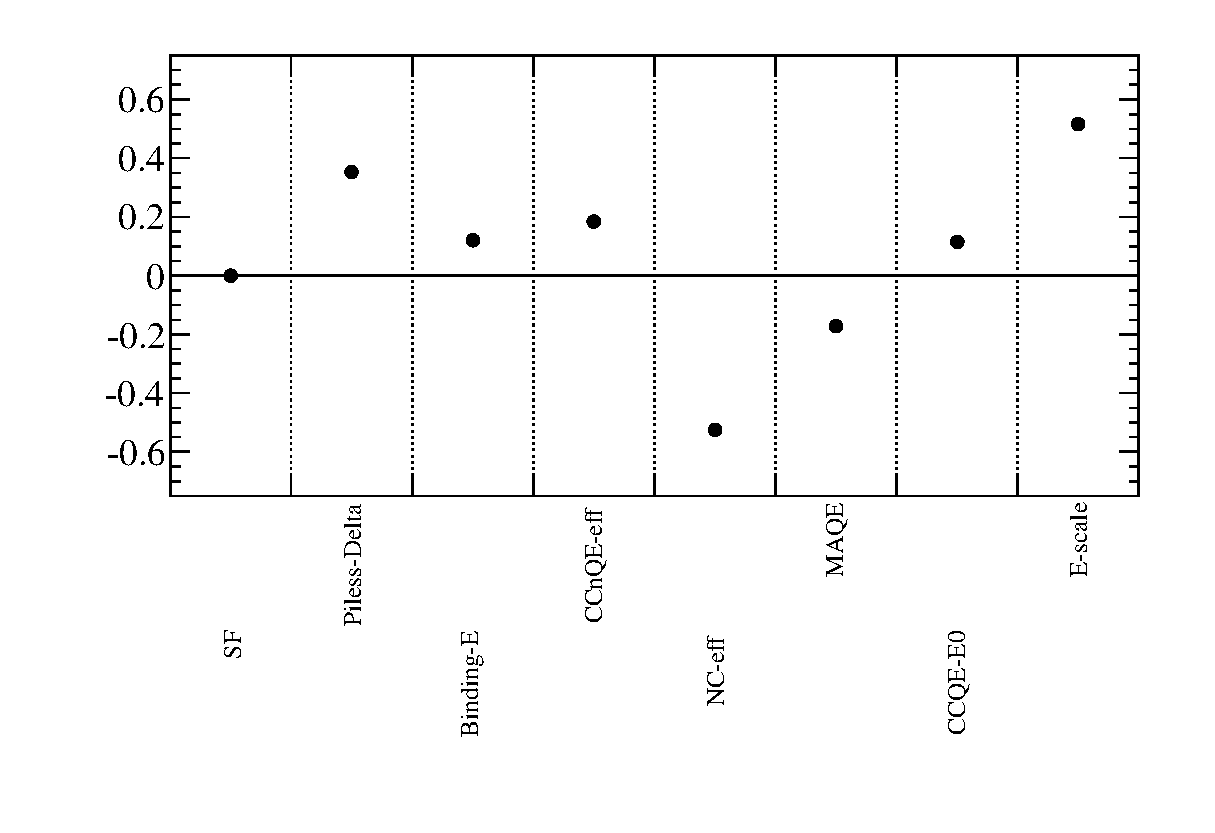
\includegraphics[width=14pc,angle=270]{./images/fit_toymc/example_fits/pulls_0}
\caption {
  Systematic pulls for the 2+8 fit to fake data set 0.
}
\label{fig:fakedata_pulls_0}
\end{minipage}
\hspace{0.06\linewidth}
\begin{minipage}[t]{0.48\linewidth}
\center
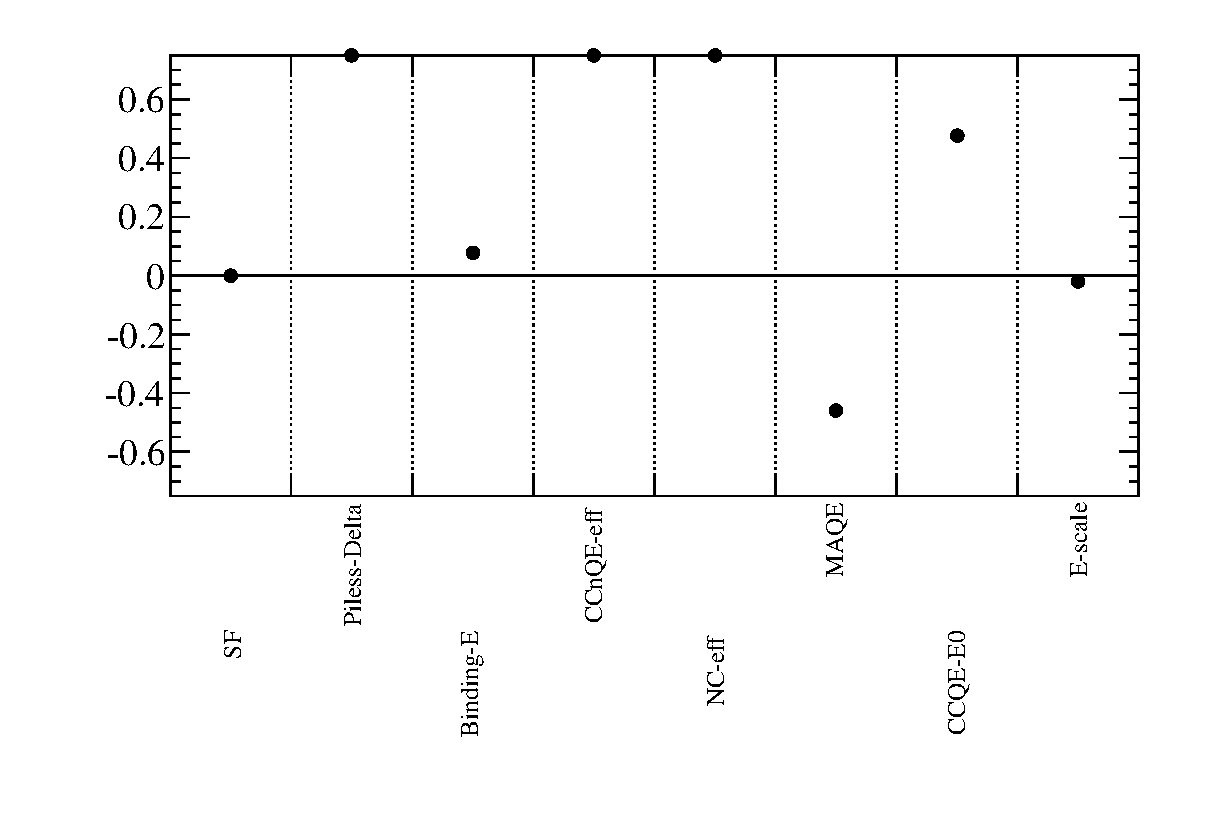
\includegraphics[width=14pc,angle=270]{./images/fit_toymc/example_fits/pulls_1}
\caption { 
  Systematic pulls for the 2+8 fit to fake data set 1.
}
\label{fig:fakedata_pulls_1}
\end{minipage}
\vfill
\begin{minipage}[t]{0.48\linewidth}
\center
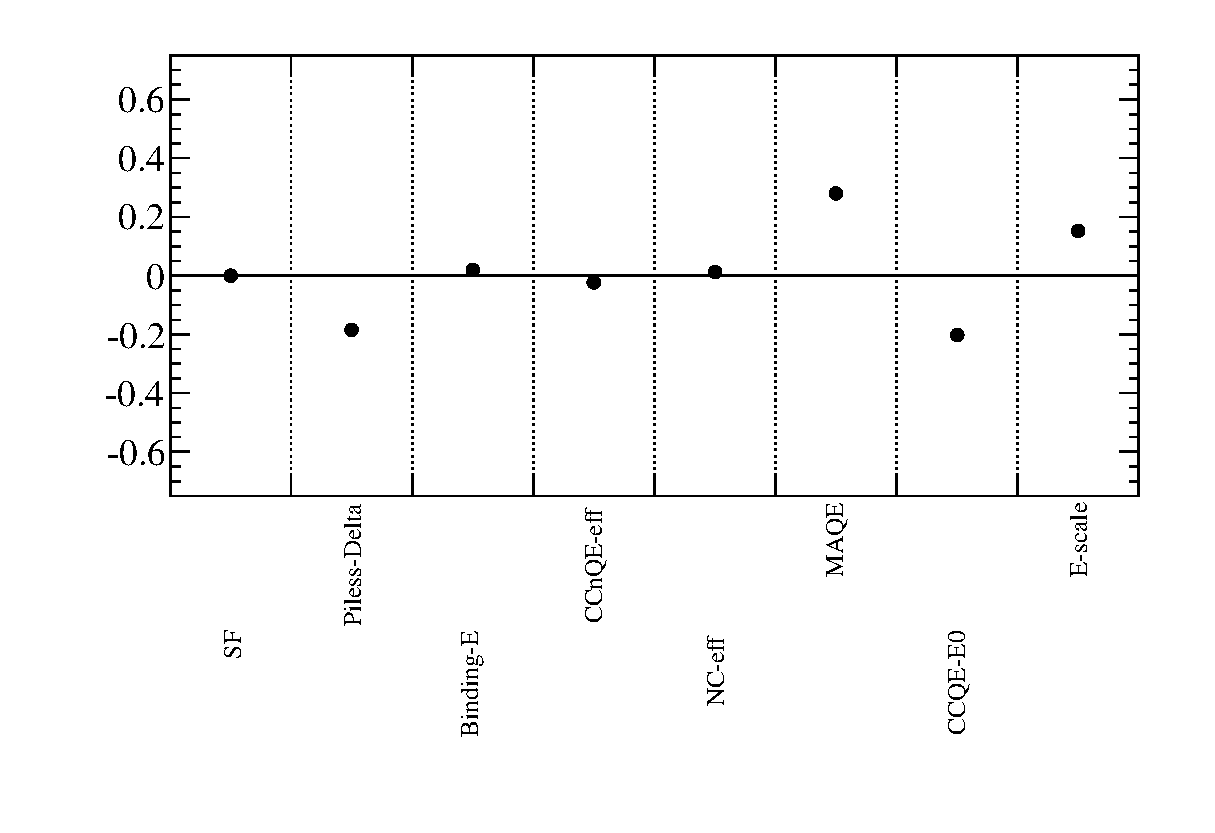
\includegraphics[width=14pc,angle=270]{./images/fit_toymc/example_fits/pulls_2}
\caption {
  Systematic pulls for the 2+8 fit to fake data set 2.
}
\label{fig:fakedata_pulls_2}
\end{minipage}
\hspace{0.06\linewidth}
\begin{minipage}[t]{0.48\linewidth}
\center
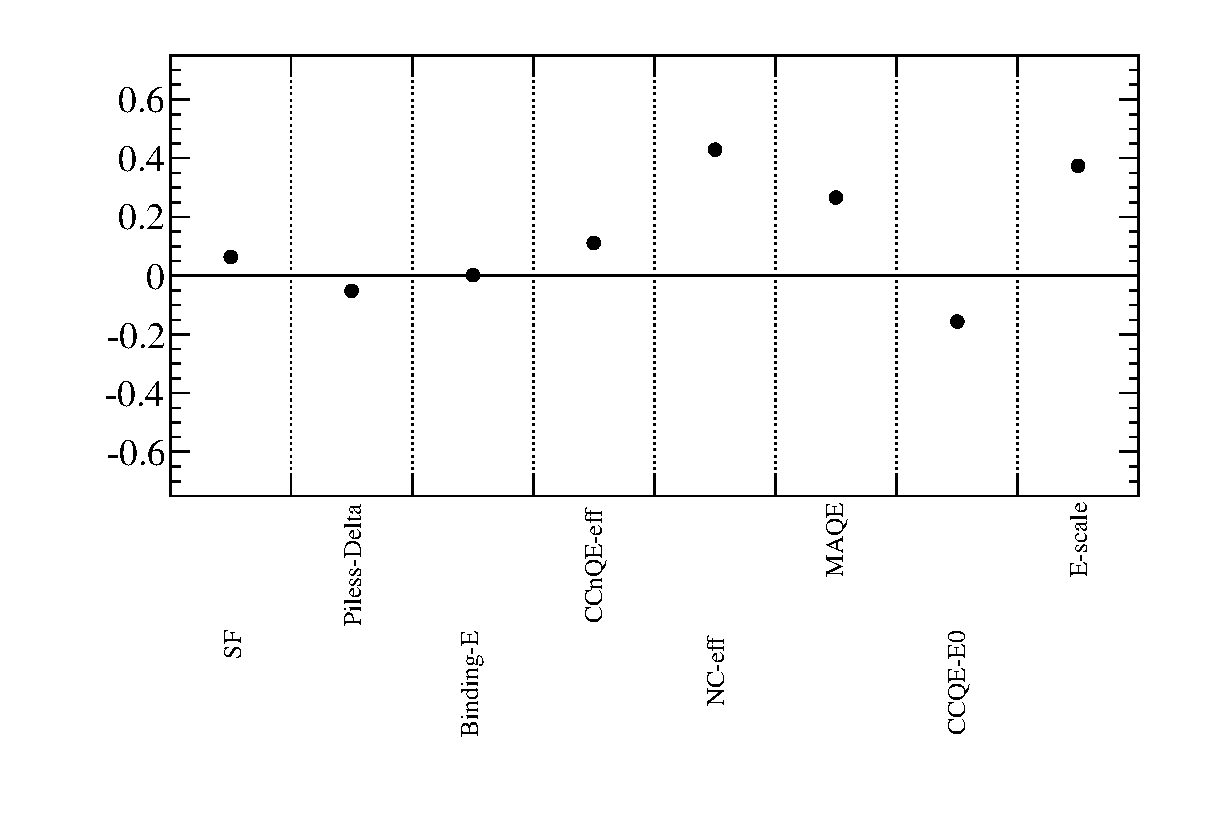
\includegraphics[width=14pc,angle=270]{./images/fit_toymc/example_fits/pulls_3}
\caption { 
  Systematic pulls for the 2+8 fit to fake data set 3.
}
\label{fig:fakedata_pulls_3}
\end{minipage}
\vfill
\begin{minipage}[t]{0.48\linewidth}
\center
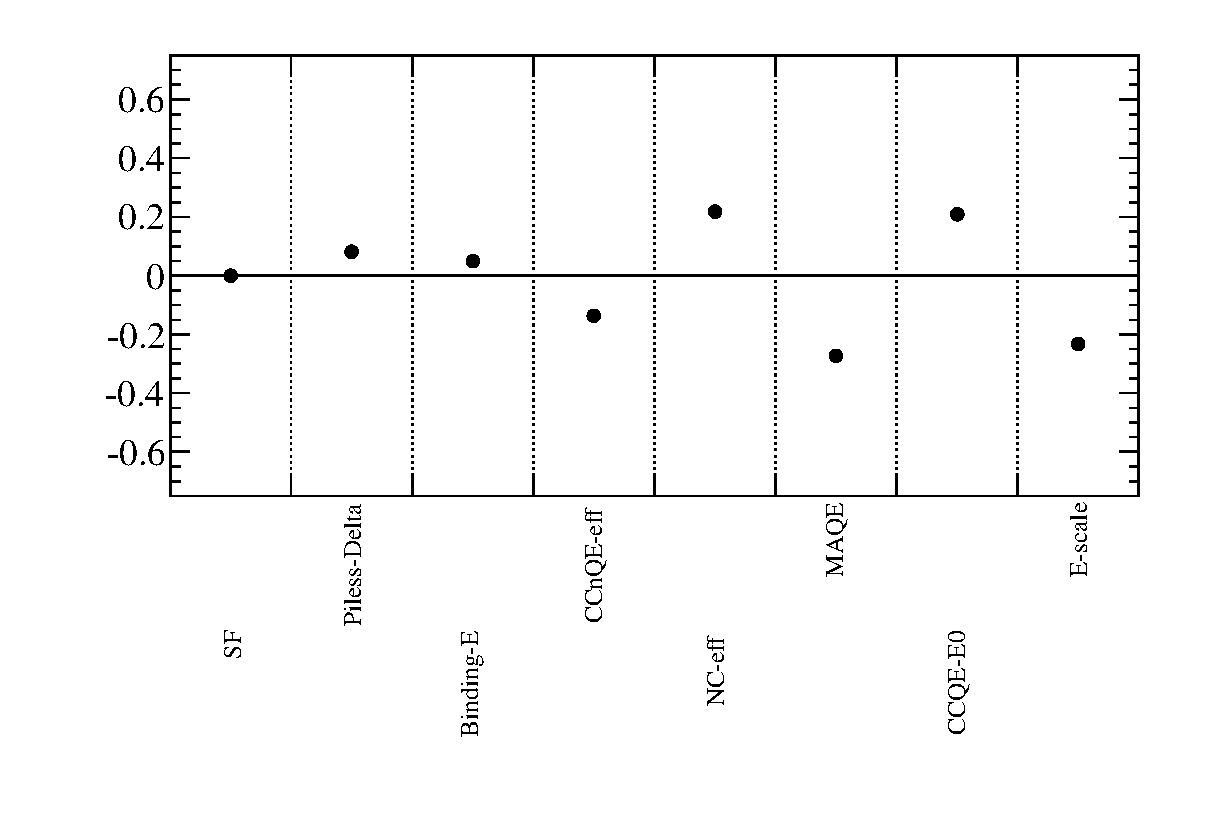
\includegraphics[width=14pc,angle=270]{./images/fit_toymc/example_fits/pulls_4}
\caption {
  Systematic pulls for the 2+8 fit to fake data set 4.
}
\label{fig:fakedata_pulls_4}
\end{minipage}
\hspace{0.06\linewidth}
\begin{minipage}[t]{0.48\linewidth}
\center
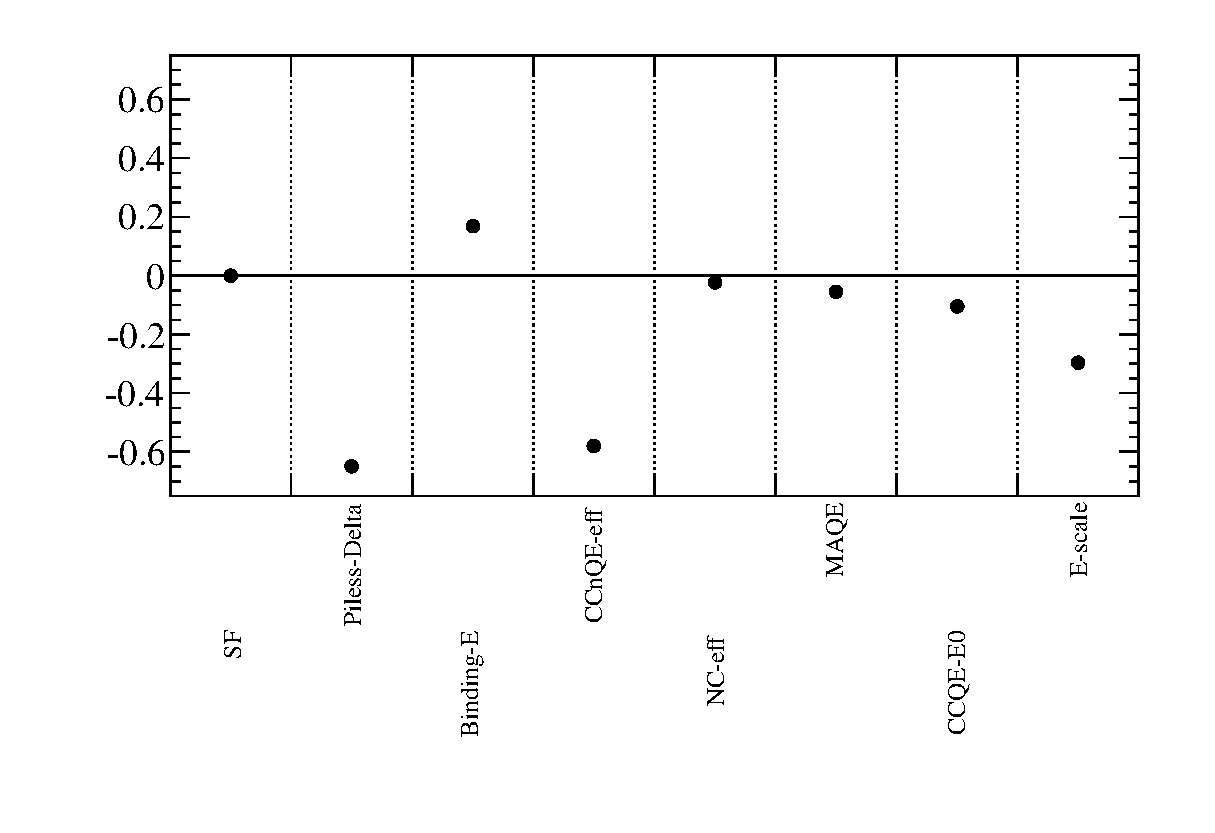
\includegraphics[width=14pc,angle=270]{./images/fit_toymc/example_fits/pulls_5}
\caption { 
  Systematic pulls for the 2+8 fit to fake data set 5.
}
\label{fig:fakedata_pulls_5}
\end{minipage}
\end{figure*}


%...........................................................
%
% Systematic parameter pulls for `2+N' fits
%

\begin{figure*}[htb]
\begin{minipage}[t]{0.48\linewidth}
\center
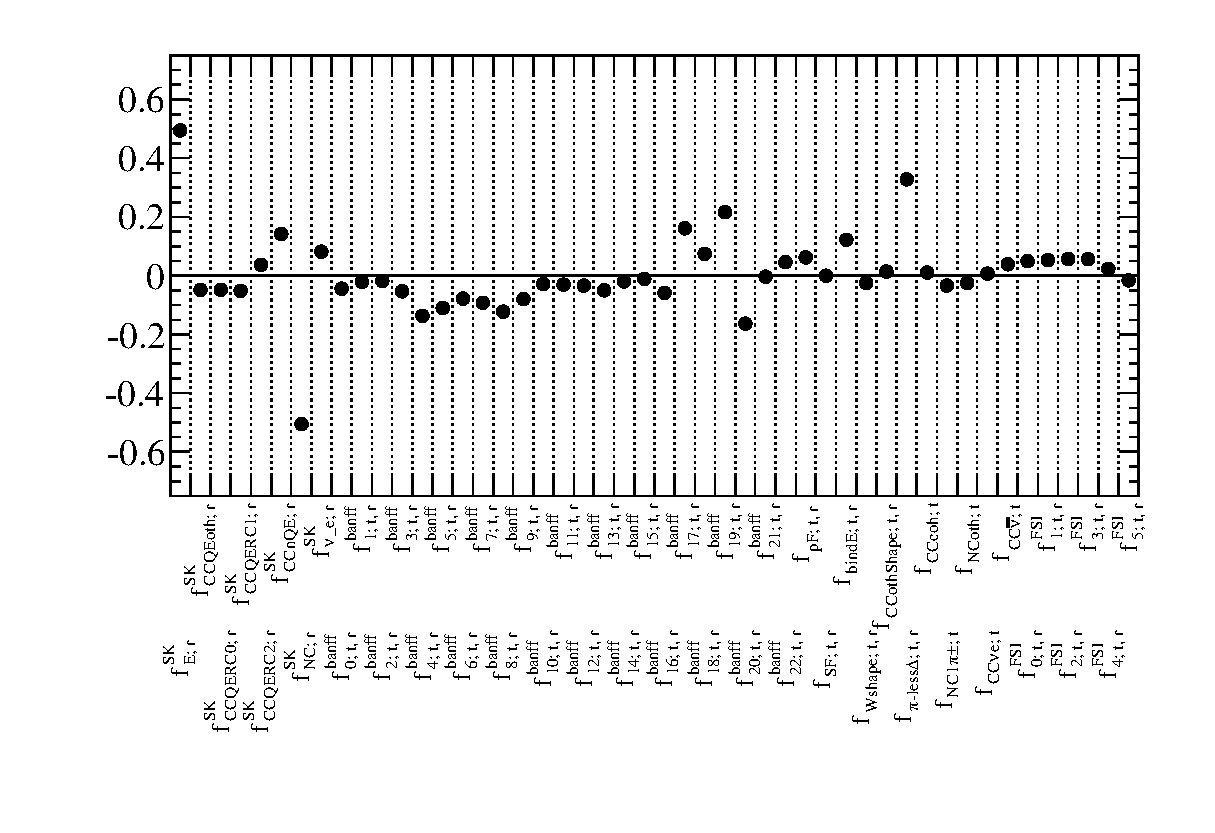
\includegraphics[width=18pc,angle=270]{./images/fit_toymc/example_fits/2N/pulls_0}
\caption {
  Systematic pulls for the 2+N fit to fake data set 0.
}
\label{fig:fakedata_pulls_2N_0}
\end{minipage}
\hspace{0.06\linewidth}
\begin{minipage}[t]{0.48\linewidth}
\center
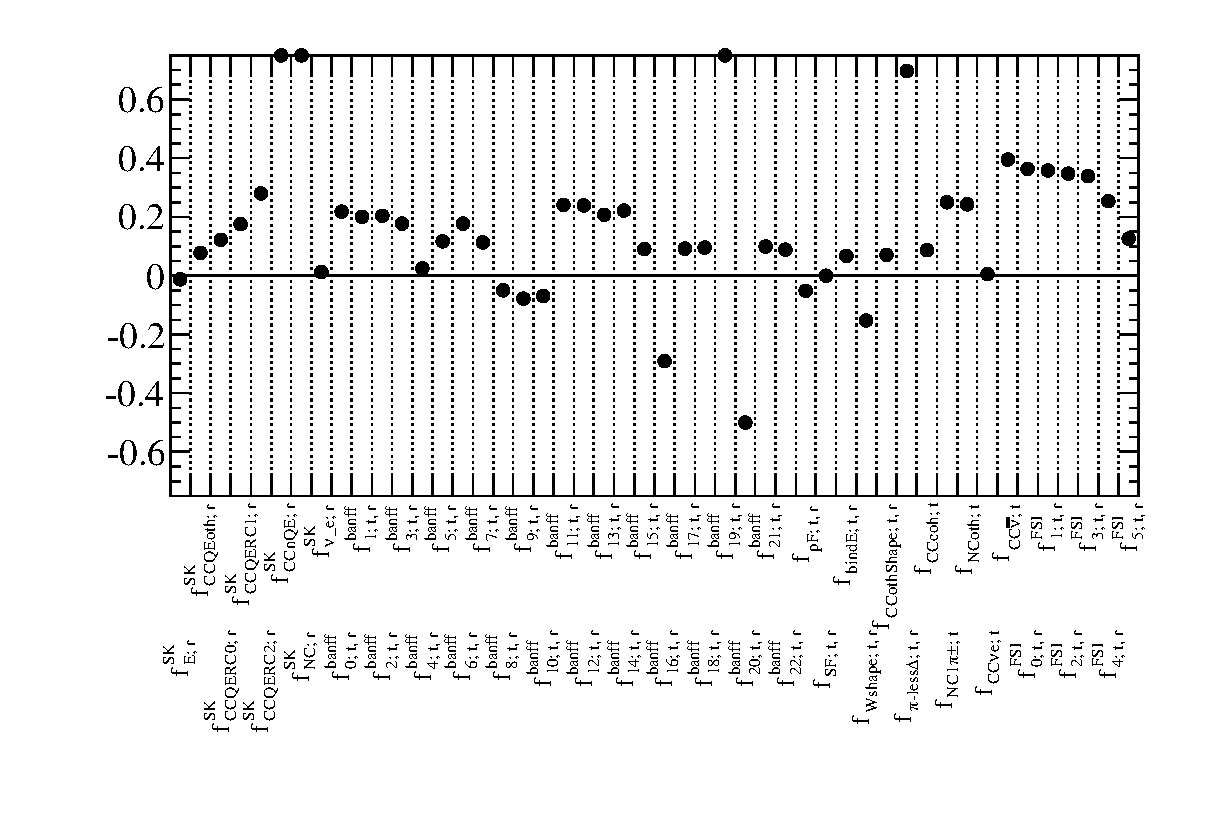
\includegraphics[width=18pc,angle=270]{./images/fit_toymc/example_fits/2N/pulls_1}
\caption { 
  Systematic pulls for the 2+N fit to fake data set 1.
}
\label{fig:fakedata_pulls_2N_1}
\end{minipage}
\vfill
\begin{minipage}[t]{0.48\linewidth}
\center
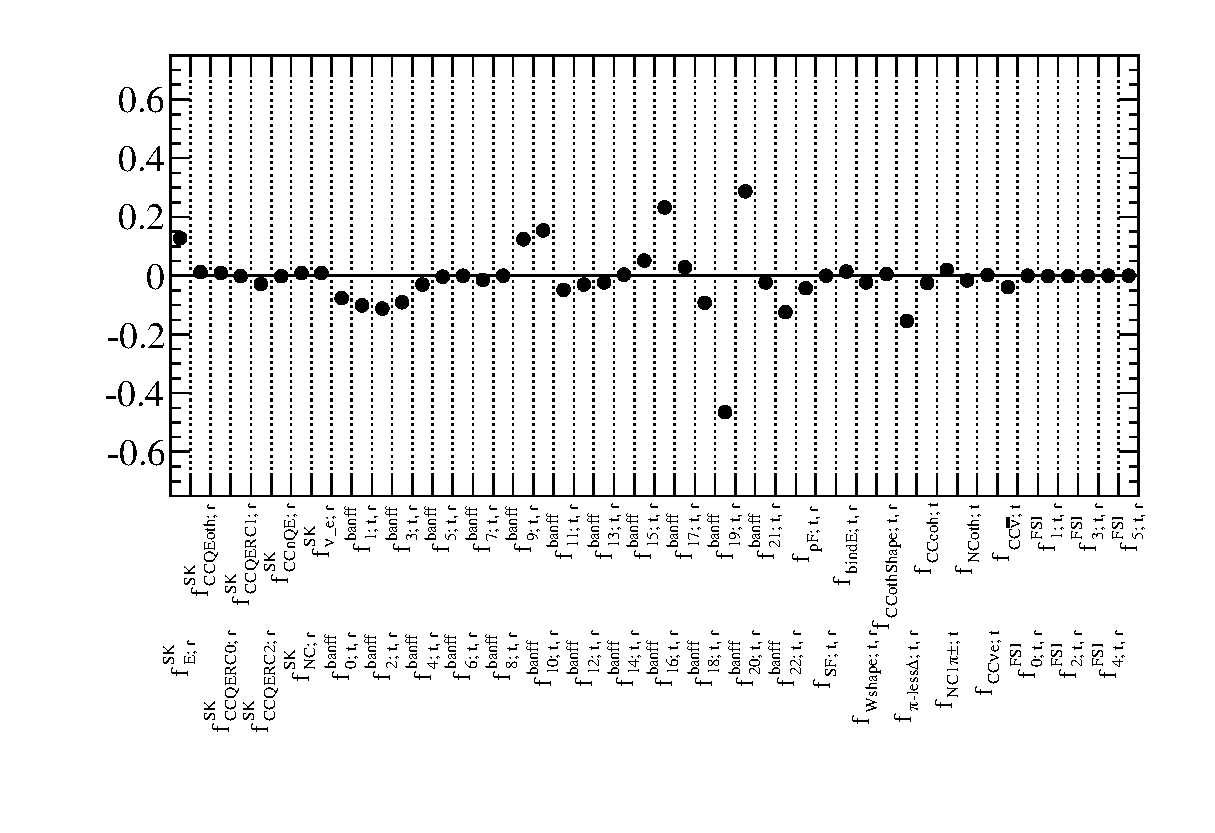
\includegraphics[width=18pc,angle=270]{./images/fit_toymc/example_fits/2N/pulls_2}
\caption {
  Systematic pulls for the 2+N fit to fake data set 2.
}
\label{fig:fakedata_pulls_2N_2}
\end{minipage}
\hspace{0.06\linewidth}
\begin{minipage}[t]{0.48\linewidth}
\center
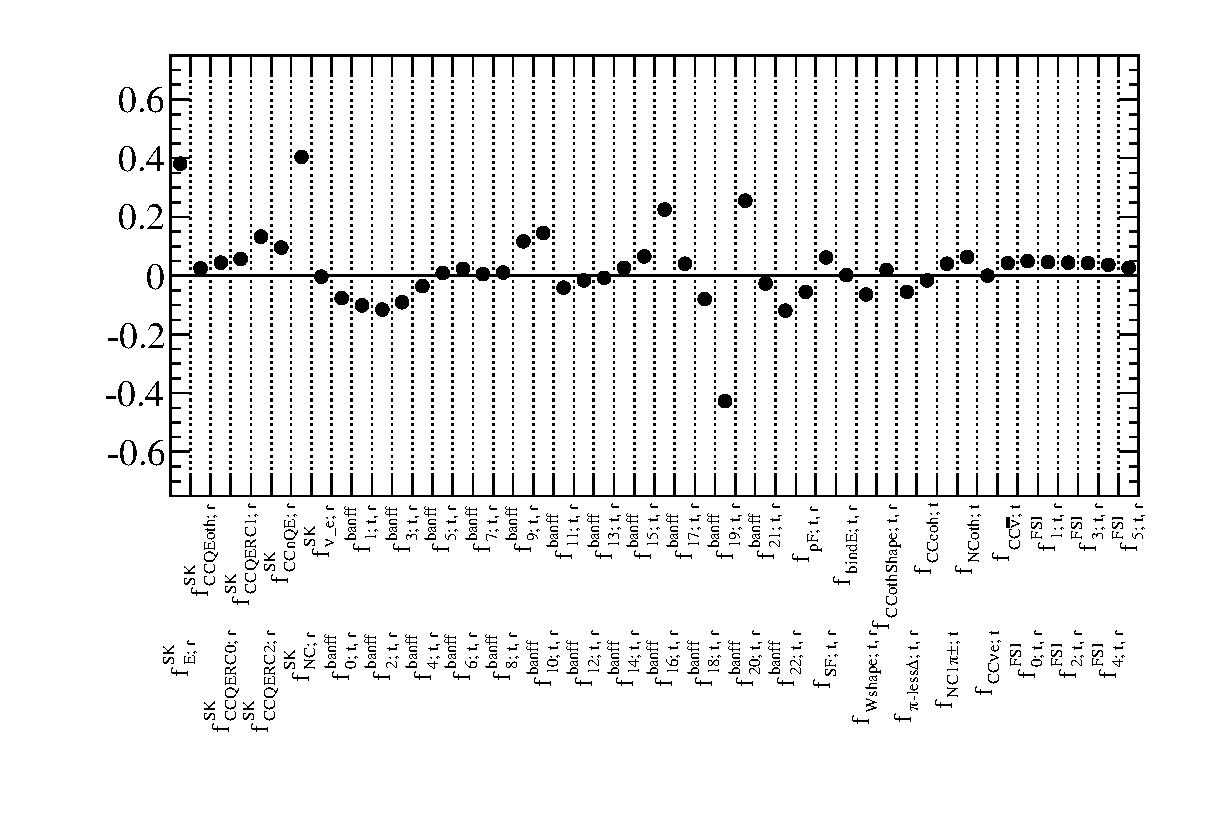
\includegraphics[width=18pc,angle=270]{./images/fit_toymc/example_fits/2N/pulls_3}
\caption { 
  Systematic pulls for the 2+N fit to fake data set 3.
}
\label{fig:fakedata_pulls_2N_3}
\end{minipage}
\vfill
\begin{minipage}[t]{0.48\linewidth}
\center
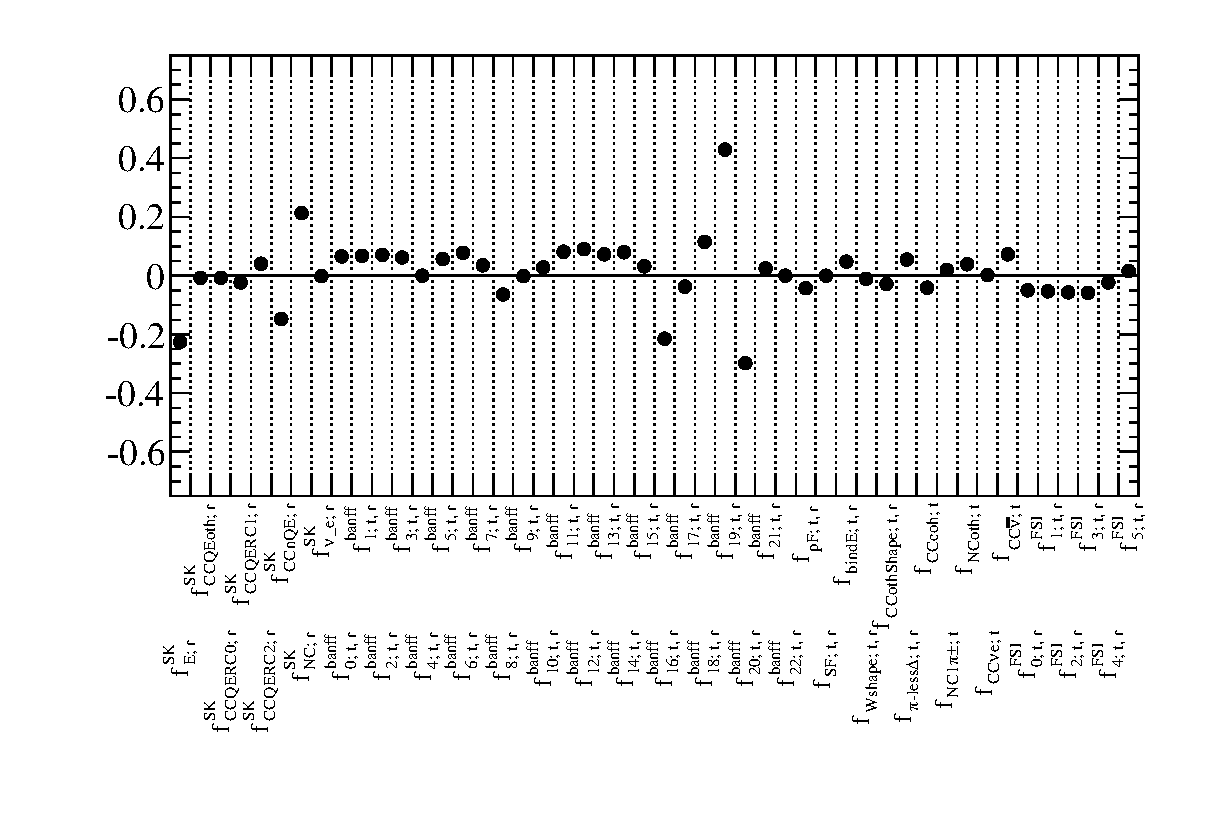
\includegraphics[width=18pc,angle=270]{./images/fit_toymc/example_fits/2N/pulls_4}
\caption {
  Systematic pulls for the 2+N fit to fake data set 4.
}
\label{fig:fakedata_pulls_2N_4}
\end{minipage}
\hspace{0.06\linewidth}
\begin{minipage}[t]{0.48\linewidth}
\center
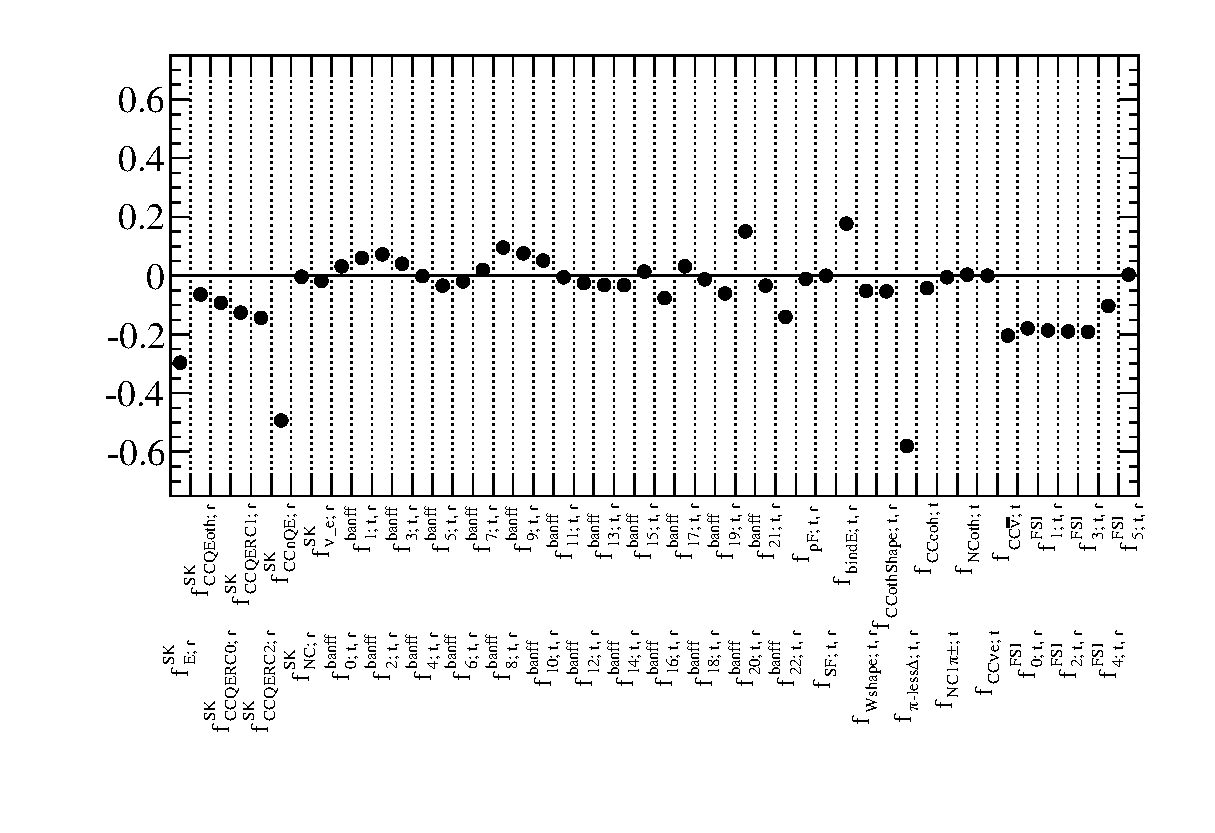
\includegraphics[width=18pc,angle=270]{./images/fit_toymc/example_fits/2N/pulls_5}
\caption { 
  Systematic pulls for the 2+N fit to fake data set 5.
}
\label{fig:fakedata_pulls_2N_5}
\end{minipage}
\end{figure*}

\clearpage

\subsection{Goodness of fit}
\label{appendix:example_toy_mc_fits:goodness}

%...........................................................
%
% Goodness of fit for `2+N' fits
%

% \begin{figure*}[htb]
% \begin{minipage}[t]{0.48\linewidth}
% \center
% \includegraphics[width=18pc]{./images/fit_toymc/example_fits/2N/goodness_0}
% \caption {
%   Distribution of $\chi^2_{gof}$ from 1000 toy MC at the best fit oscillation point for the 2+N fit to fake data set 0.
%   The $\chi^2_{gof}$ for data is highlighted.
% }
% \label{fig:fakedata_goodness_2N_0}
% \end{minipage}
% \hspace{0.06\linewidth}
% \begin{minipage}[t]{0.48\linewidth}
% \center
% \includegraphics[width=18pc]{./images/fit_toymc/example_fits/2N/goodness_1}
% \caption { 
%   Distribution of $\chi^2_{gof}$ from 1000 toy MC at the best fit oscillation point for the 2+N fit to fake data set 1.
%   The $\chi^2_{gof}$ for data is highlighted.
% }
% \label{fig:fakedata_goodness_2N_1}
% \end{minipage}
% \vfill
% \begin{minipage}[t]{0.48\linewidth}
% \center
% \includegraphics[width=18pc]{./images/fit_toymc/example_fits/2N/goodness_2}
% \caption {
%   Distribution of $\chi^2_{gof}$ from 1000 toy MC at the best fit oscillation point for the 2+N fit to fake data set 2.
%   The $\chi^2_{gof}$ for data is highlighted.
% }
% \label{fig:fakedata_goodness_2N_2}
% \end{minipage}
% \hspace{0.06\linewidth}
% \begin{minipage}[t]{0.48\linewidth}
% \center
% \includegraphics[width=18pc]{./images/fit_toymc/example_fits/2N/goodness_3}
% \caption { 
%   Distribution of $\chi^2_{gof}$ from 1000 toy MC at the best fit oscillation point for the 2+N fit to fake data set 3.
%   The $\chi^2_{gof}$ for data is highlighted.
% }
% \label{fig:fakedata_goodness_2N_3}
% \end{minipage}
% \vfill
% \begin{minipage}[t]{0.48\linewidth}
% \center
% \includegraphics[width=18pc]{./images/fit_toymc/example_fits/2N/goodness_4}
% \caption {
%   Distribution of $\chi^2_{gof}$ from 1000 toy MC at the best fit oscillation point for the 2+N fit to fake data set 4.
%   The $\chi^2_{gof}$ for data is highlighted.
% }
% \label{fig:fakedata_goodness_2N_4}
% \end{minipage}
% \hspace{0.06\linewidth}
% \begin{minipage}[t]{0.48\linewidth}
% \center
% \includegraphics[width=18pc]{./images/fit_toymc/example_fits/2N/goodness_5}
% \caption { 
%   Distribution of $\chi^2_{gof}$ from 1000 toy MC at the best fit oscillation point for the 2+N fit to fake data set 5.
%   The $\chi^2_{gof}$ for data is highlighted.
% }
% \label{fig:fakedata_goodness_2N_5}
% \end{minipage}
% \end{figure*}

%...........................................................
%
% Goodness of fit for `2+8' fits
%

\begin{figure*}[htb]
\begin{minipage}[t]{0.48\linewidth}
\center
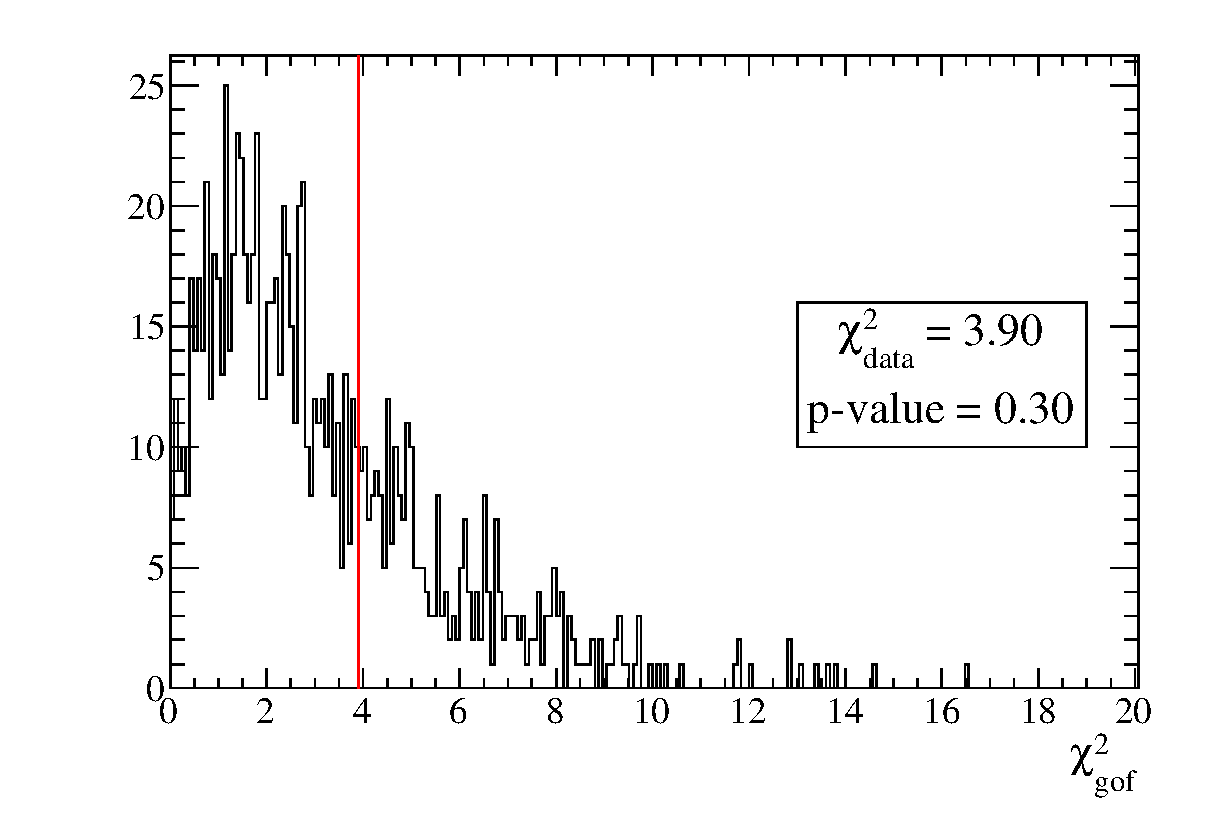
\includegraphics[width=18pc]{./images/fit_toymc/example_fits/goodness_0}
\caption {
  Distribution of $\chi^2_{gof}$ from 1000 toy MC datasets at the best-fit oscillation point for the 2+8 fit to fake data set 0.
  The $\chi^2_{gof}$ for data is highlighted.
}
\label{fig:fakedata_goodness_0}
\end{minipage}
\hspace{0.06\linewidth}
\begin{minipage}[t]{0.48\linewidth}
\center
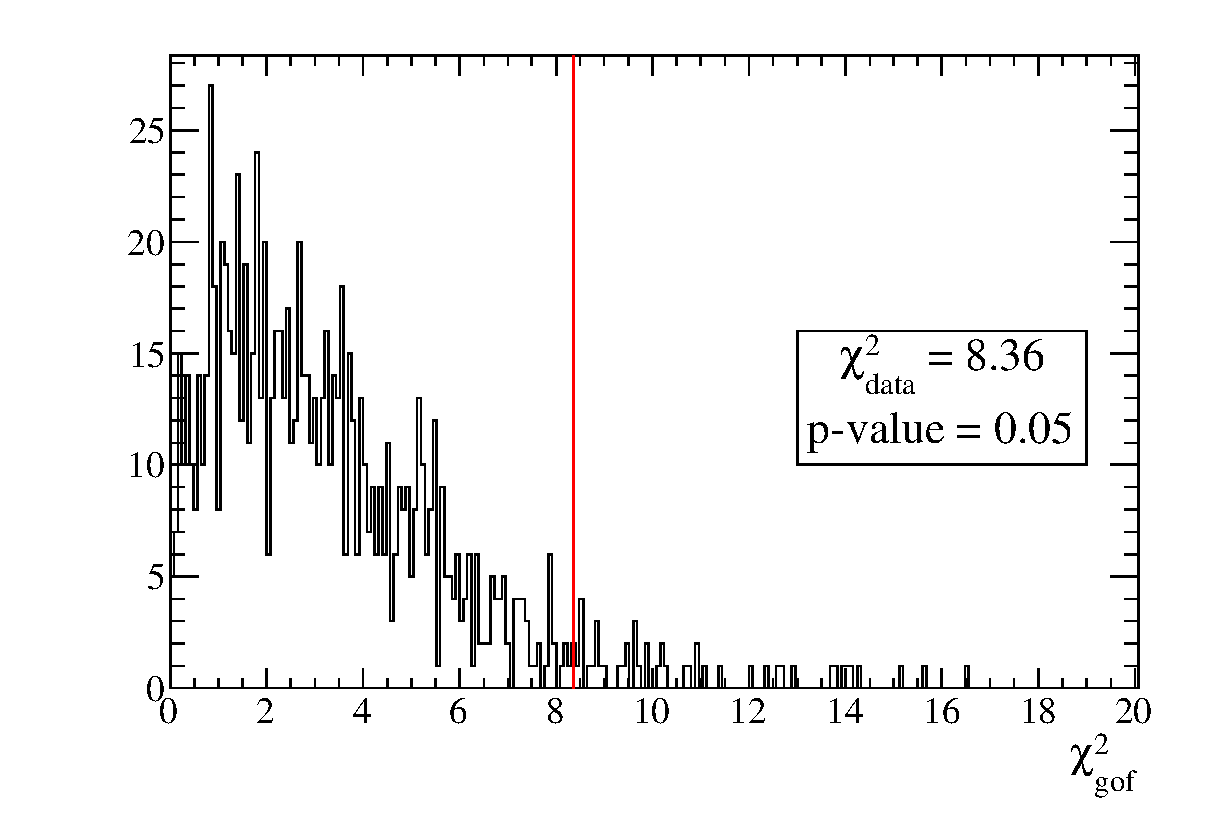
\includegraphics[width=18pc]{./images/fit_toymc/example_fits/goodness_1}
\caption { 
  Distribution of $\chi^2_{gof}$ from 1000 toy MC datasets at the best-fit oscillation point for the 2+8 fit to fake data set 1.
  The $\chi^2_{gof}$ for data is highlighted.
}
\label{fig:fakedata_goodness_1}
\end{minipage}
\vfill
\begin{minipage}[t]{0.48\linewidth}
\center
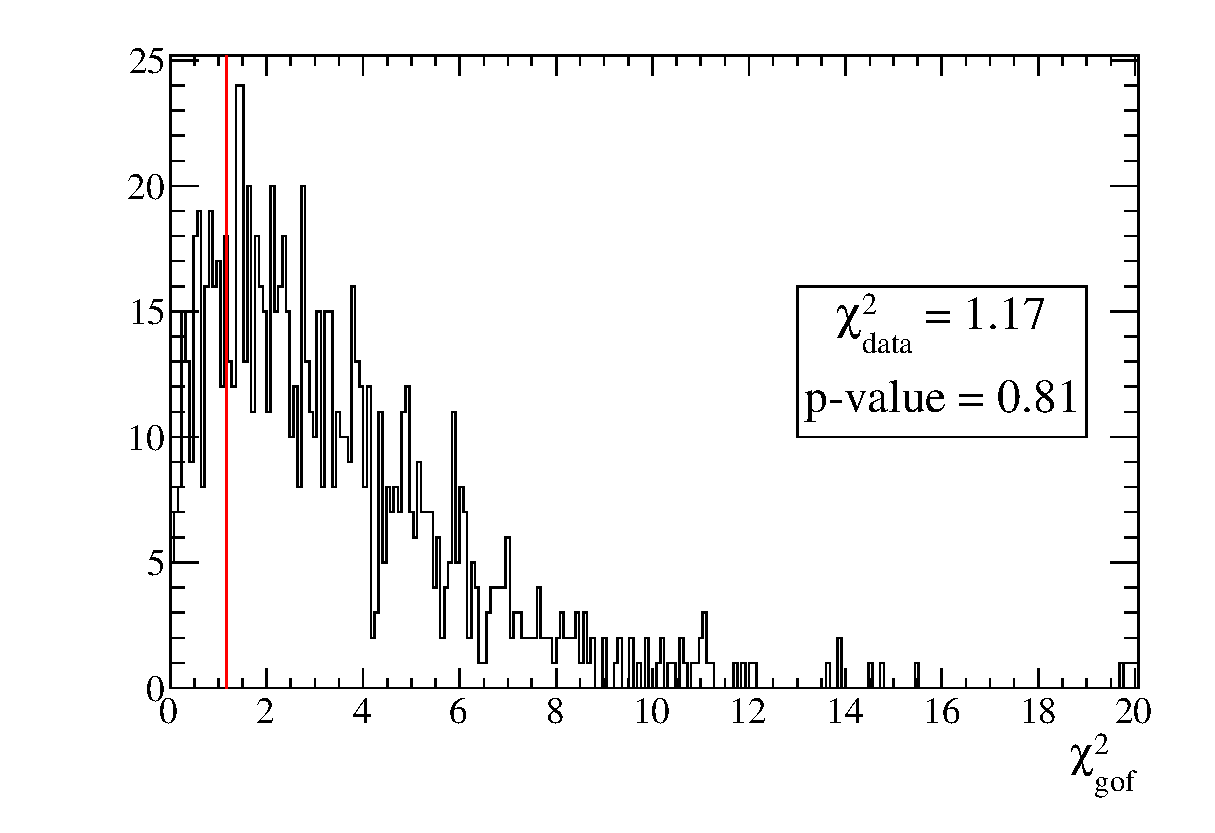
\includegraphics[width=18pc]{./images/fit_toymc/example_fits/goodness_2}
\caption {
  Distribution of $\chi^2_{gof}$ from 1000 toy MC datasets at the best-fit oscillation point for the 2+8 fit to fake data set 2.
  The $\chi^2_{gof}$ for data is highlighted.
}
\label{fig:fakedata_goodness_2}
\end{minipage}
\hspace{0.06\linewidth}
\begin{minipage}[t]{0.48\linewidth}
\center
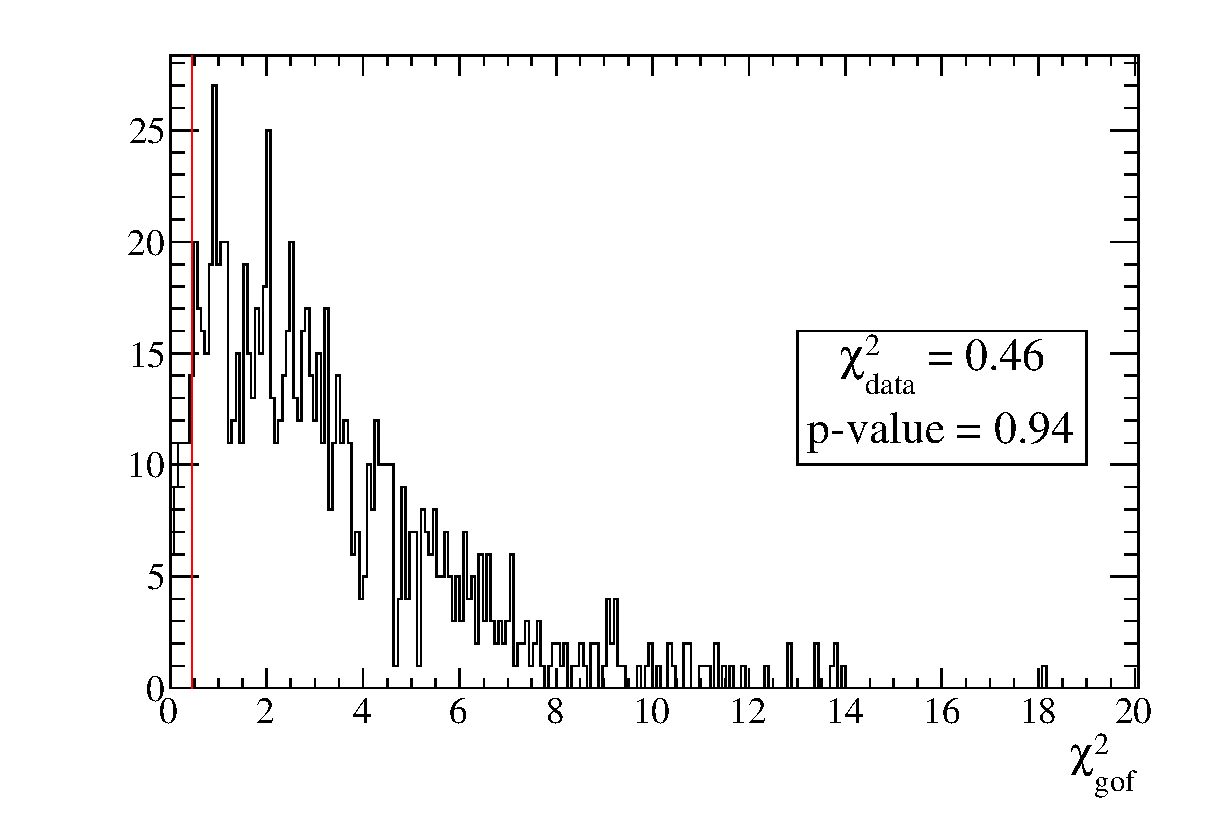
\includegraphics[width=18pc]{./images/fit_toymc/example_fits/goodness_3}
\caption { 
  Distribution of $\chi^2_{gof}$ from 1000 toy MC datasets at the best-fit oscillation point for the 2+8 fit to fake data set 3.
  The $\chi^2_{gof}$ for data is highlighted.
}
\label{fig:fakedata_goodness_3}
\end{minipage}
\vfill
\begin{minipage}[t]{0.48\linewidth}
\center
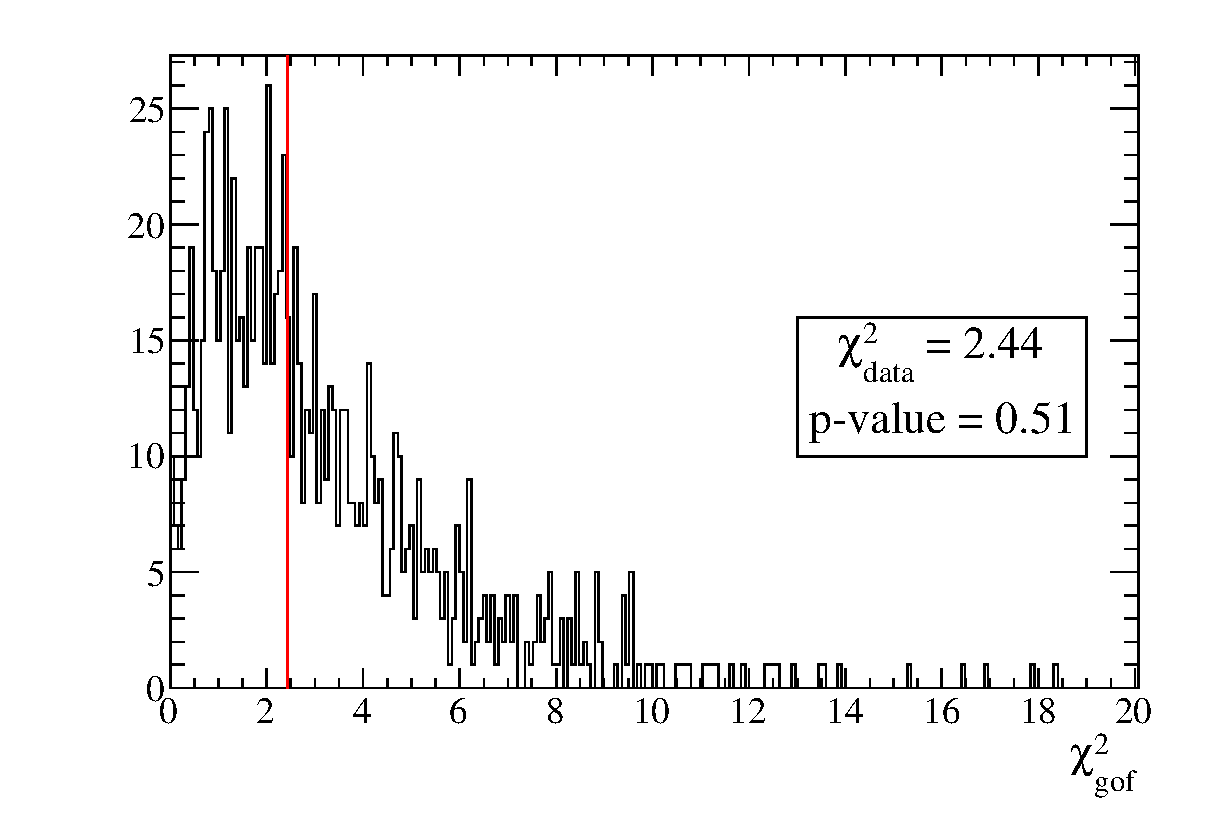
\includegraphics[width=18pc]{./images/fit_toymc/example_fits/goodness_4}
\caption {
  Distribution of $\chi^2_{gof}$ from 1000 toy MC datasets at the best-fit oscillation point for the 2+8 fit to fake data set 4.
  The $\chi^2_{gof}$ for data is highlighted.
}
\label{fig:fakedata_goodness_4}
\end{minipage}
\hspace{0.06\linewidth}
\begin{minipage}[t]{0.48\linewidth}
\center
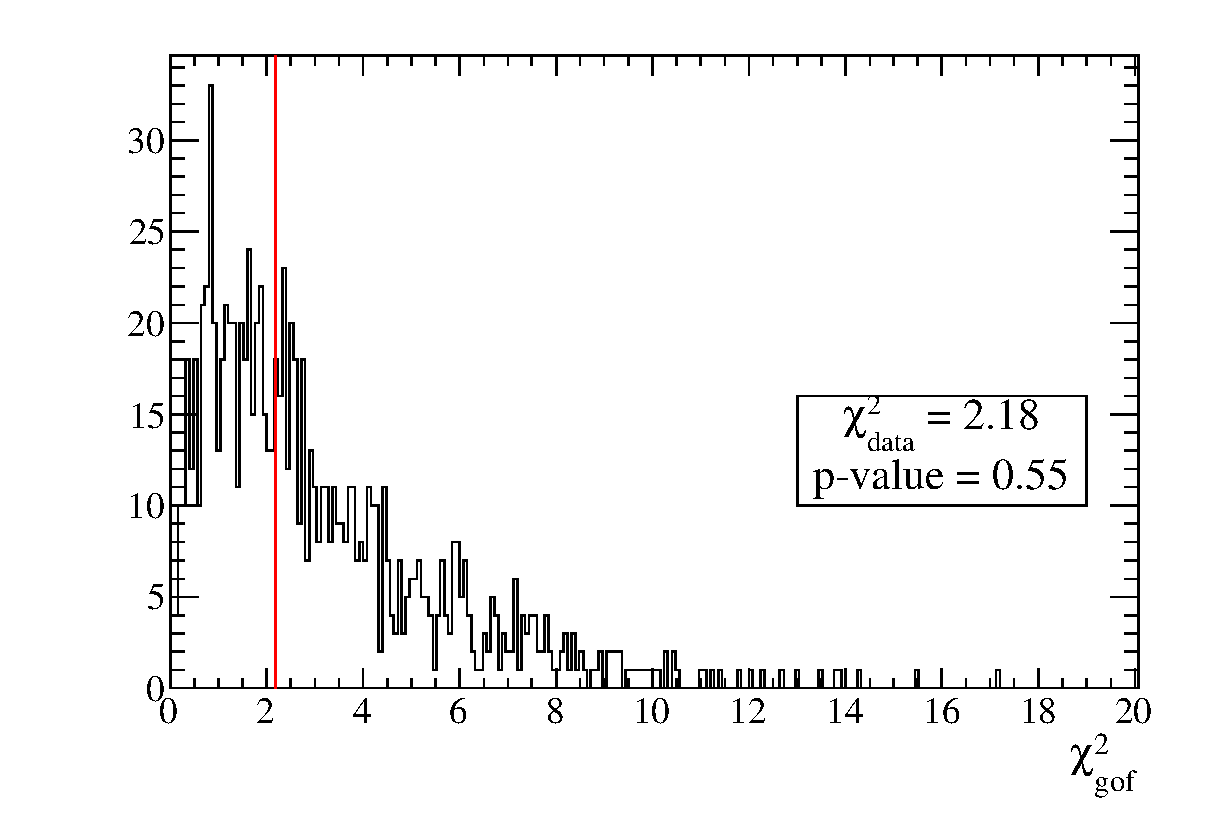
\includegraphics[width=18pc]{./images/fit_toymc/example_fits/goodness_5}
\caption { 
  Distribution of $\chi^2_{gof}$ from 1000 toy MC datasets at the best-fit oscillation point for the 2+8 fit to fake data set 5.
  The $\chi^2_{gof}$ for data is highlighted.
}
\label{fig:fakedata_goodness_5}
\end{minipage}
\end{figure*}


\clearpage
\subsection{Best-fit spectra}
\label{appendix:example_toy_mc_fits:spectra}

%...........................................................
%
% Best-fit spectra and ratios for `2+N' fits
%

\begin{figure*}[htb]
\begin{minipage}[t]{0.48\linewidth}
\center
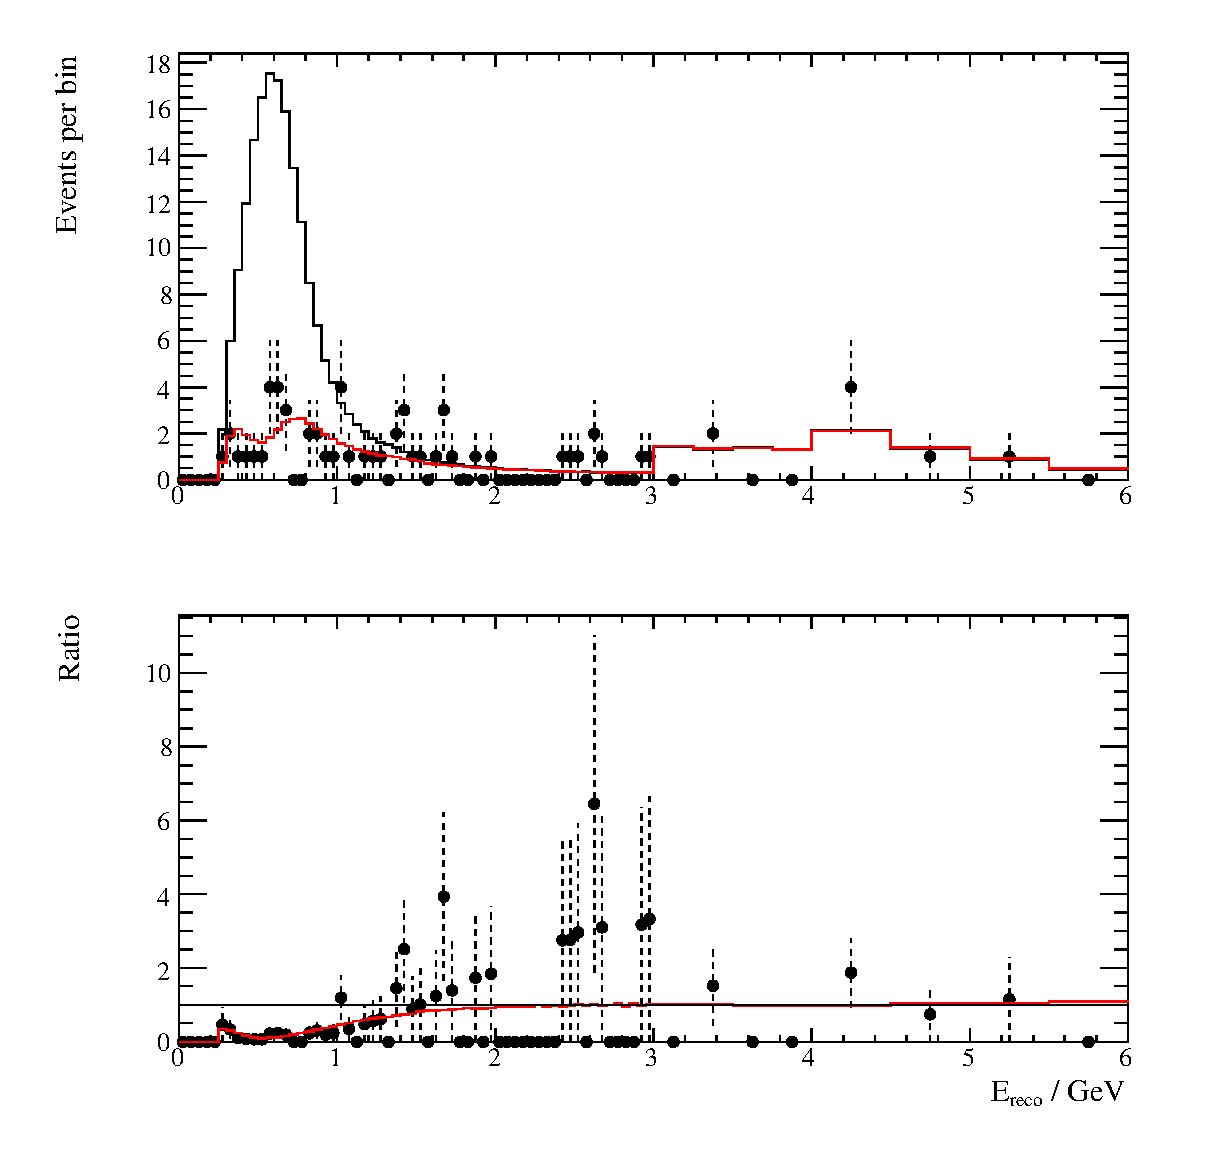
\includegraphics[width=13pc]{./images/fit_toymc/example_fits/2N/spectrum_0}
\caption {
  Best-fit spectrum (top) and ratios of data and best-fit spectrum to predicted spectrum 
  for no oscillations (bottom) for the 2+N fit to fake data set 0
}
\label{fig:fakedata_spectrum_2N_0}
\end{minipage}
\hspace{0.06\linewidth}
\begin{minipage}[t]{0.48\linewidth}
\center
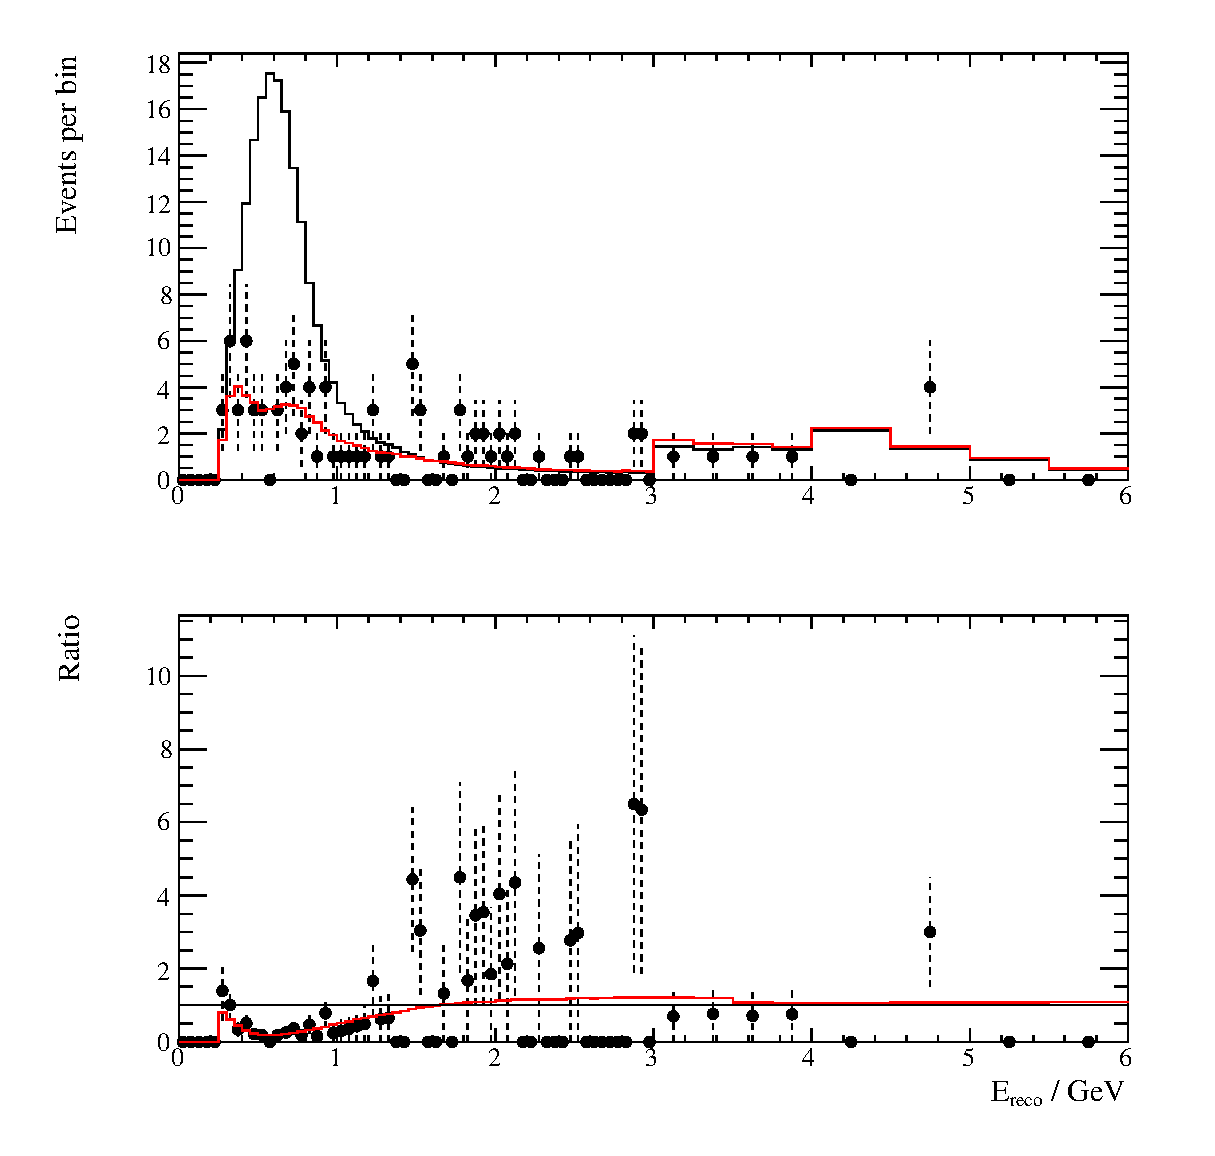
\includegraphics[width=13pc]{./images/fit_toymc/example_fits/2N/spectrum_1}
\caption { 
  Best-fit spectrum (top) and ratios of data and best-fit spectrum to predicted spectrum
  for no oscillations (bottom) for the 2+N fit to fake data set 1
}
\label{fig:fakedata_spectrum_2N_1}
\end{minipage}
\vfill
\begin{minipage}[t]{0.48\linewidth}
\center
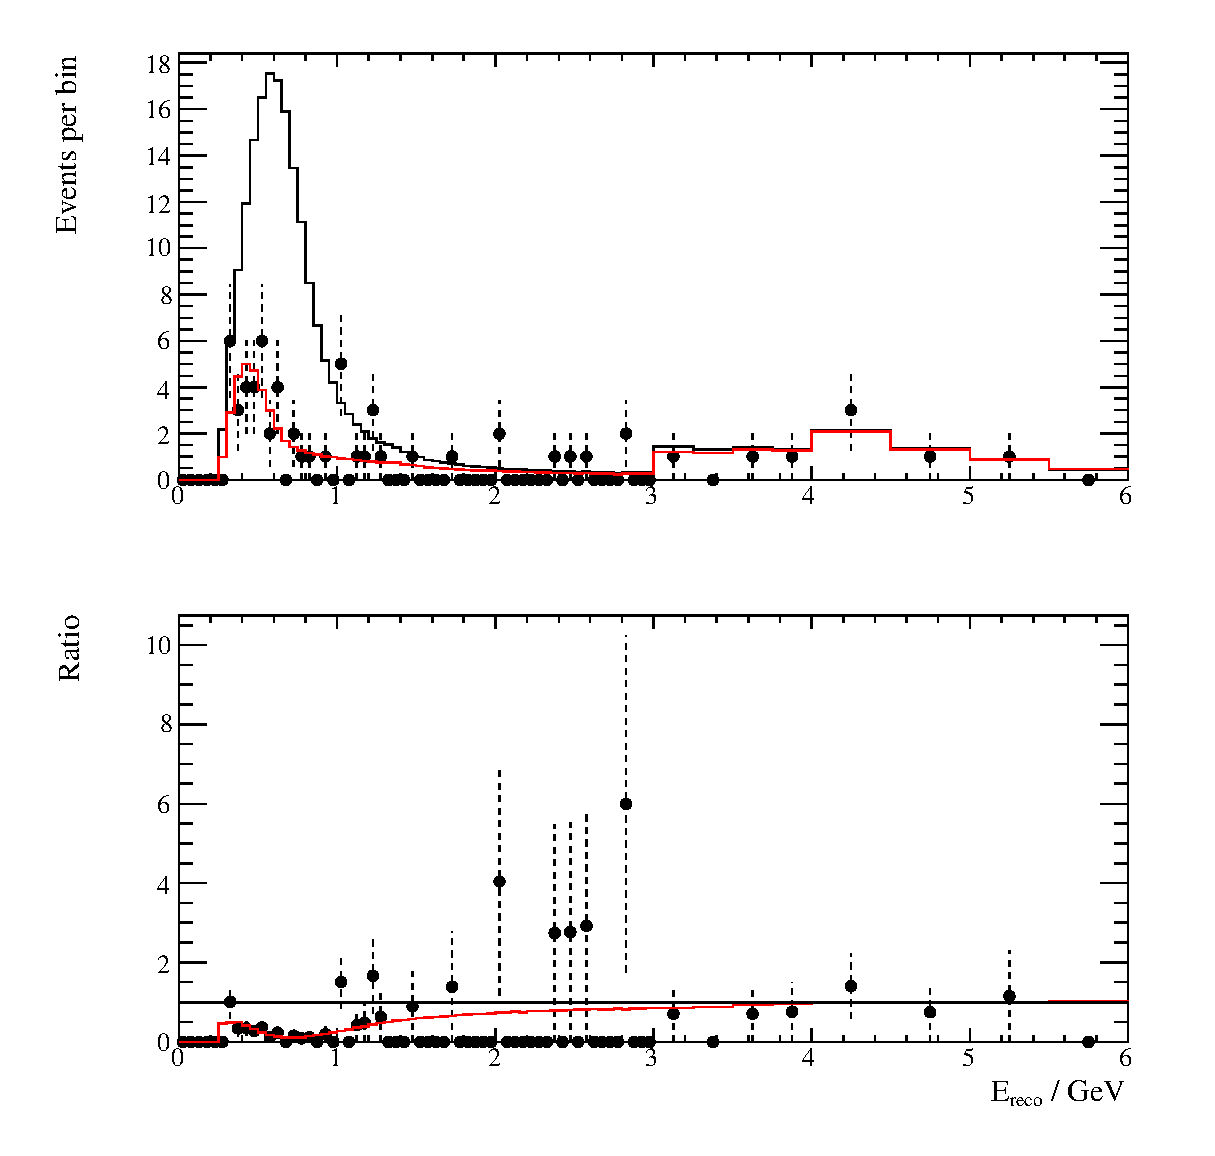
\includegraphics[width=13pc]{./images/fit_toymc/example_fits/2N/spectrum_2}
\caption {
  Best-fit spectrum (top) and ratios of data and best-fit spectrum to predicted spectrum
  for no oscillations (bottom) for the 2+N fit to fake data set 2
}
\label{fig:fakedata_spectrum_2N_2}
\end{minipage}
\hspace{0.06\linewidth}
\begin{minipage}[t]{0.48\linewidth}
\center
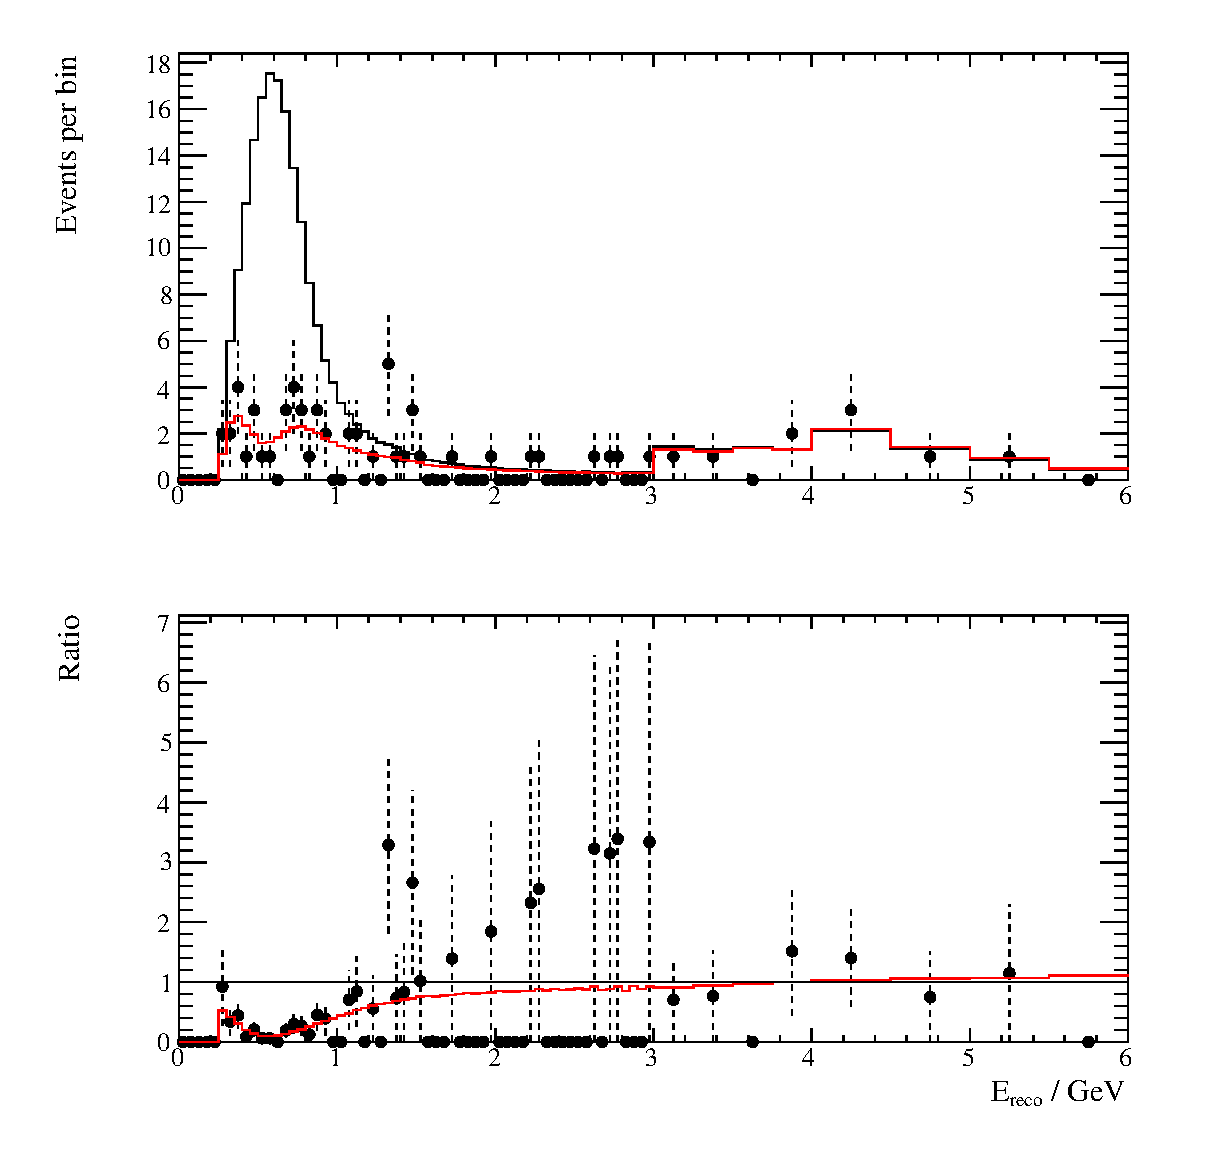
\includegraphics[width=13pc]{./images/fit_toymc/example_fits/2N/spectrum_3}
\caption { 
  Best-fit spectrum (top) and ratios of data and best-fit spectrum to predicted spectrum
  for no oscillations (bottom) for the 2+N fit to fake data set 3
}
\label{fig:fakedata_spectrum_2N_3}
\end{minipage}
\vfill
\begin{minipage}[t]{0.48\linewidth}
\center
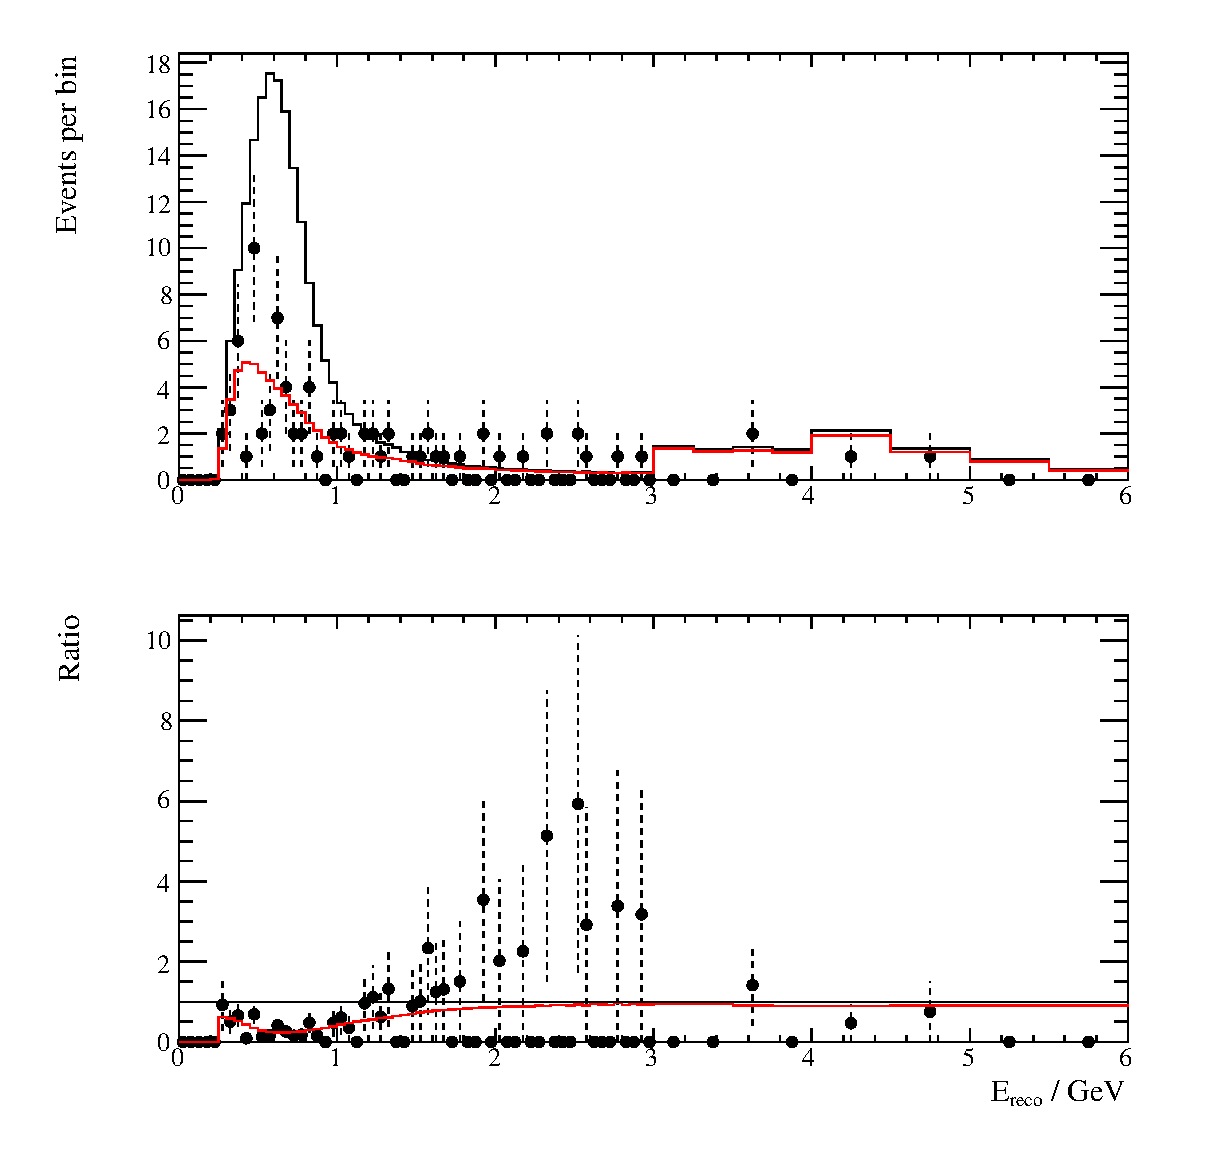
\includegraphics[width=13pc]{./images/fit_toymc/example_fits/2N/spectrum_4}
\caption {
  Best-fit spectrum (top) and ratios of data and best-fit spectrum to predicted spectrum
  for no oscillations (bottom) for the 2+N fit to fake data set 4
}
\label{fig:fakedata_spectrum_2N_4}
\end{minipage}
\hspace{0.06\linewidth}
\begin{minipage}[t]{0.48\linewidth}
\center
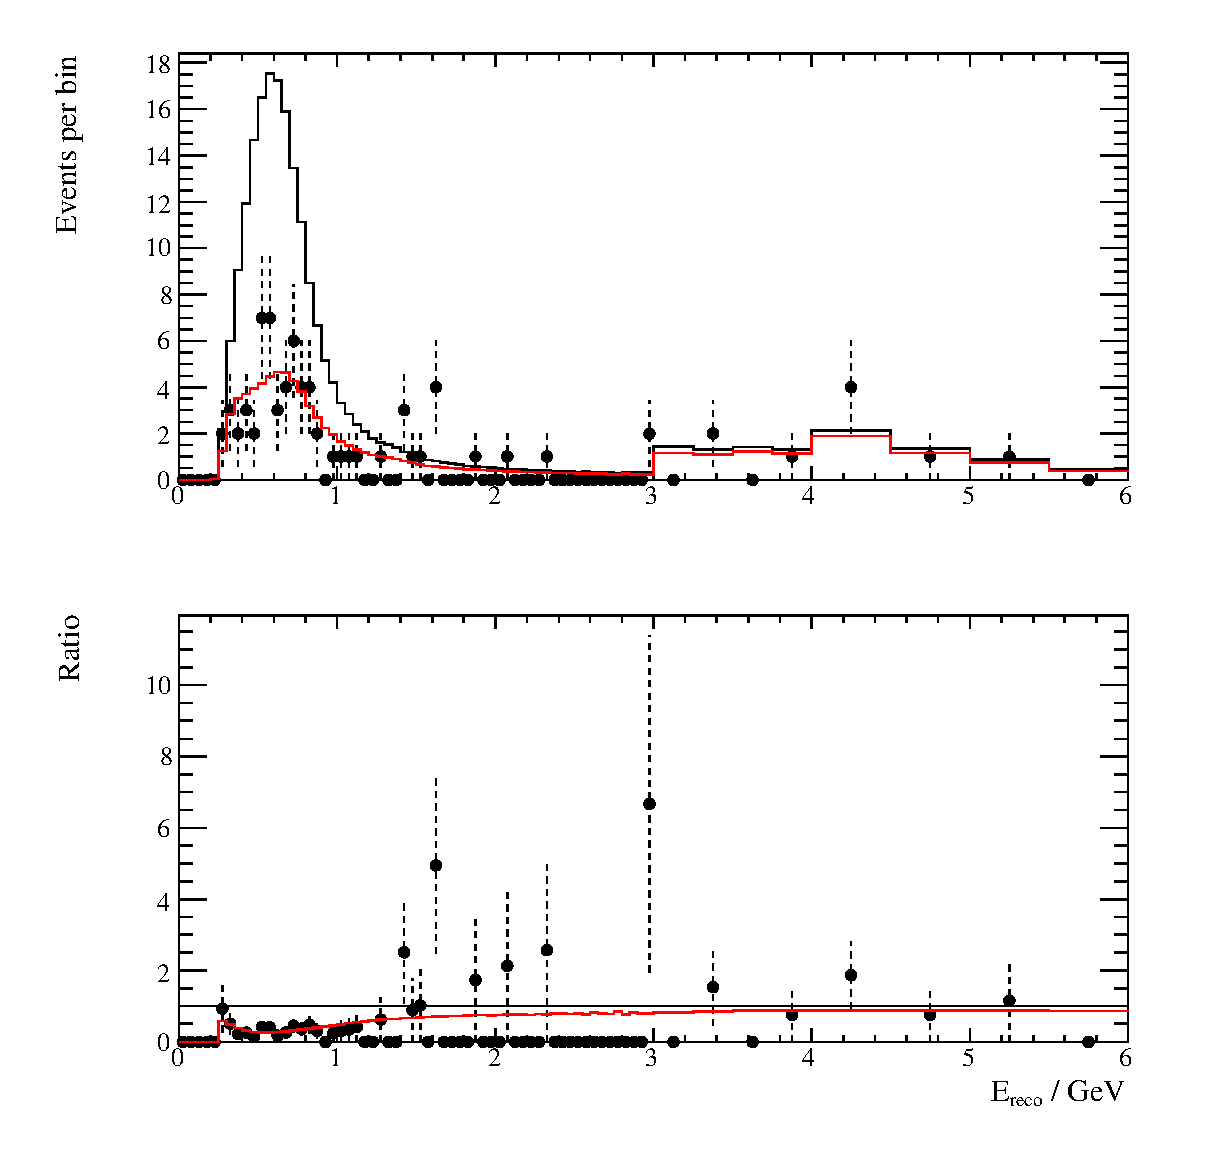
\includegraphics[width=13pc]{./images/fit_toymc/example_fits/2N/spectrum_5}
\caption { 
  Best-fit spectrum (top) and ratios of data and best-fit spectrum to predicted spectrum
  for no oscillations (bottom) for the 2+N fit to fake data set 5
}
\label{fig:fakedata_spectrum_2N_5}
\end{minipage}
\end{figure*}

%...........................................................
%
% Best-fit spectra and ratios for `2+8' fits
%

\begin{figure*}[htb]
\begin{minipage}[t]{0.48\linewidth}
\center
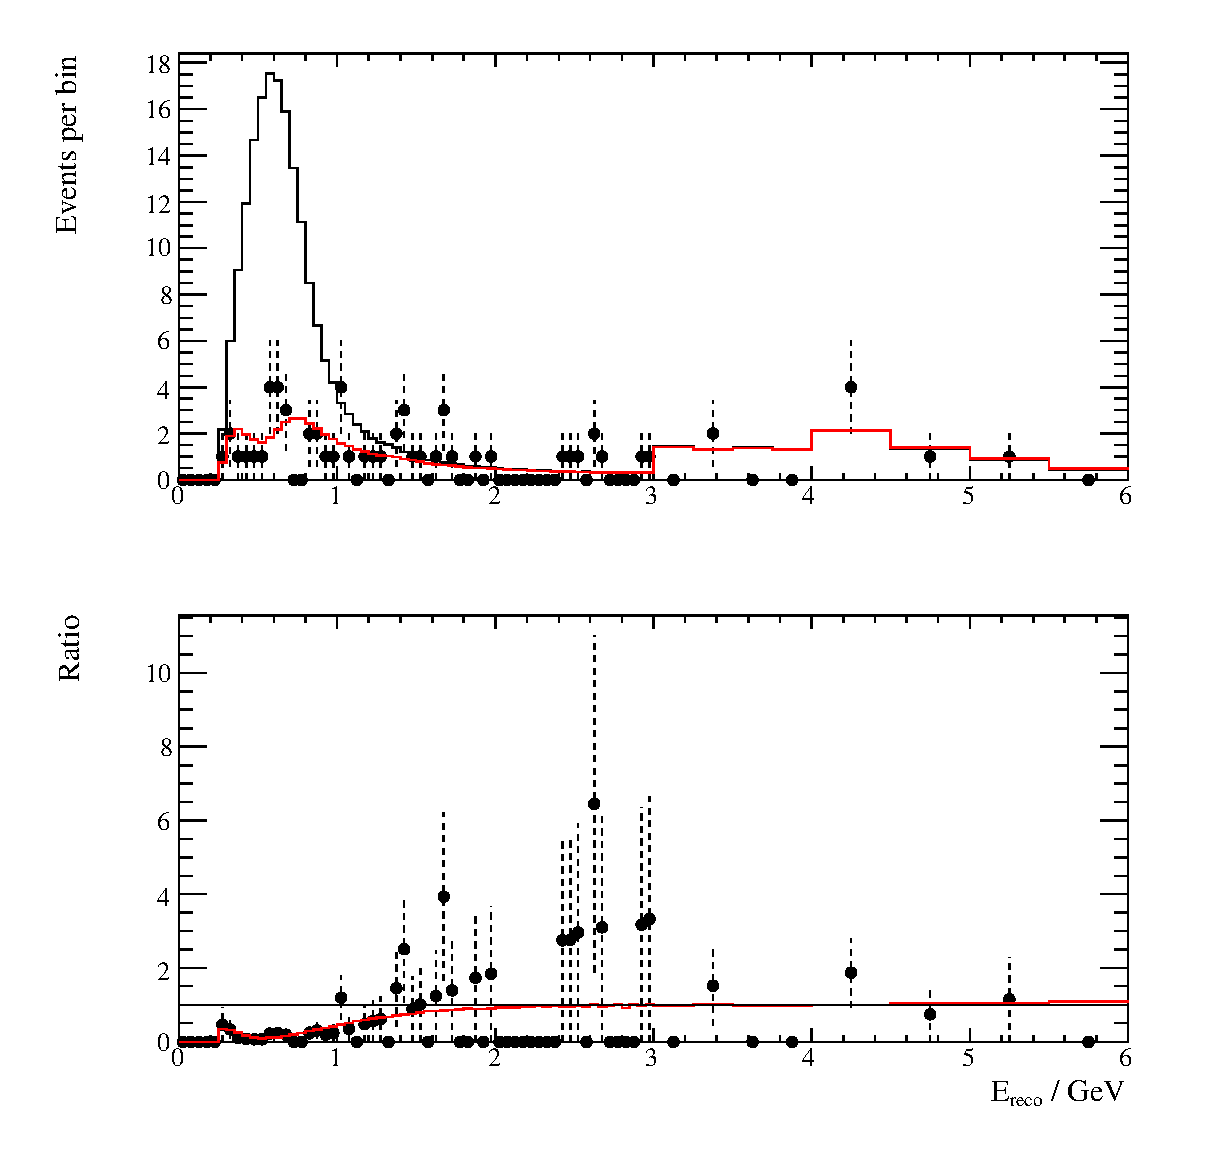
\includegraphics[width=15pc]{./images/fit_toymc/example_fits/spectrum_0}
\caption {
  Best-fit spectrum (top) and ratios of data and best-fit spectrum to predicted spectrum
  for no oscillations (bottom) for the 2+8 fit to fake data set 0
}
\label{fig:fakedata_spectrum_0}
\end{minipage}
\hspace{0.06\linewidth}
\begin{minipage}[t]{0.48\linewidth}
\center
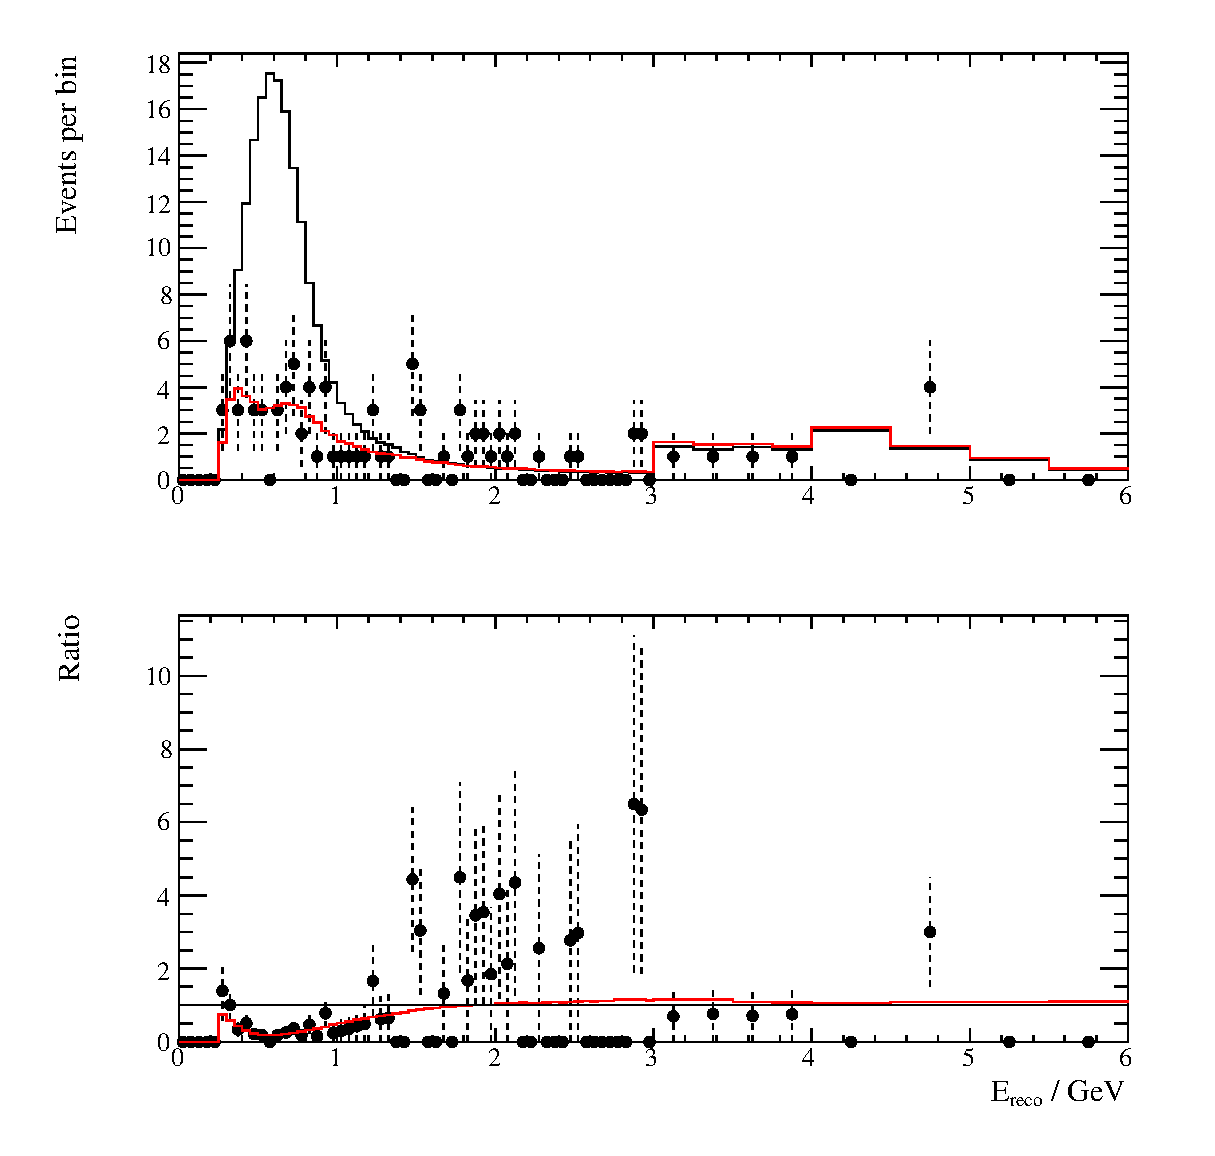
\includegraphics[width=15pc]{./images/fit_toymc/example_fits/spectrum_1}
\caption { 
  Best-fit spectrum (top) and ratios of data and best-fit spectrum to predicted spectrum
  for no oscillations (bottom) for the 2+8 fit to fake data set 1
}
\label{fig:fakedata_spectrum_1}
\end{minipage}
\vfill
\begin{minipage}[t]{0.48\linewidth}
\center
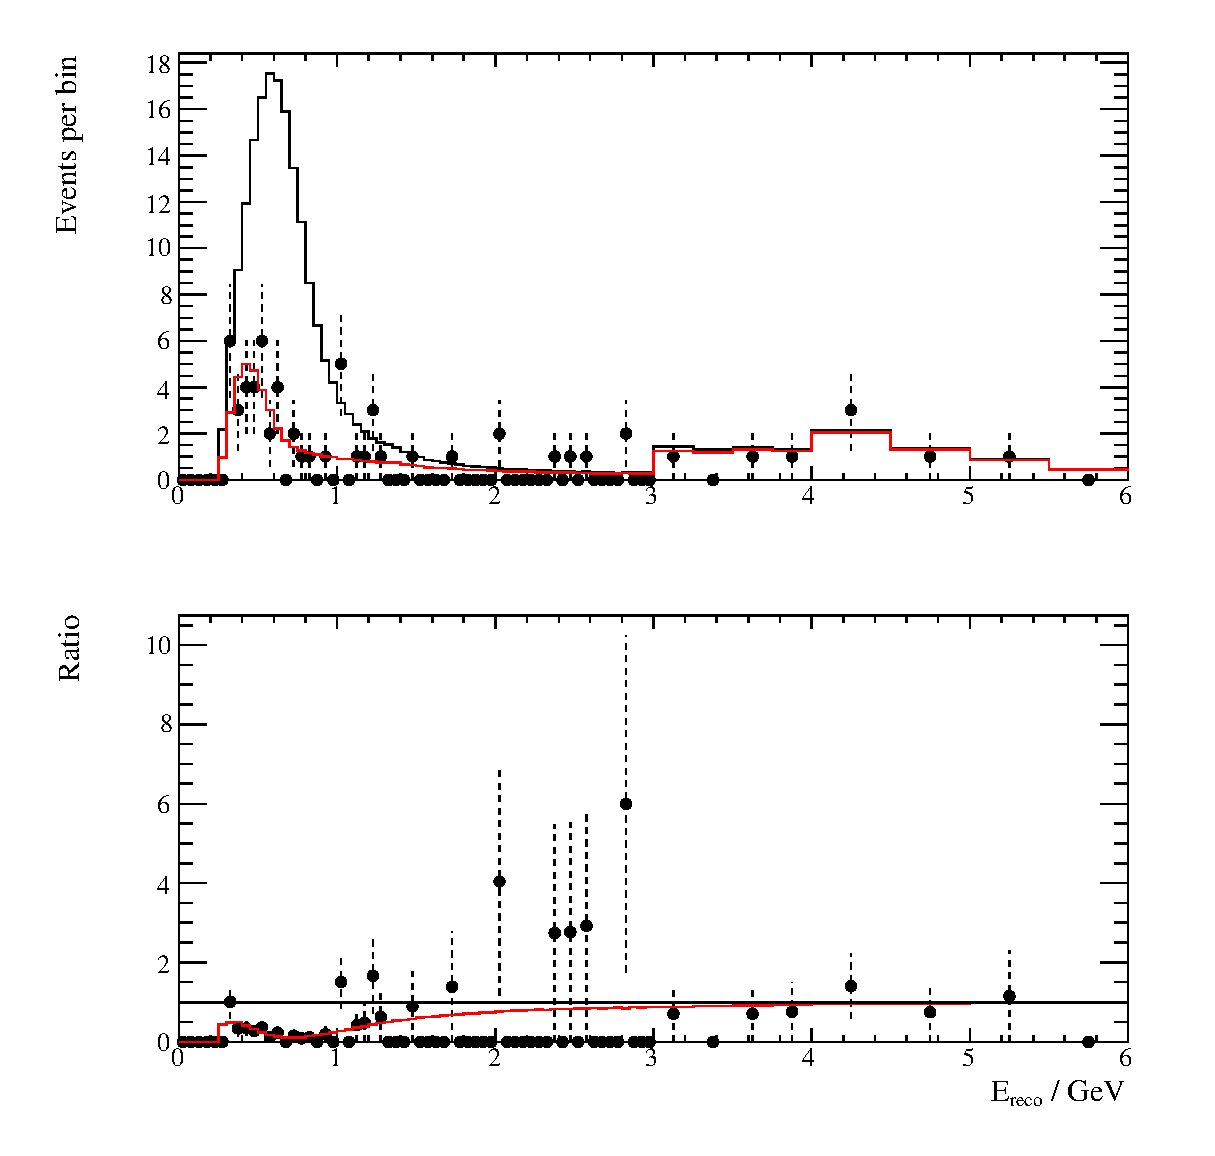
\includegraphics[width=15pc]{./images/fit_toymc/example_fits/spectrum_2}
\caption {
  Best-fit spectrum (top) and ratios of data and best-fit spectrum to predicted spectrum
  for no oscillations (bottom) for the 2+8 fit to fake data set 2
}
\label{fig:fakedata_spectrum_2}
\end{minipage}
\hspace{0.06\linewidth}
\begin{minipage}[t]{0.48\linewidth}
\center
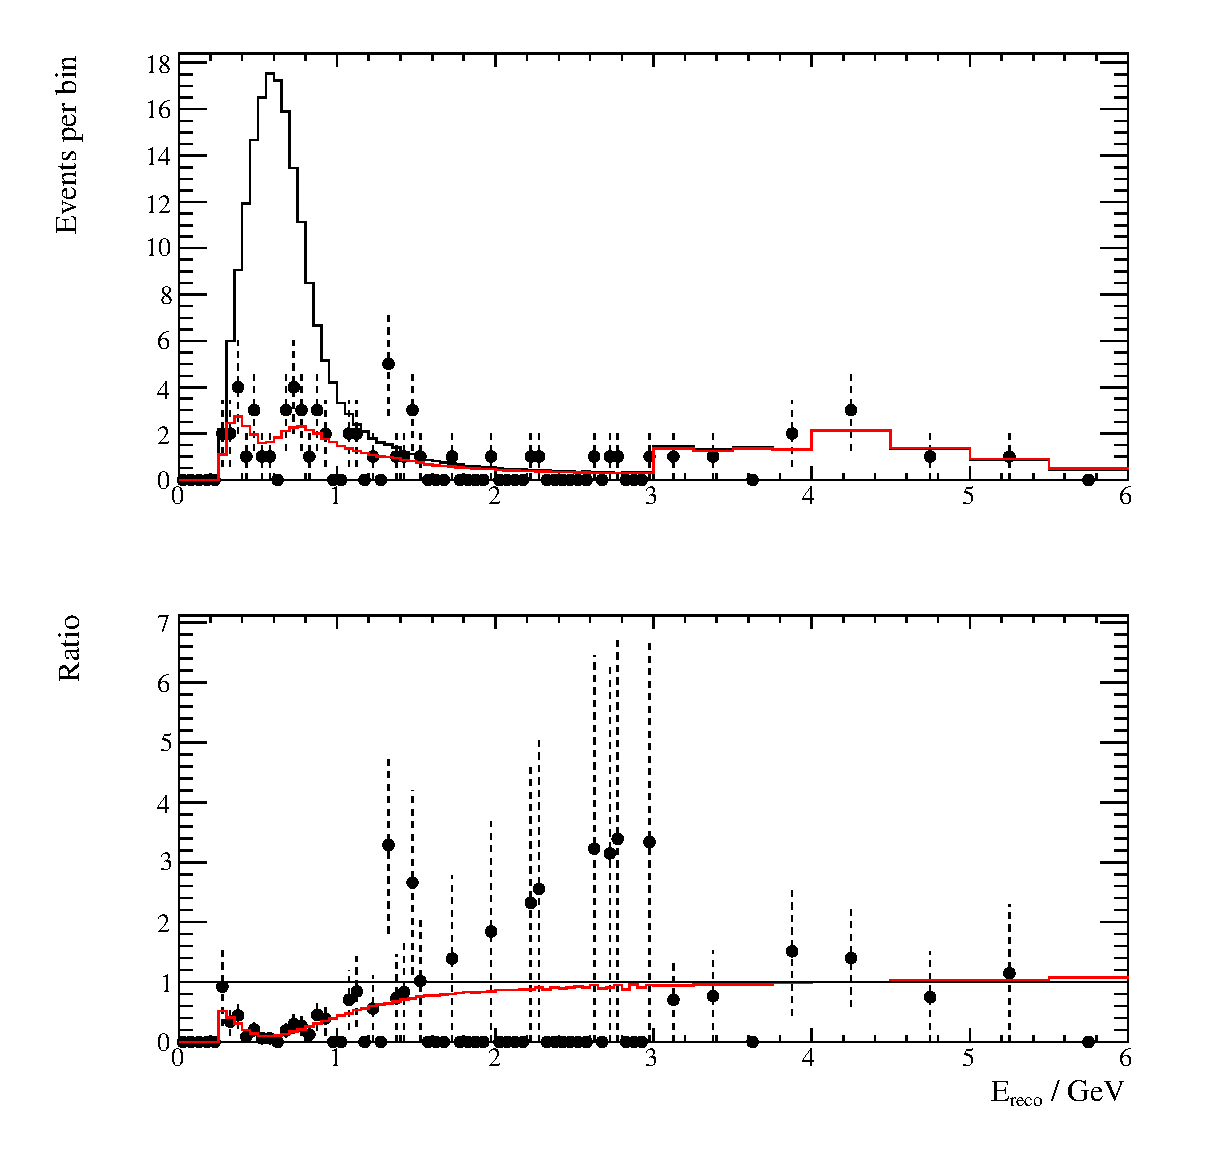
\includegraphics[width=15pc]{./images/fit_toymc/example_fits/spectrum_3}
\caption { 
  Best-fit spectrum (top) and ratios of data and best-fit spectrum to predicted spectrum
  for no oscillations (bottom) for the 2+8 fit to fake data set 3
}
\label{fig:fakedata_spectrum_3}
\end{minipage}
\vfill
\begin{minipage}[t]{0.48\linewidth}
\center
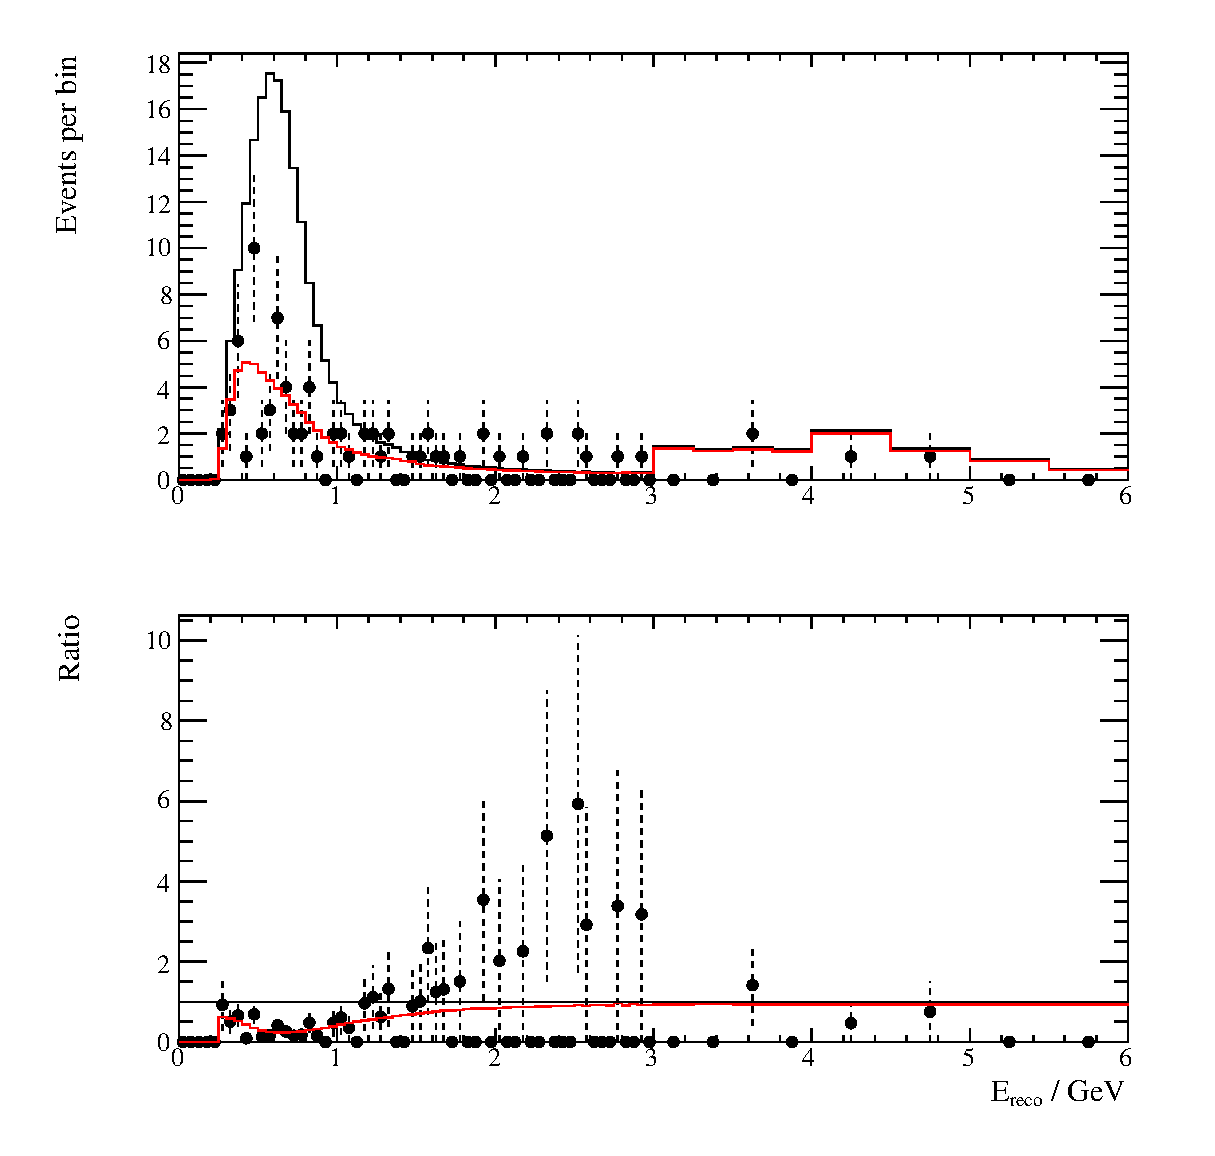
\includegraphics[width=15pc]{./images/fit_toymc/example_fits/spectrum_4}
\caption {
  Best-fit spectrum (top) and ratios of data and best-fit spectrum to predicted spectrum
  for no oscillations (bottom) for the 2+8 fit to fake data set 4
}
\label{fig:fakedata_spectrum_4}
\end{minipage}
\hspace{0.06\linewidth}
\begin{minipage}[t]{0.48\linewidth}
\center
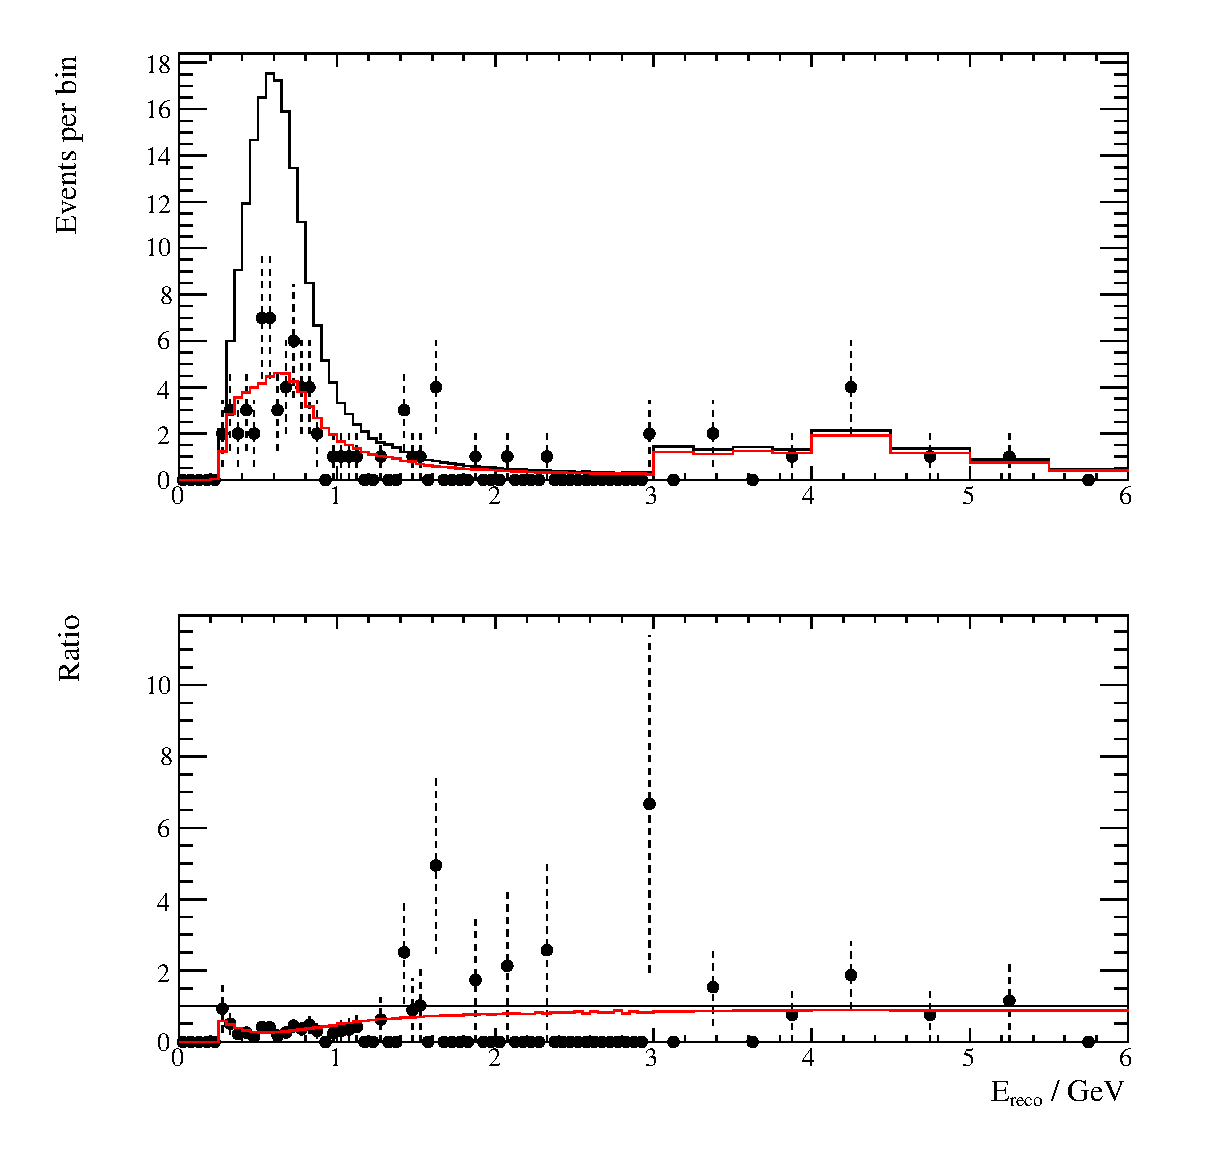
\includegraphics[width=15pc]{./images/fit_toymc/example_fits/spectrum_5}
\caption { 
  Best-fit spectrum (top) and ratios of data and best-fit spectrum to predicted spectrum
  for no oscillations (bottom) for the 2+8 fit to fake data set 5
}
\label{fig:fakedata_spectrum_5}
\end{minipage}
\end{figure*}

%...........................................................
%
% Best-fit spectra comparison comparing 2+8, 2+N and input
%

\begin{figure*}[htb]
\begin{minipage}[t]{0.48\linewidth}
\center
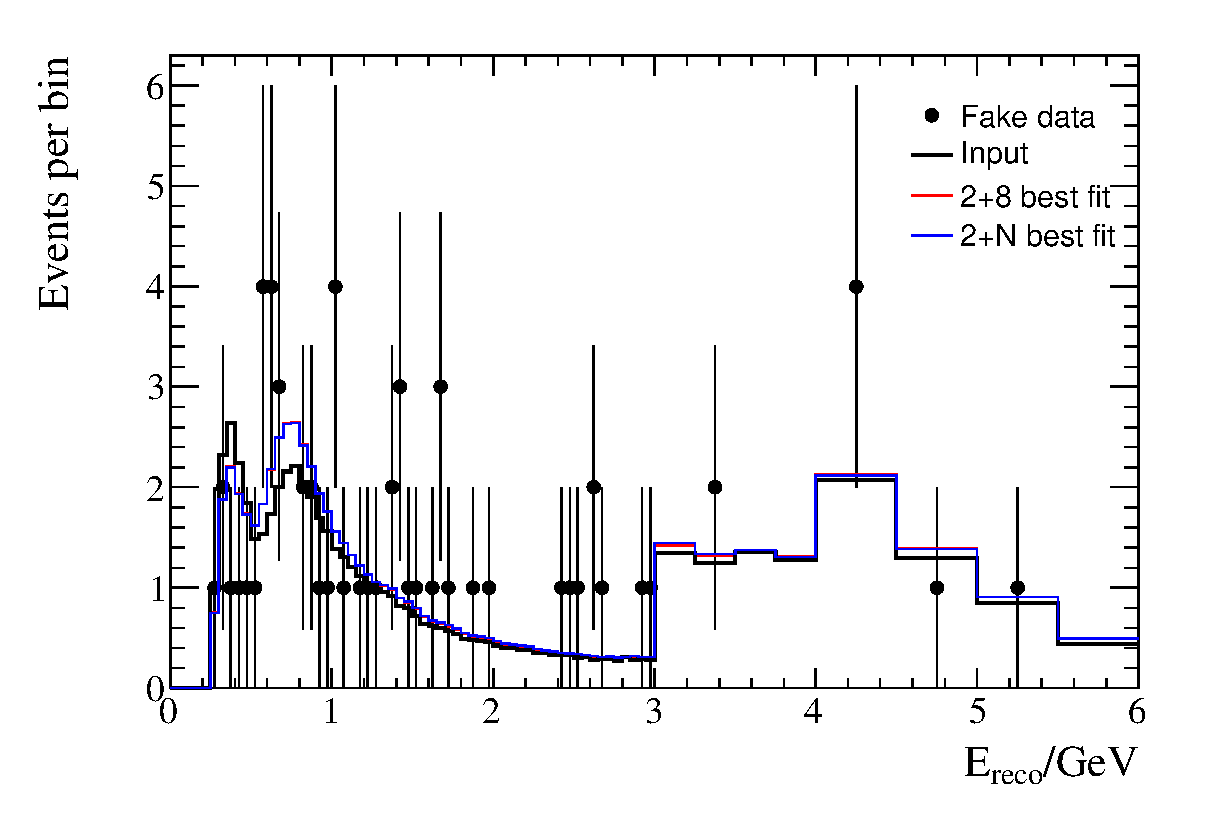
\includegraphics[width=18pc]{./images/fit_toymc/example_fits/fakedata_spectra_comparison_0}
\caption {
  Comparisons of the 2+8 and 2+N best-fit spectra with the input distribution for fake data set 0
}
\label{fig:fakedata_spectrum_comparison_0}
\end{minipage}
\hspace{0.06\linewidth}
\begin{minipage}[t]{0.48\linewidth}
\center
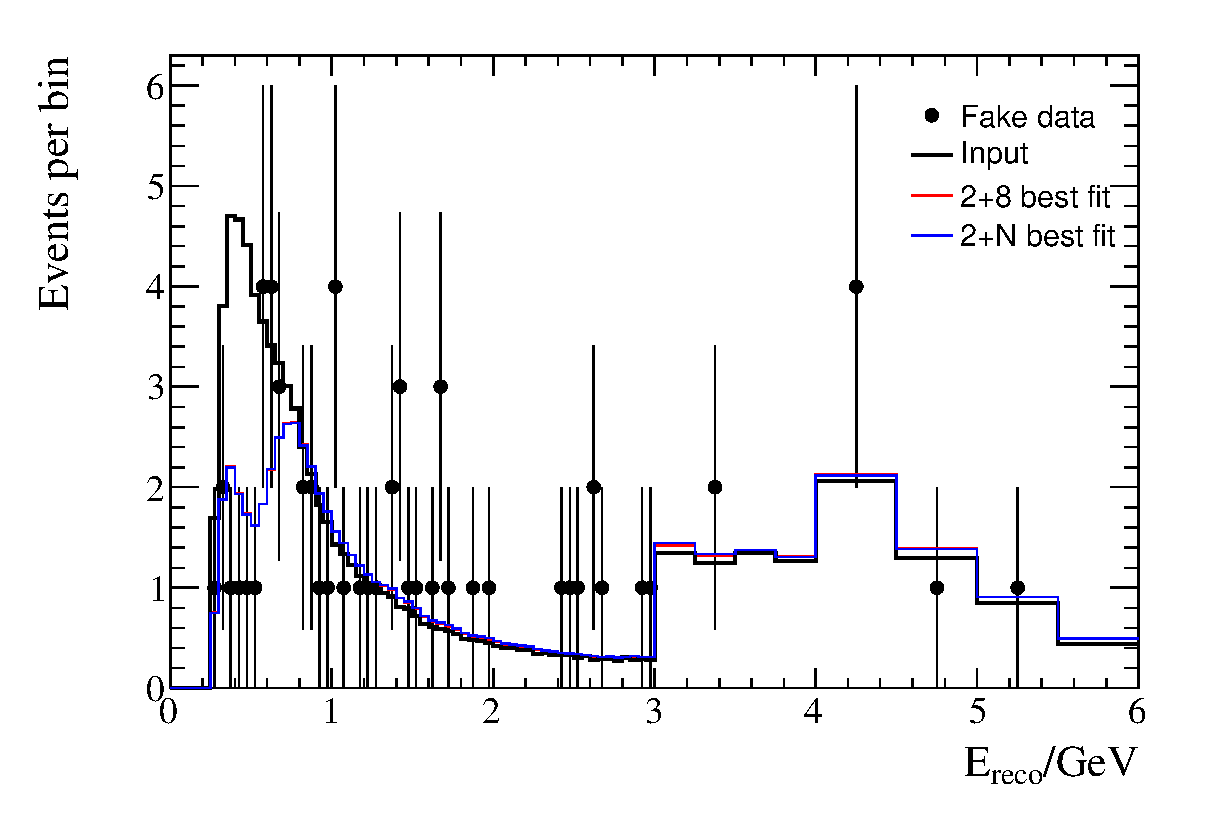
\includegraphics[width=18pc]{./images/fit_toymc/example_fits/fakedata_spectra_comparison_1}
\caption { 
  Comparisons of the 2+8 and 2+N best-fit spectra with the input distribution for fake data set 1
}
\label{fig:fakedata_spectrum_comparison_1}
\end{minipage}
\vfill
\begin{minipage}[t]{0.48\linewidth}
\center
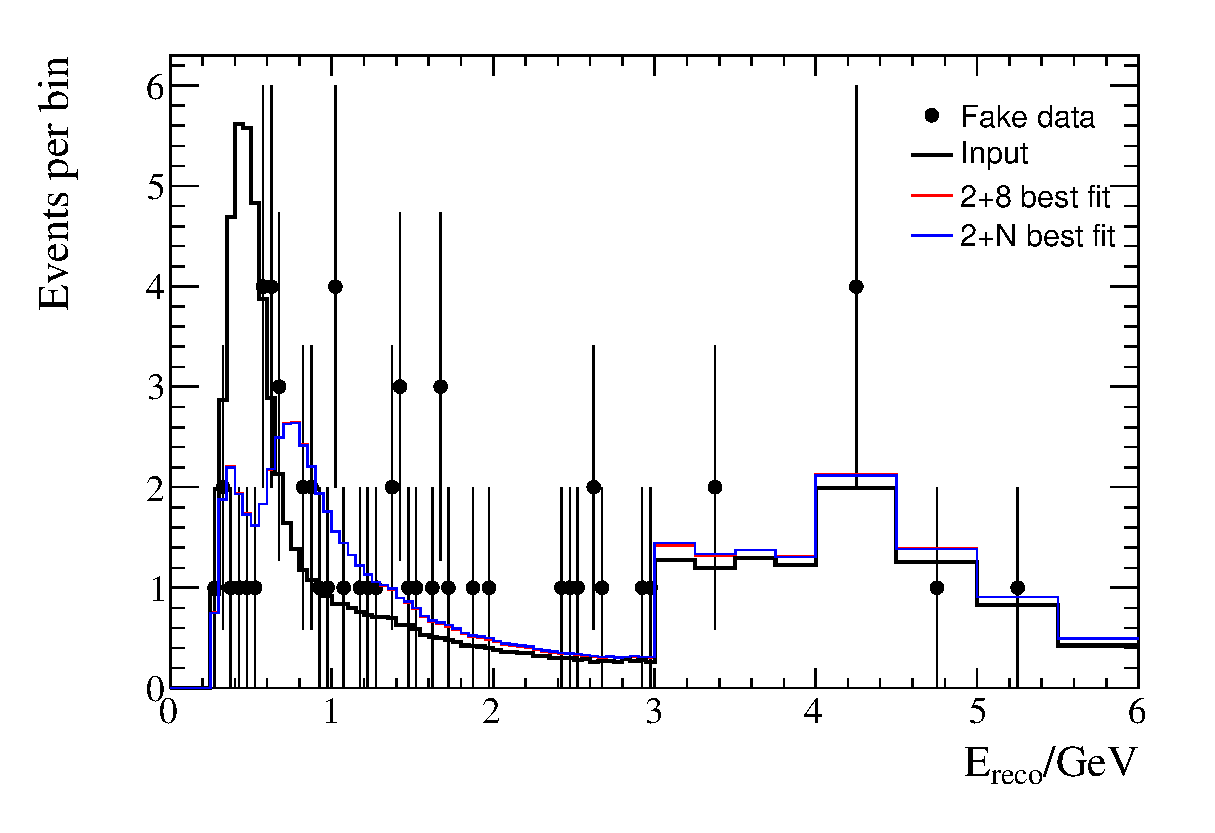
\includegraphics[width=18pc]{./images/fit_toymc/example_fits/fakedata_spectra_comparison_2}
\caption {
  Comparisons of the 2+8 and 2+N best-fit spectra with the input distribution for fake data set 2
}
\label{fig:fakedata_spectrum_comparison_2}
\end{minipage}
\hspace{0.06\linewidth}
\begin{minipage}[t]{0.48\linewidth}
\center
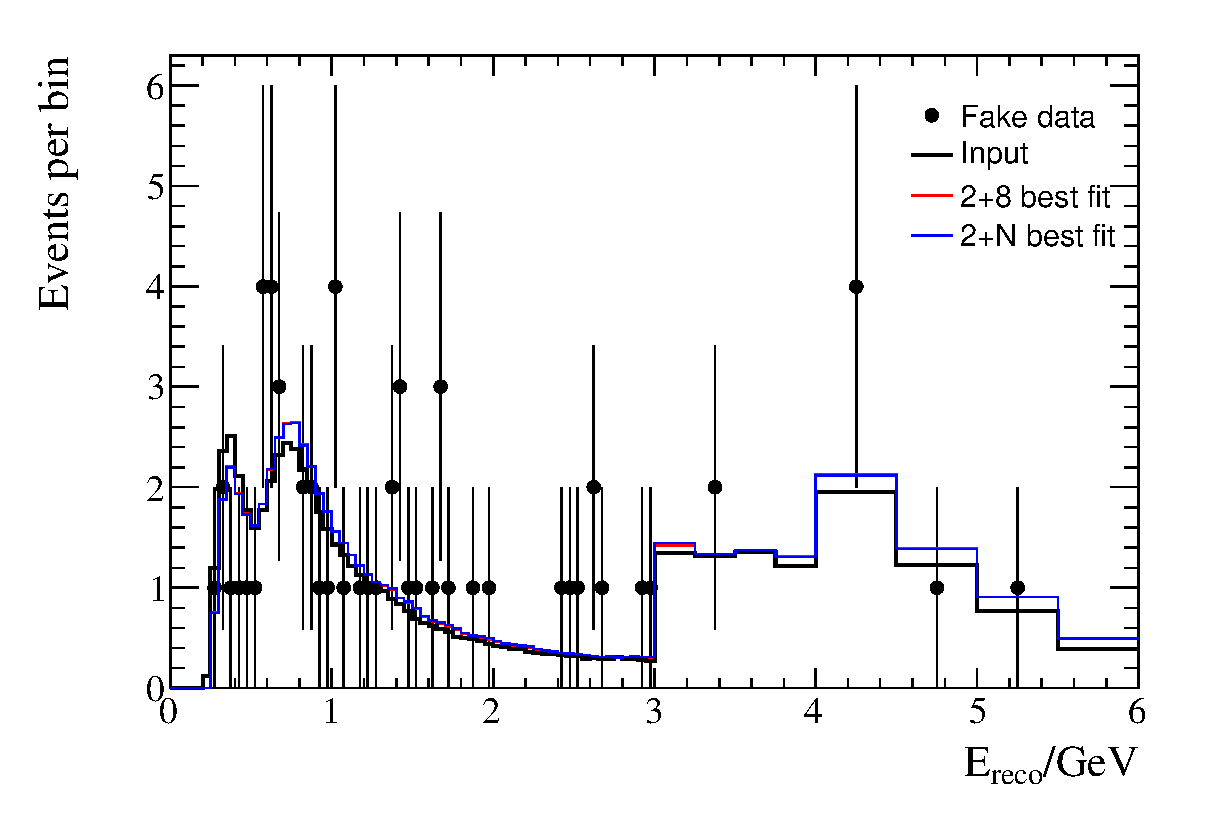
\includegraphics[width=18pc]{./images/fit_toymc/example_fits/fakedata_spectra_comparison_3}
\caption { 
  Comparisons of the 2+8 and 2+N best-fit spectra with the input distribution for fake data set 3
}
\label{fig:fakedata_spectrum_comparison_3}
\end{minipage}
\vfill
\begin{minipage}[t]{0.48\linewidth}
\center
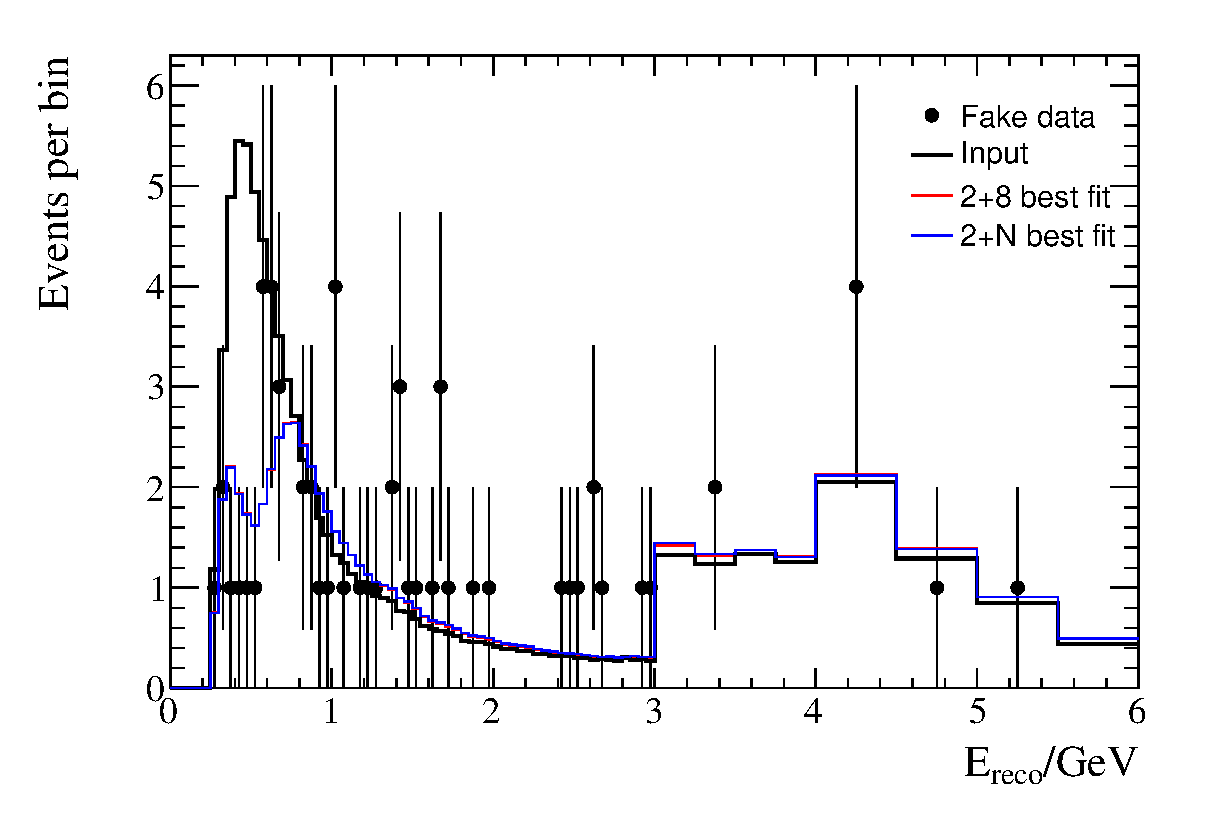
\includegraphics[width=18pc]{./images/fit_toymc/example_fits/fakedata_spectra_comparison_4}
\caption {
  Comparisons of the 2+8 and 2+N best-fit spectra with the input distribution for fake data set 4
}
\label{fig:fakedata_spectrum_comparison_4}
\end{minipage}
\hspace{0.06\linewidth}
\begin{minipage}[t]{0.48\linewidth}
\center
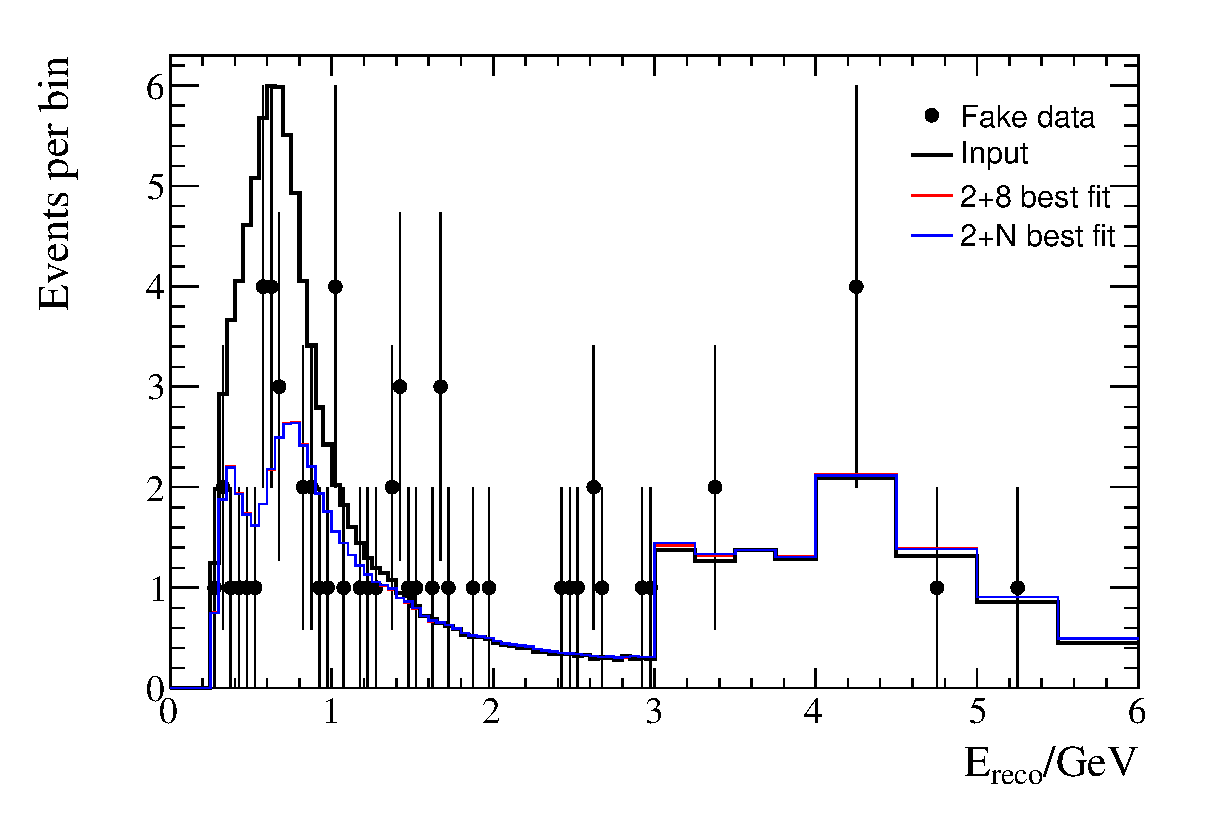
\includegraphics[width=18pc]{./images/fit_toymc/example_fits/fakedata_spectra_comparison_5}
\caption { 
  Comparisons of the 2+8 and 2+N best-fit spectra with the input distribution for fake data set 5
}
\label{fig:fakedata_spectrum_comparison_5}
\end{minipage}
\end{figure*}

\clearpage
\subsection{$\Delta\chi^2$ surfaces}
\label{appendix:example_toy_mc_fits:dchisq}

%...........................................................
%
% dchisq surfaces for `2+N' fits
%

\begin{figure*}[htb]
\begin{minipage}[t]{0.48\linewidth}
\center
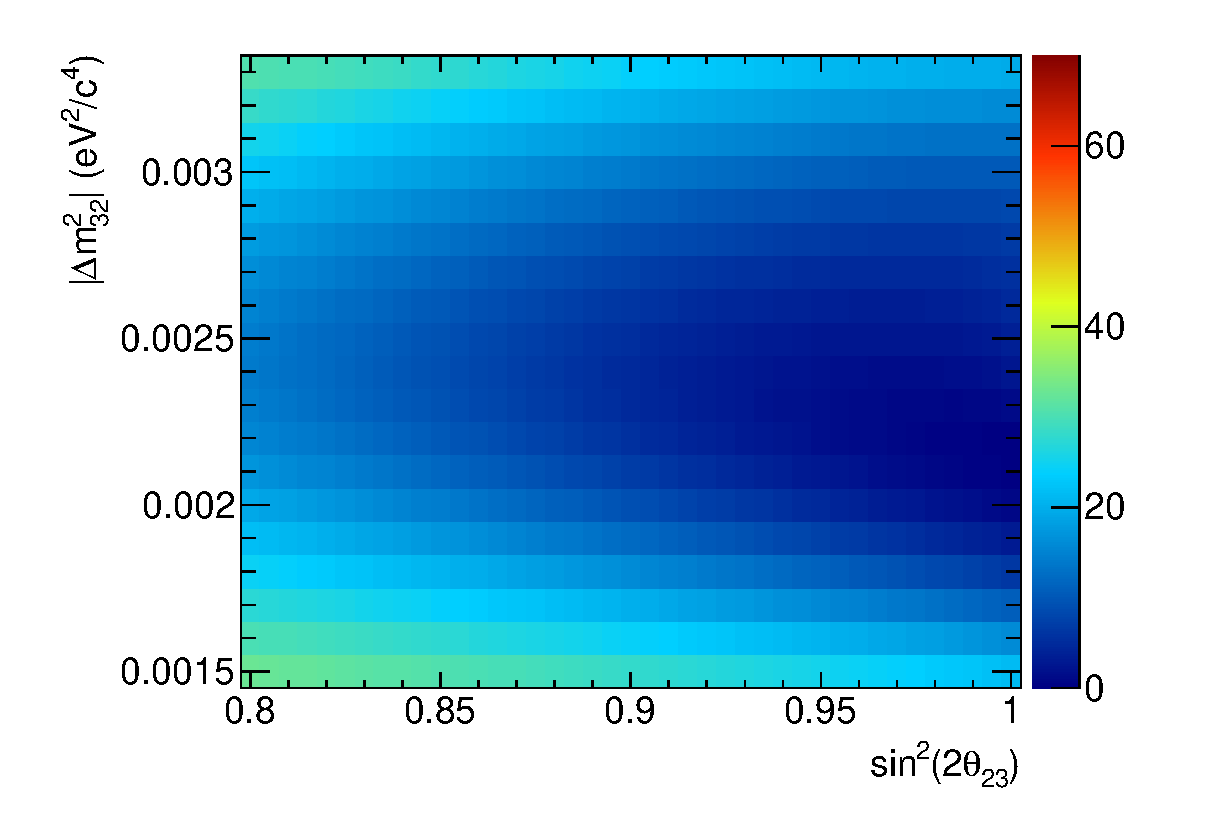
\includegraphics[width=18pc]{./images/fit_toymc/example_fits/2N/dchisq_0}
\caption {
  $\Delta\chi^2$ surface for the 2+N fit to fake data set 0
}
\label{fig:fakedata_chisq_2N_0}
\end{minipage}
\hspace{0.06\linewidth}
\begin{minipage}[t]{0.48\linewidth}
\center
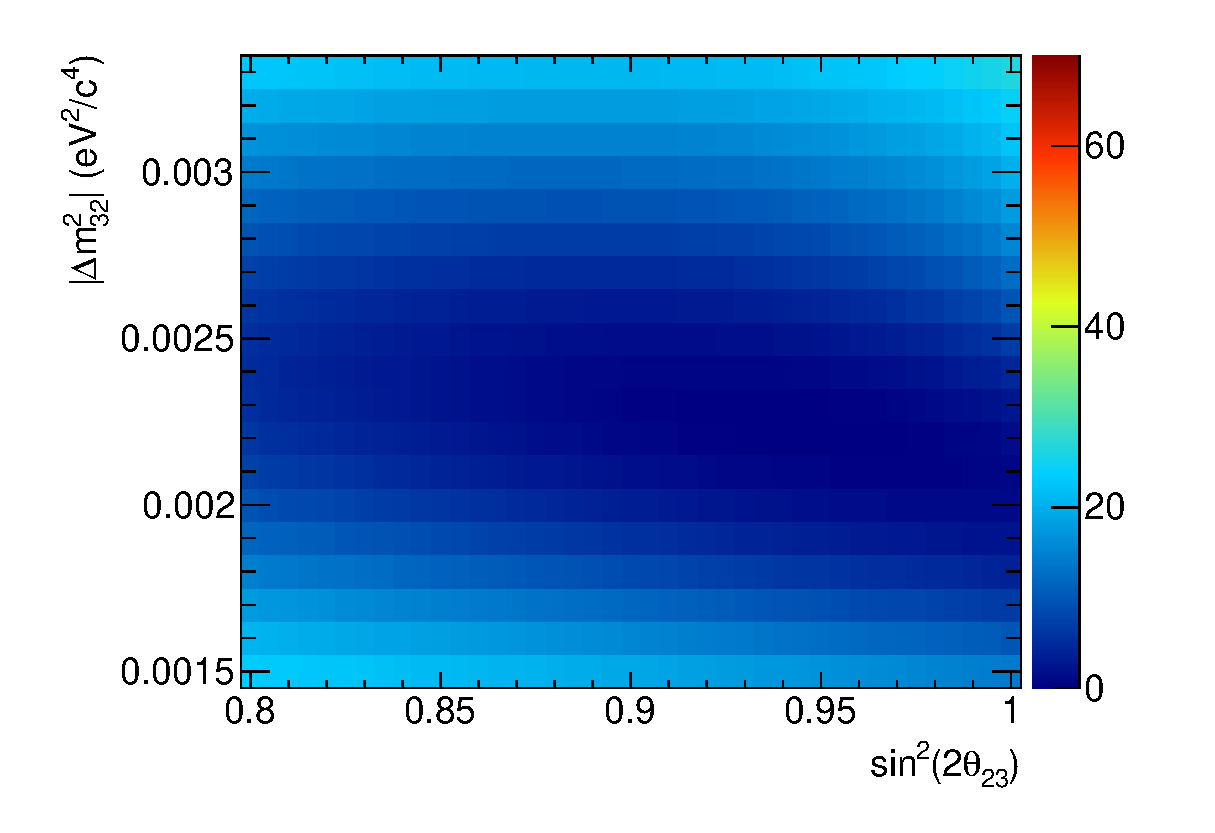
\includegraphics[width=18pc]{./images/fit_toymc/example_fits/2N/dchisq_1}
\caption { 
  $\Delta\chi^2$ surface for the 2+N fit to fake data set 1
}
\label{fig:fakedata_chisq_2N_1}
\end{minipage}
\vfill
\begin{minipage}[t]{0.48\linewidth}
\center
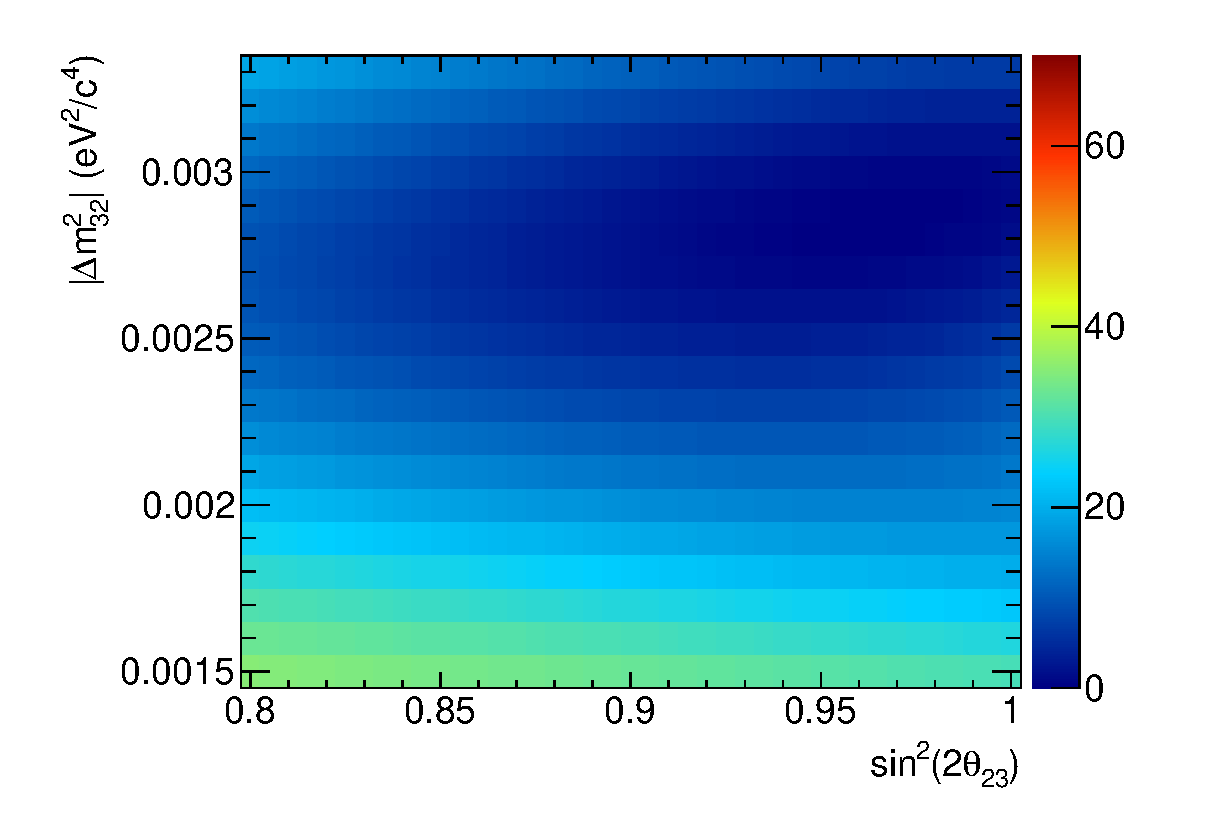
\includegraphics[width=18pc]{./images/fit_toymc/example_fits/2N/dchisq_2}
\caption {
  $\Delta\chi^2$ surface for the 2+N fit to fake data set 2
}
\label{fig:fakedata_chisq_2N_2}
\end{minipage}
\hspace{0.06\linewidth}
\begin{minipage}[t]{0.48\linewidth}
\center
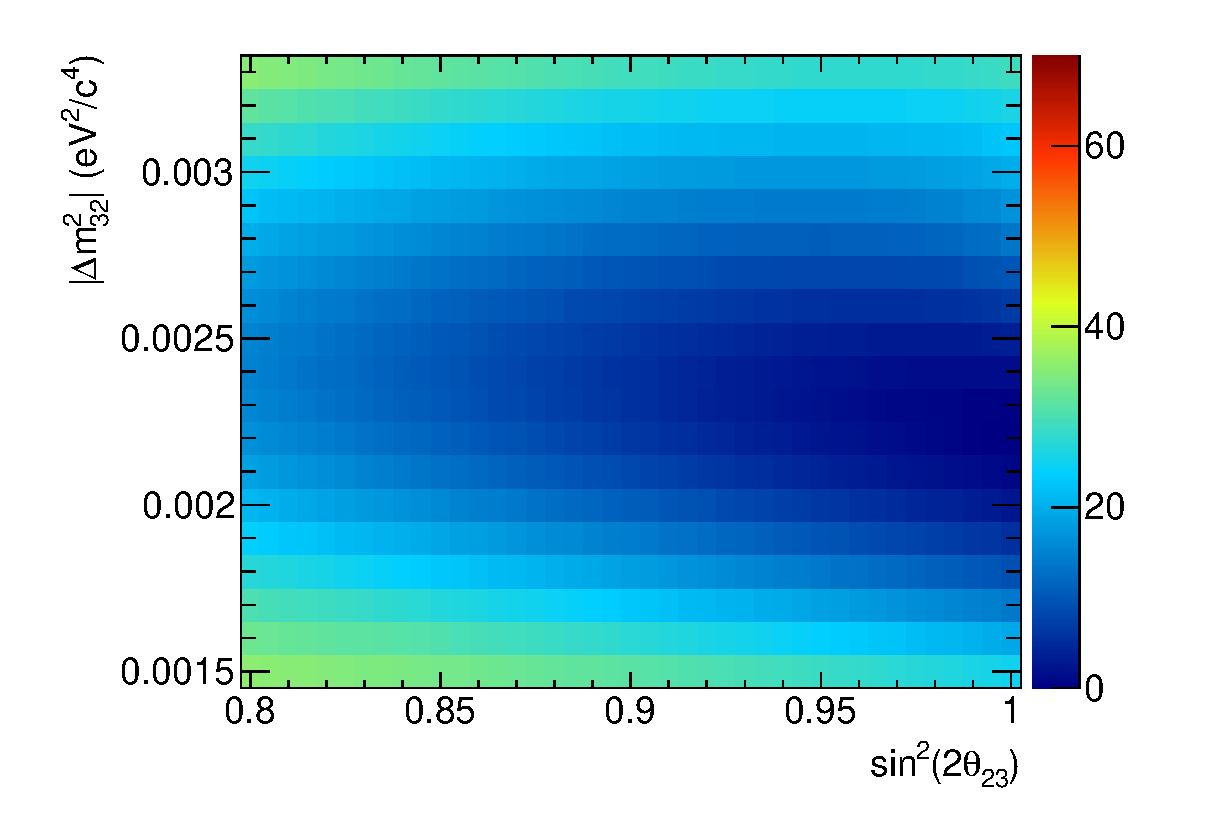
\includegraphics[width=18pc]{./images/fit_toymc/example_fits/2N/dchisq_3}
\caption { 
  $\Delta\chi^2$ surface for the 2+N fit to fake data set 3
}
\label{fig:fakedata_chisq_2N_3}
\end{minipage}
\vfill
\begin{minipage}[t]{0.48\linewidth}
\center
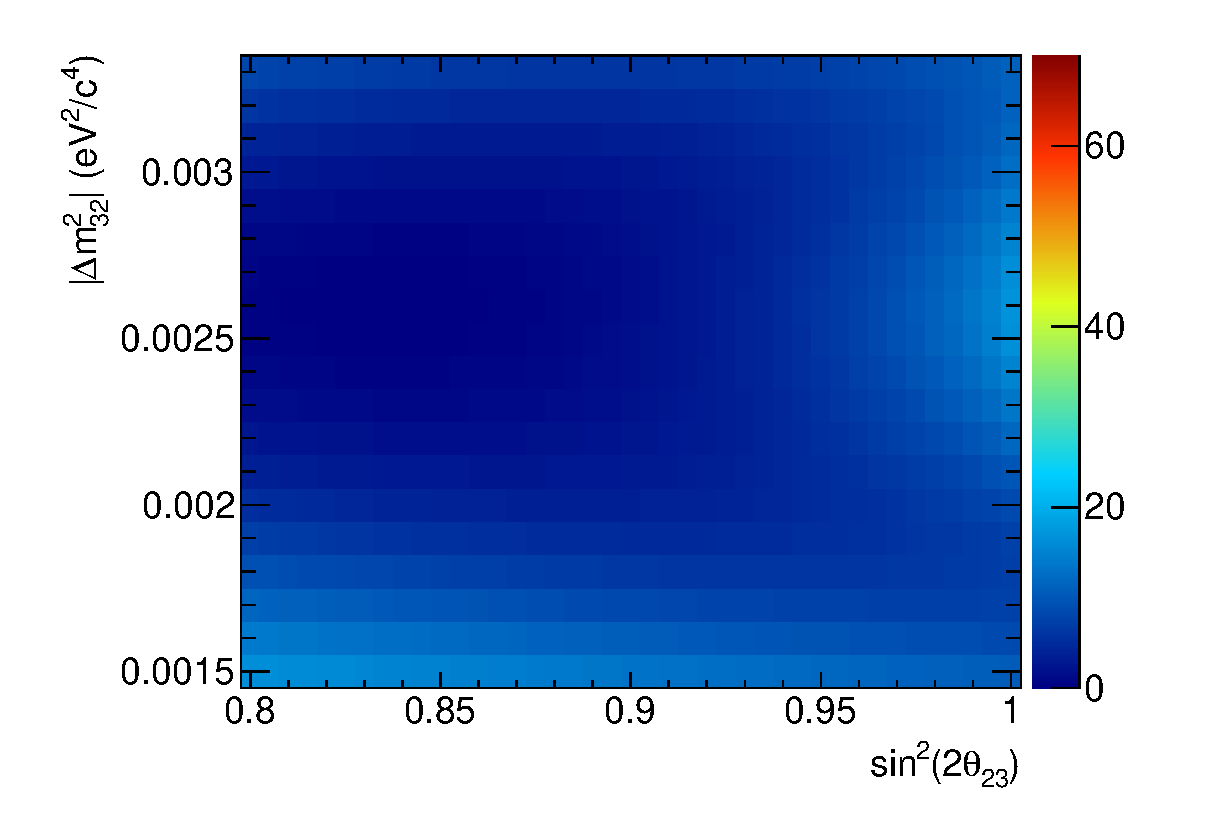
\includegraphics[width=18pc]{./images/fit_toymc/example_fits/2N/dchisq_4}
\caption {
  $\Delta\chi^2$ surface for the 2+N fit to fake data set 4
}
\label{fig:fakedata_chisq_2N_4}
\end{minipage}
\hspace{0.06\linewidth}
\begin{minipage}[t]{0.48\linewidth}
\center
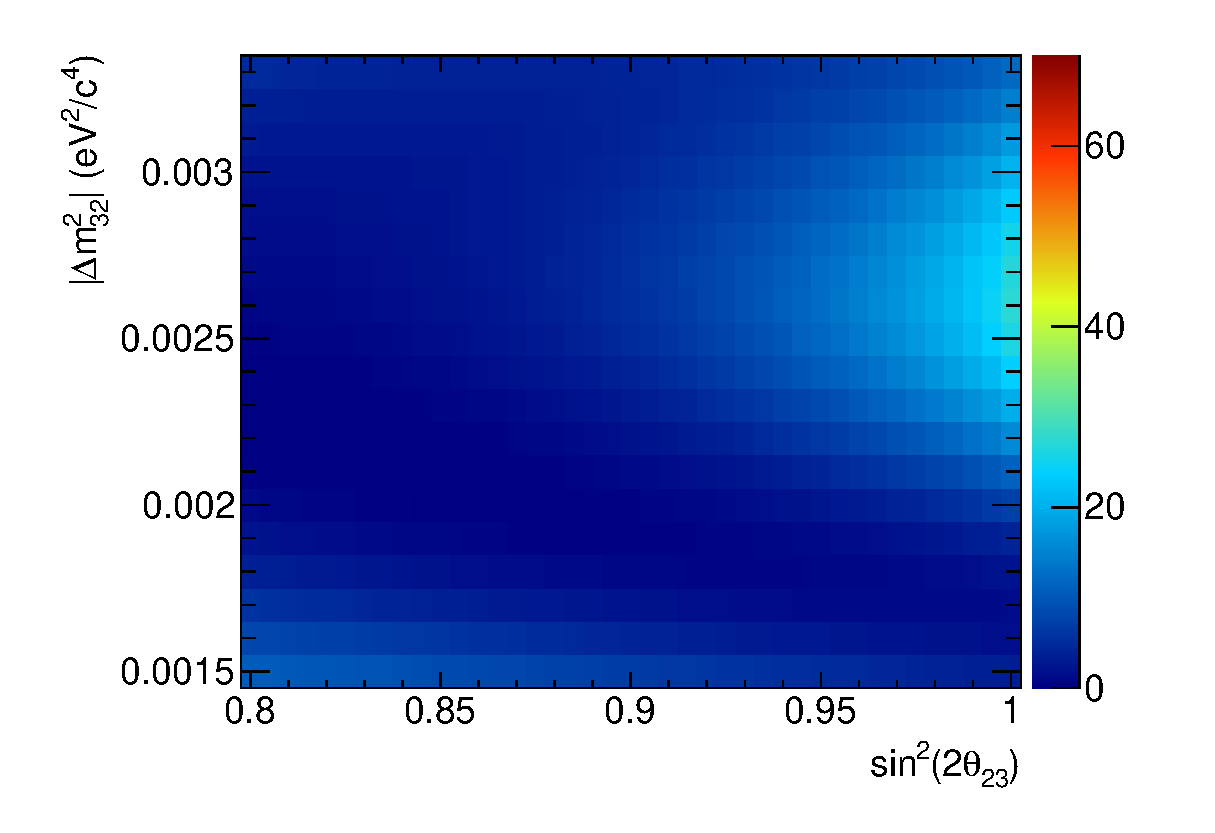
\includegraphics[width=18pc]{./images/fit_toymc/example_fits/2N/dchisq_5}
\caption { 
  $\Delta\chi^2$ surface for the 2+N fit to fake data set 5
}
\label{fig:fakedata_chisq_2N_5}
\end{minipage}
\end{figure*}

%...........................................................
%
% dchisq surfaces for `2+8' fits
%

\begin{figure*}[htb]
\begin{minipage}[t]{0.48\linewidth}
\center
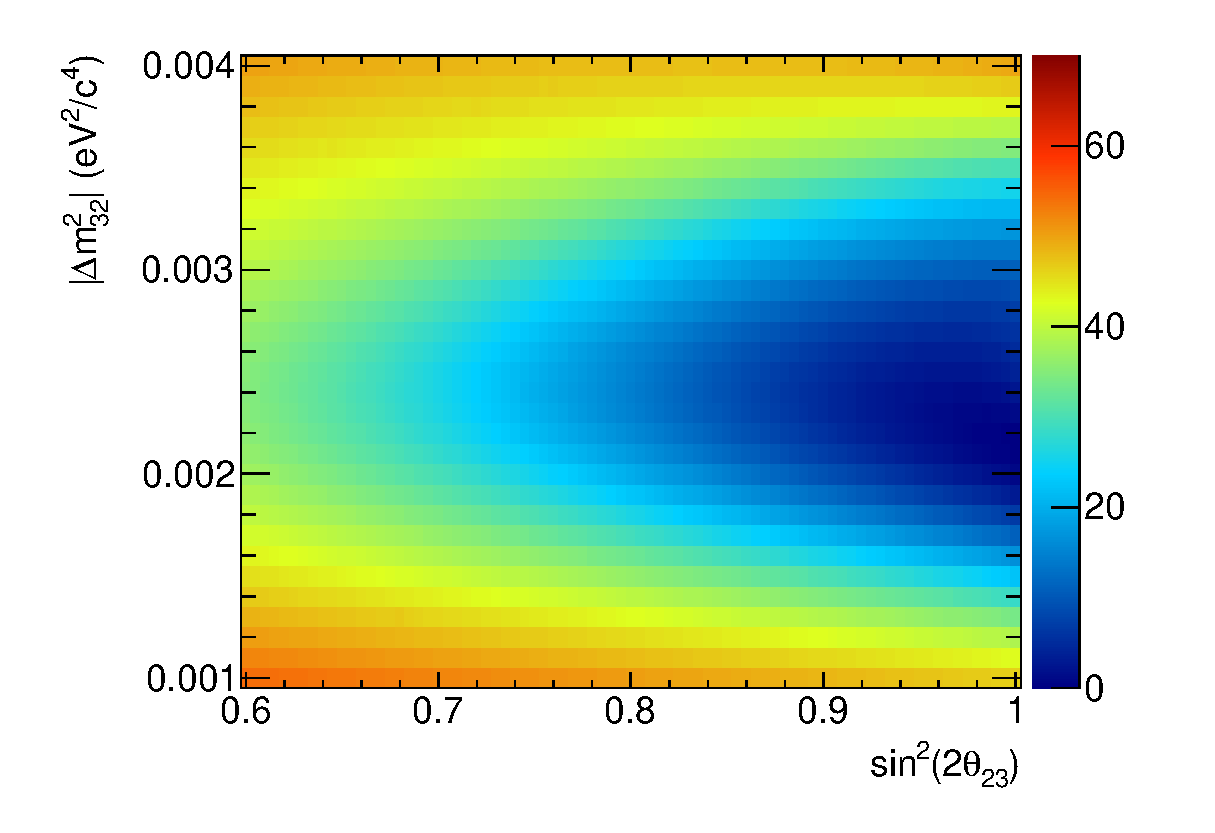
\includegraphics[width=18pc]{./images/fit_toymc/example_fits/dchisq_0}
\caption {
  $\Delta\chi^2$ surface for the 2+8 fit to fake data set 0
}
\label{fig:fakedata_chisq_0}
\end{minipage}
\hspace{0.06\linewidth}
\begin{minipage}[t]{0.48\linewidth}
\center
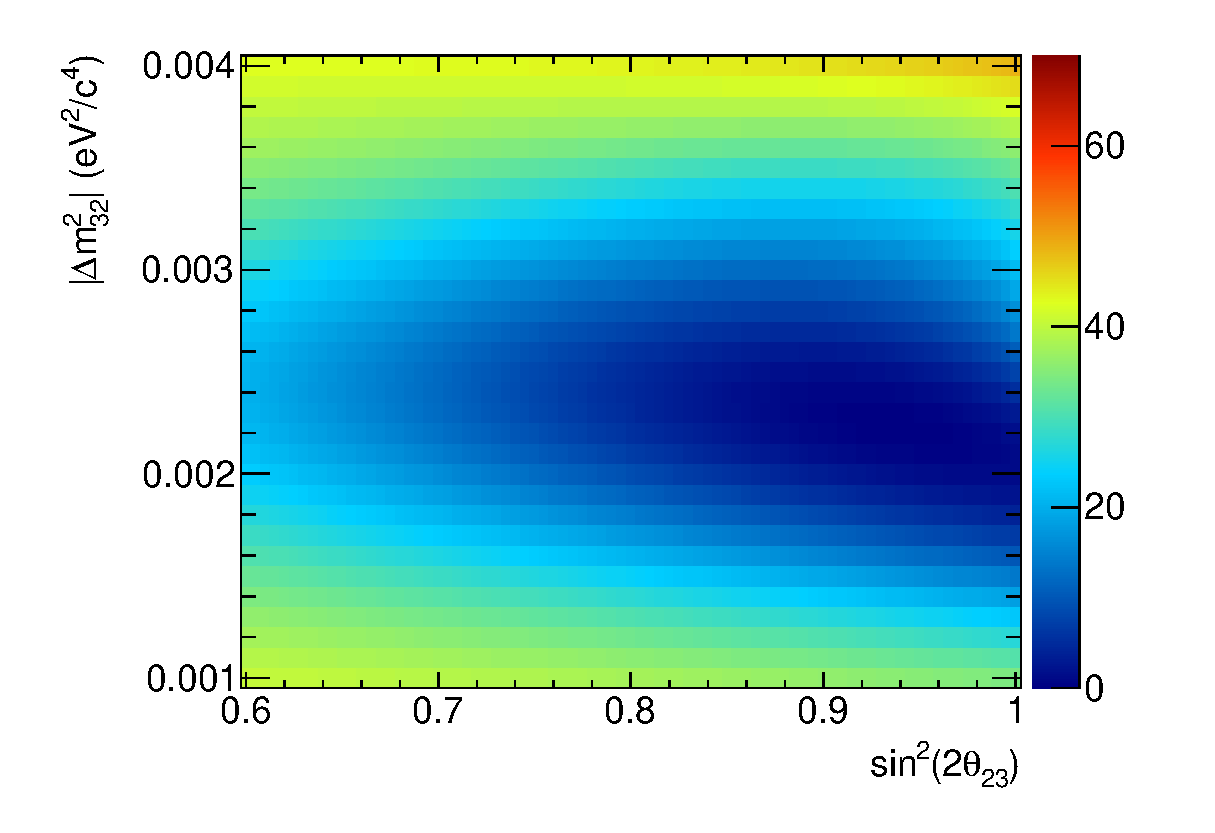
\includegraphics[width=18pc]{./images/fit_toymc/example_fits/dchisq_1}
\caption { 
  $\Delta\chi^2$ surface for the 2+8 fit to fake data set 1
}
\label{fig:fakedata_chisq_1}
\end{minipage}
\vfill
\begin{minipage}[t]{0.48\linewidth}
\center
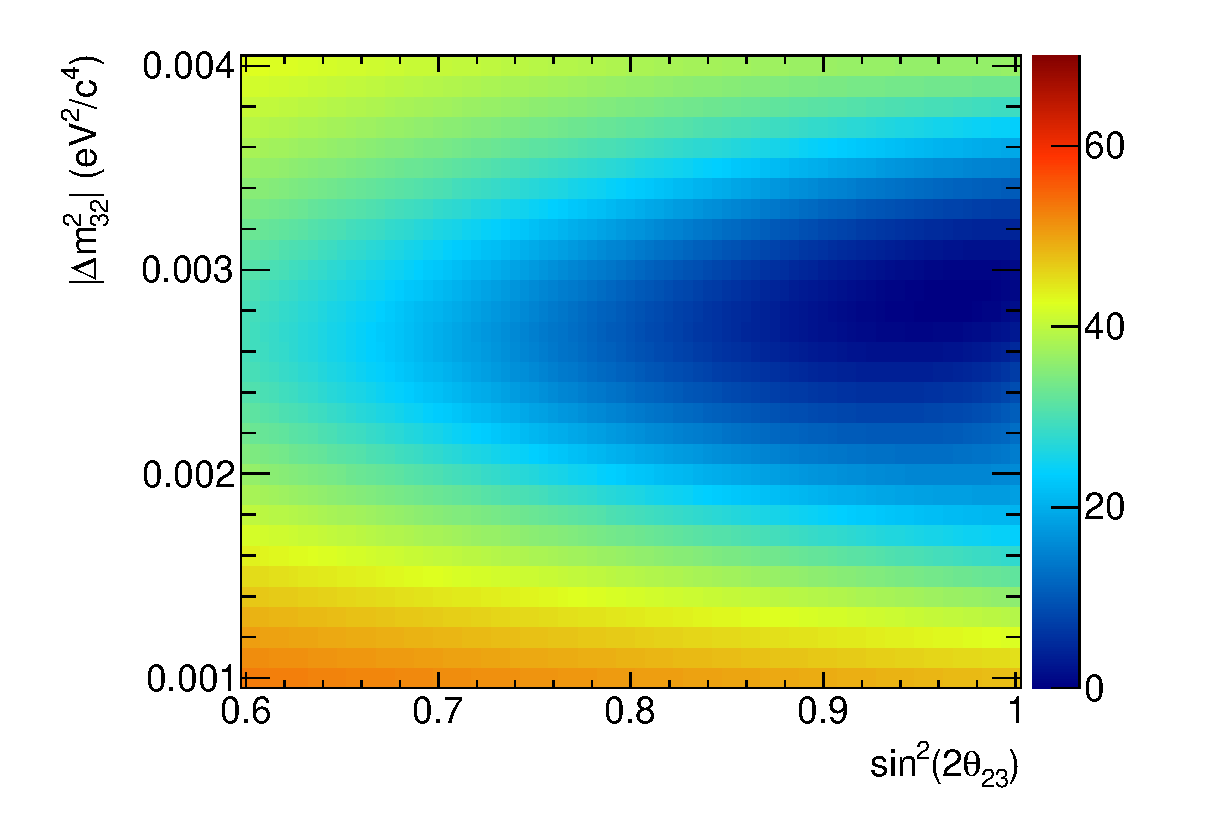
\includegraphics[width=18pc]{./images/fit_toymc/example_fits/dchisq_2}
\caption {
  $\Delta\chi^2$ surface for the 2+8 fit to fake data set 2
}
\label{fig:fakedata_chisq_2}
\end{minipage}
\hspace{0.06\linewidth}
\begin{minipage}[t]{0.48\linewidth}
\center
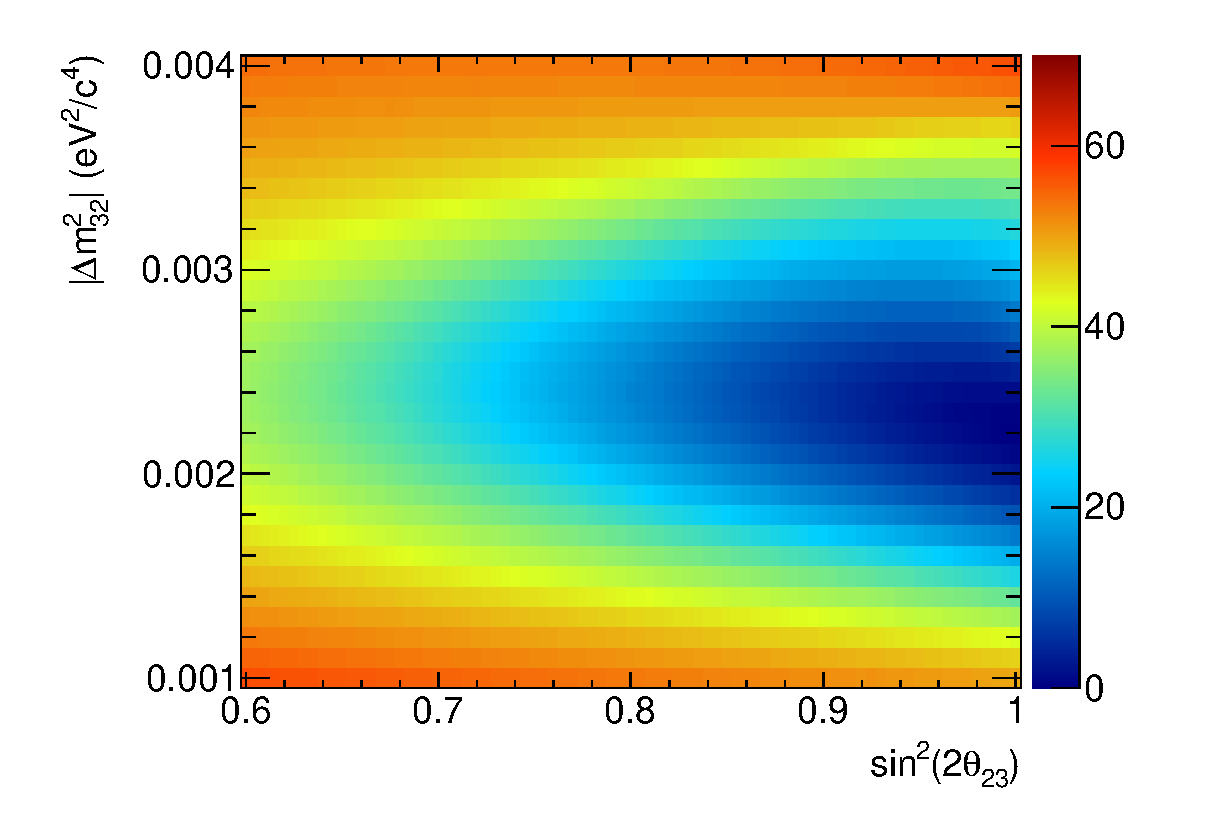
\includegraphics[width=18pc]{./images/fit_toymc/example_fits/dchisq_3}
\caption { 
  $\Delta\chi^2$ surface for the 2+8 fit to fake data set 3
}
\label{fig:fakedata_chisq_3}
\end{minipage}
\vfill
\begin{minipage}[t]{0.48\linewidth}
\center
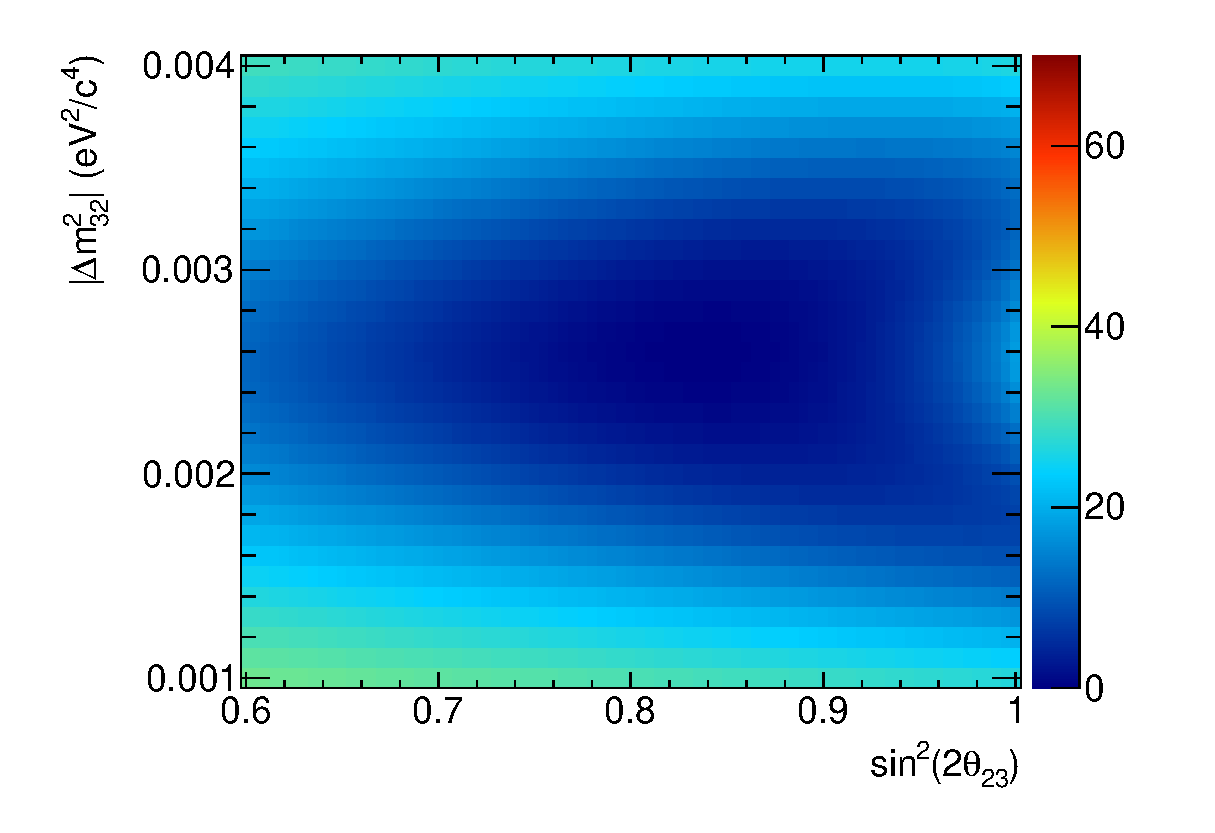
\includegraphics[width=18pc]{./images/fit_toymc/example_fits/dchisq_4}
\caption {
  $\Delta\chi^2$ surface, for the 2+8 fit to fake data set 4
}
\label{fig:fakedata_chisq_4}
\end{minipage}
\hspace{0.06\linewidth}
\begin{minipage}[t]{0.48\linewidth}
\center
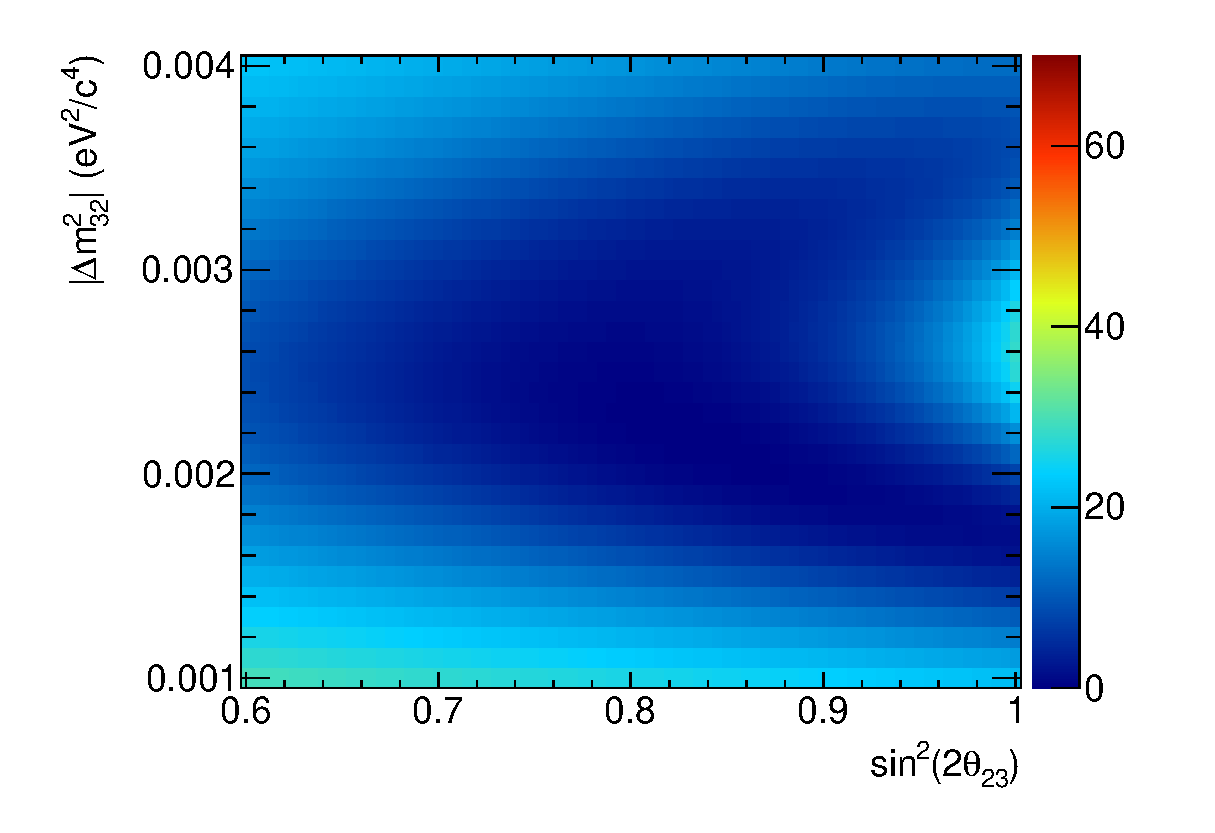
\includegraphics[width=18pc]{./images/fit_toymc/example_fits/dchisq_5}
\caption { 
  $\Delta\chi^2$ surface for the 2+8 fit to fake data set 5
}
\label{fig:fakedata_chisq_5}
\end{minipage}
\end{figure*}


\clearpage
\subsection{Contours}
\label{appendix:example_toy_mc_fits:contours}


%...........................................................
%
% Contours for `2+N' fits
%

\begin{figure*}[htb]
\begin{minipage}[t]{0.48\linewidth}
\center
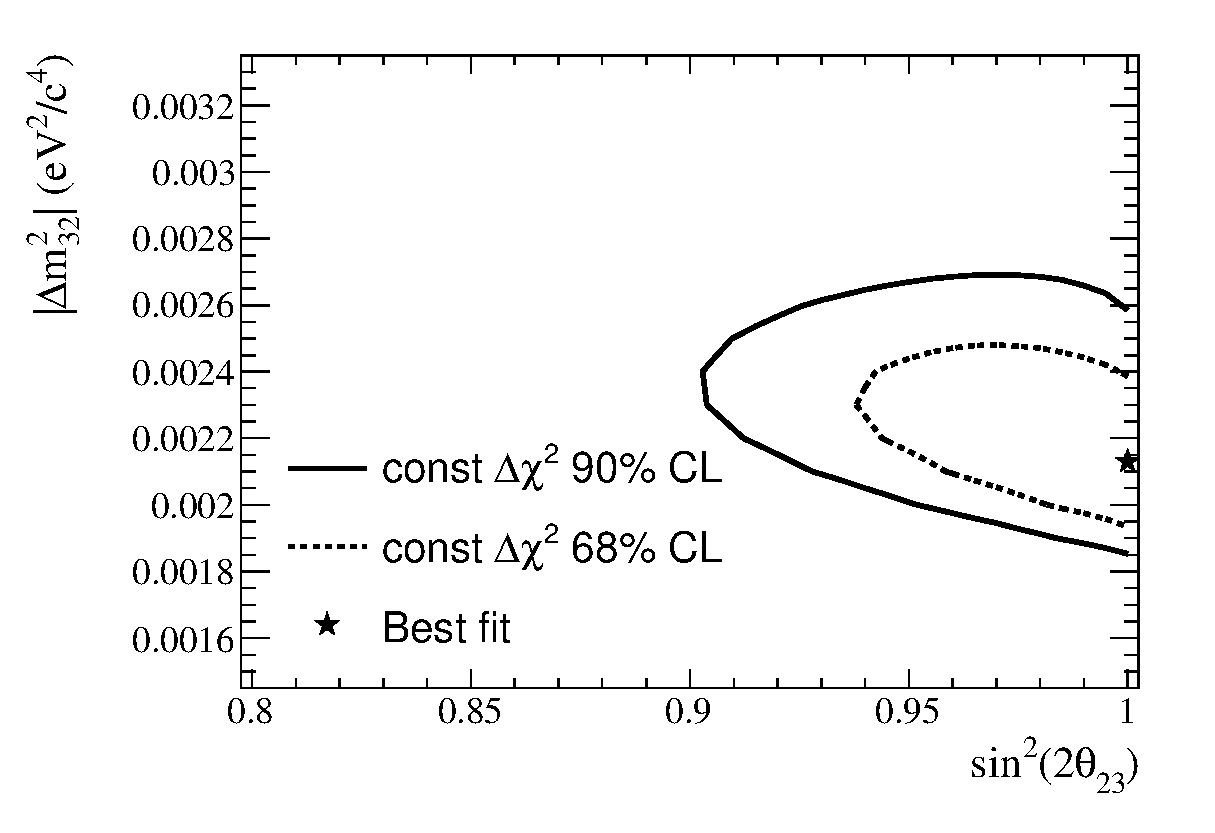
\includegraphics[width=18pc]{./images/fit_toymc/example_fits/2N/contours_0}
\caption {
  68\% and 90\% confidence regions for the 2+N fit to fake data set 0
}
\label{fig:fakedata_contours_2N_0}
\end{minipage}
\hspace{0.06\linewidth}
\begin{minipage}[t]{0.48\linewidth}
\center
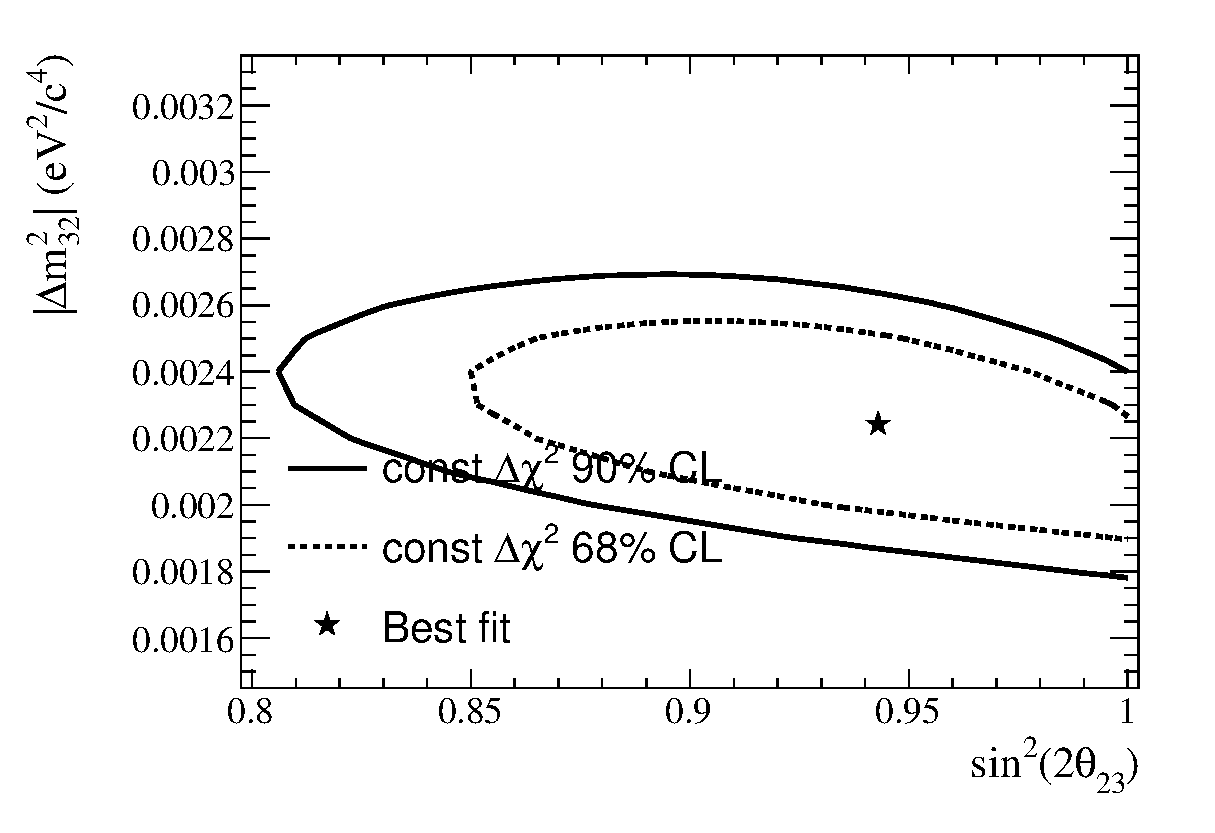
\includegraphics[width=18pc]{./images/fit_toymc/example_fits/2N/contours_1}
\caption { 
  68\% and 90\% confidence regions for the 2+N fit to fake data set 1
}
\label{fig:fakedata_contours_2N_1}
\end{minipage}
\vfill
\begin{minipage}[t]{0.48\linewidth}
\center
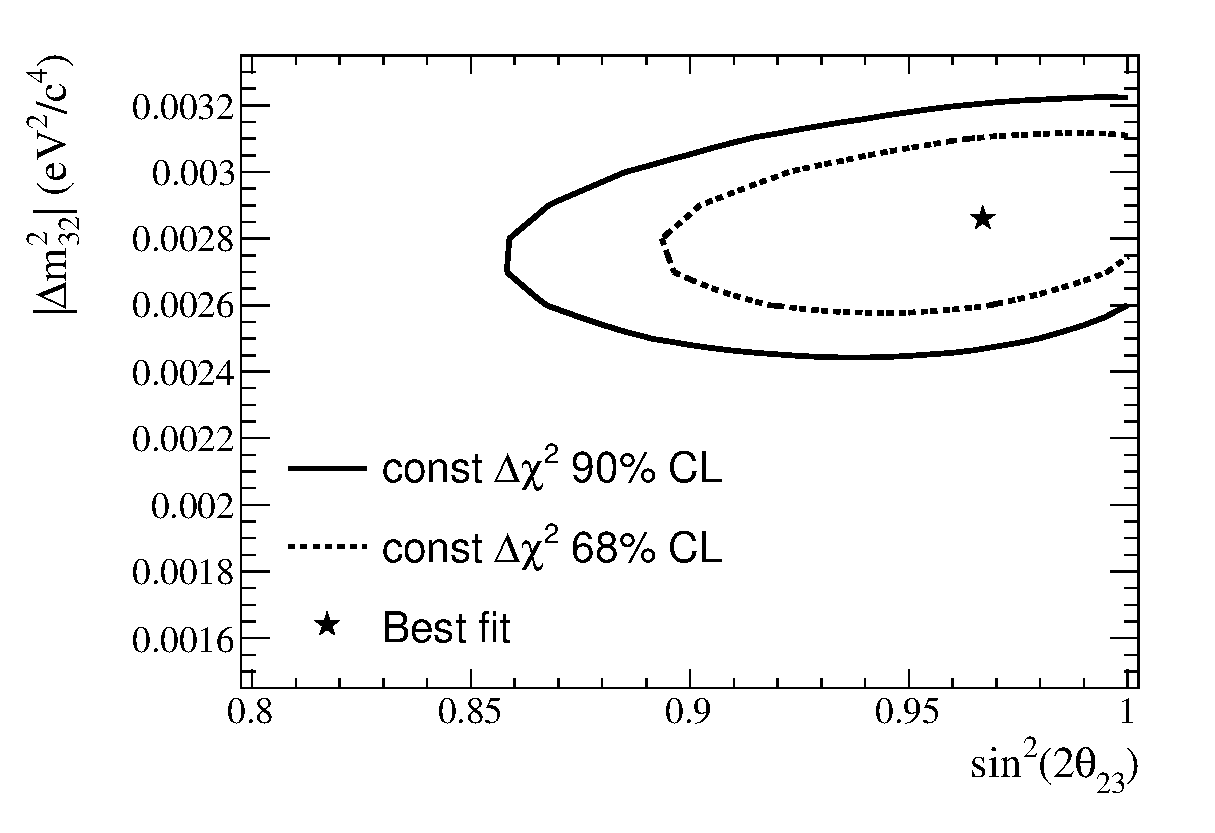
\includegraphics[width=18pc]{./images/fit_toymc/example_fits/2N/contours_2}
\caption {
  68\% and 90\% confidence regions for the 2+N fit to fake data set 2
}
\label{fig:fakedata_contours_2N_2}
\end{minipage}
\hspace{0.06\linewidth}
\begin{minipage}[t]{0.48\linewidth}
\center
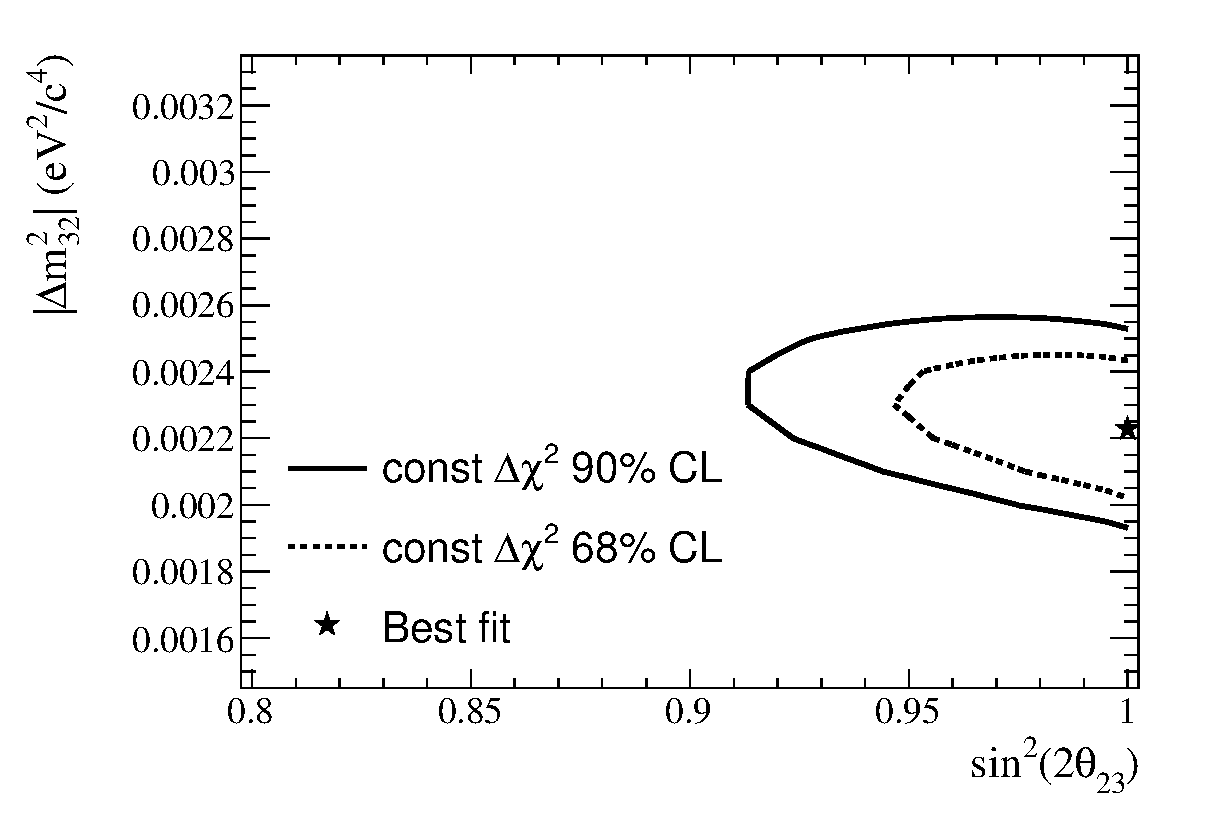
\includegraphics[width=18pc]{./images/fit_toymc/example_fits/2N/contours_3}
\caption { 
  68\% and 90\% confidence regions for the 2+N fit to fake data set 3
}
\label{fig:fakedata_contours_2N_3}
\end{minipage}
\vfill
\begin{minipage}[t]{0.48\linewidth}
\center
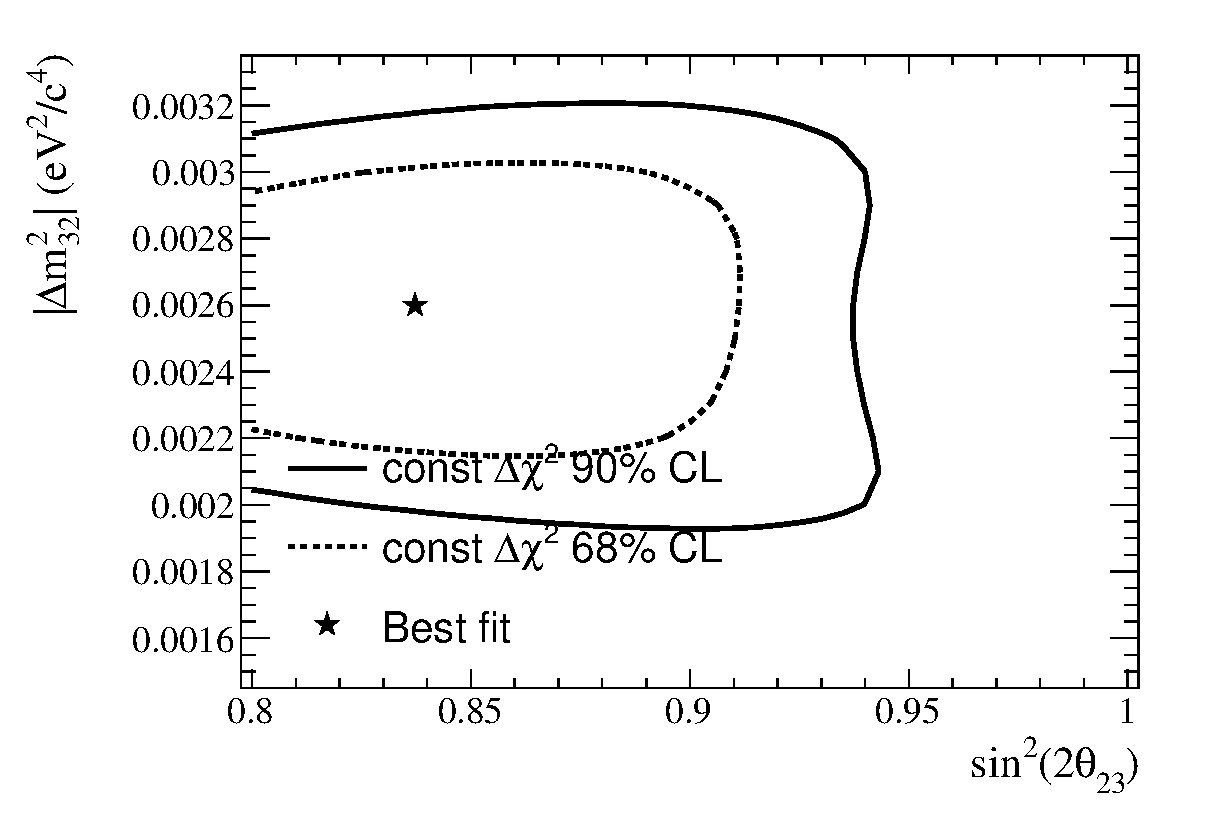
\includegraphics[width=18pc]{./images/fit_toymc/example_fits/2N/contours_4}
\caption {
  68\% and 90\% confidence regions for the 2+N fit to fake data set 4
}
\label{fig:fakedata_contours_2N_4}
\end{minipage}
\hspace{0.06\linewidth}
\begin{minipage}[t]{0.48\linewidth}
\center
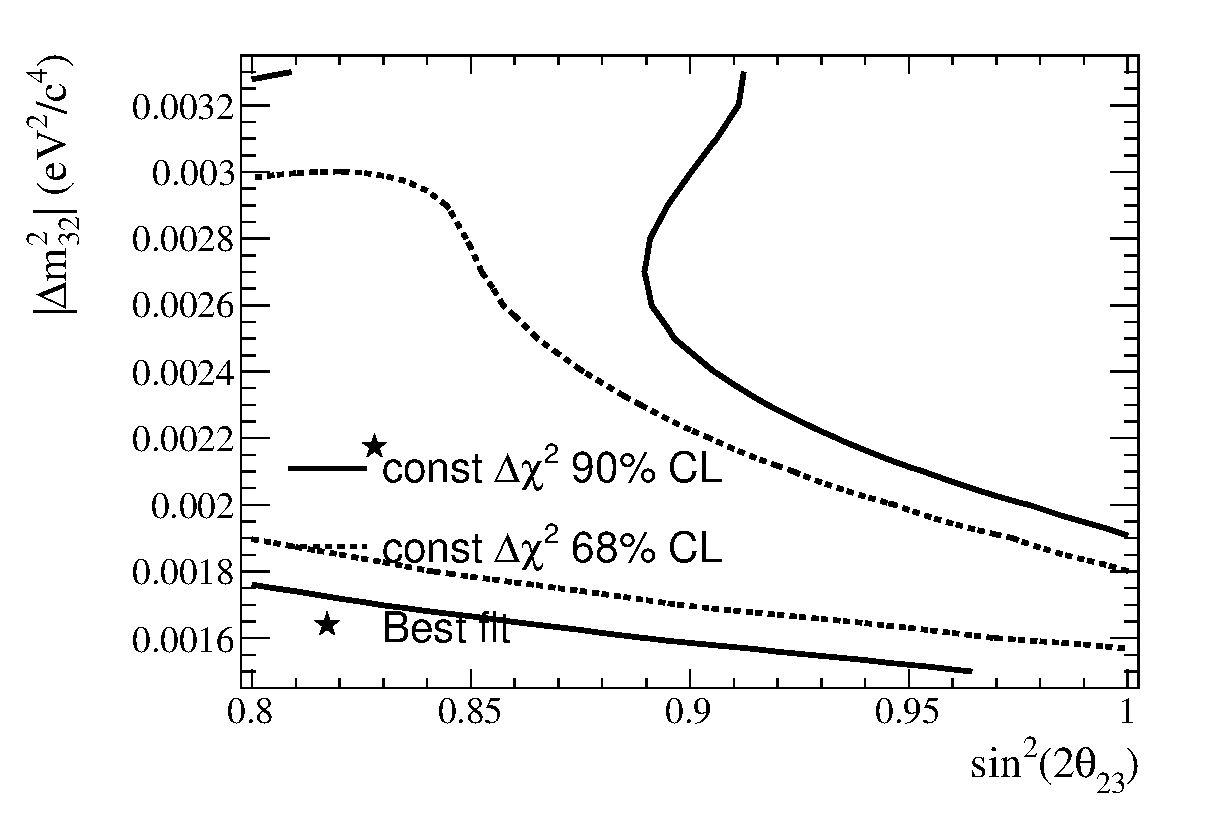
\includegraphics[width=18pc]{./images/fit_toymc/example_fits/2N/contours_5}
\caption { 
  68\% and 90\% confidence regions for the 2+N fit to fake data set 5
}
\label{fig:fakedata_contours_2N_5}
\end{minipage}
\end{figure*}


%...........................................................
%
% Contours for `2+8' fits
%

\begin{figure*}[htb]
\begin{minipage}[t]{0.48\linewidth}
\center
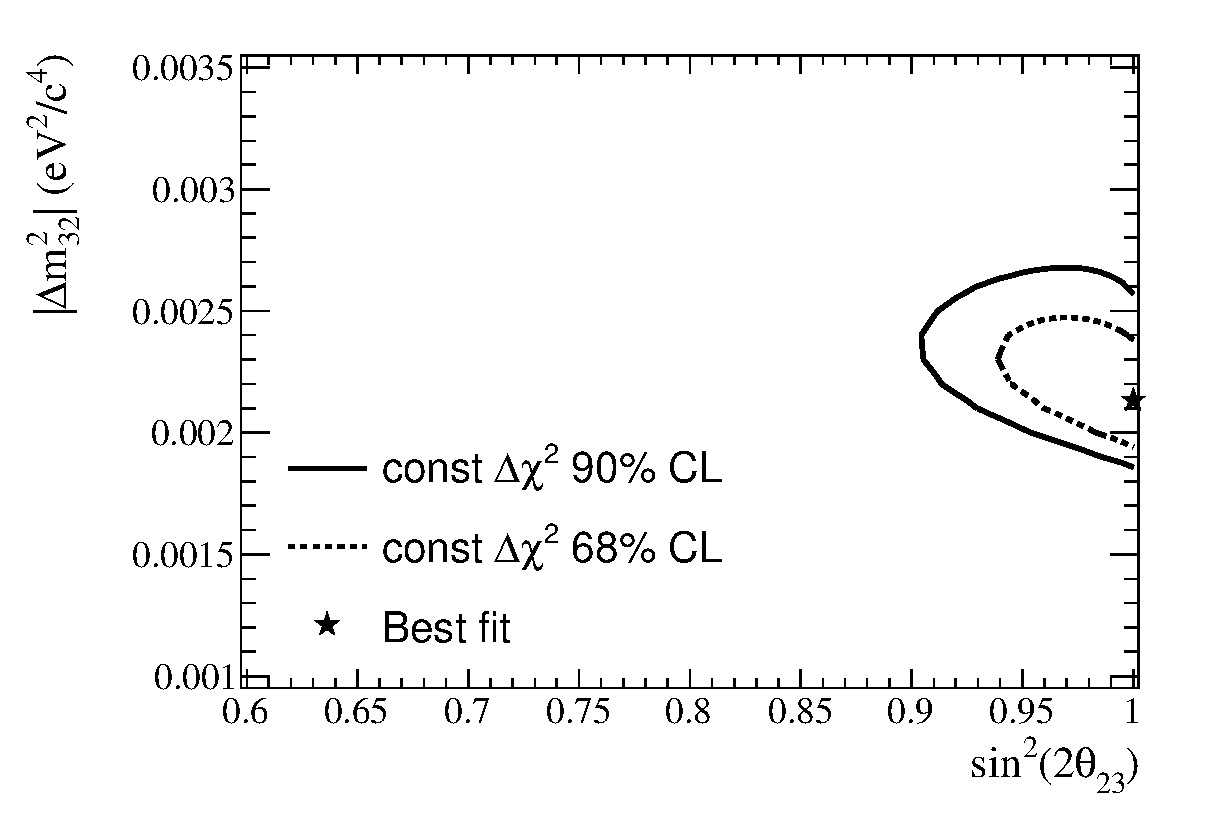
\includegraphics[width=18pc]{./images/fit_toymc/example_fits/contours_0}
\caption {
  68\% and 90\% confidence regions for the 2+8 fit to fake data set 0
}
\label{fig:fakedata_contours_0}
\end{minipage}
\hspace{0.06\linewidth}
\begin{minipage}[t]{0.48\linewidth}
\center
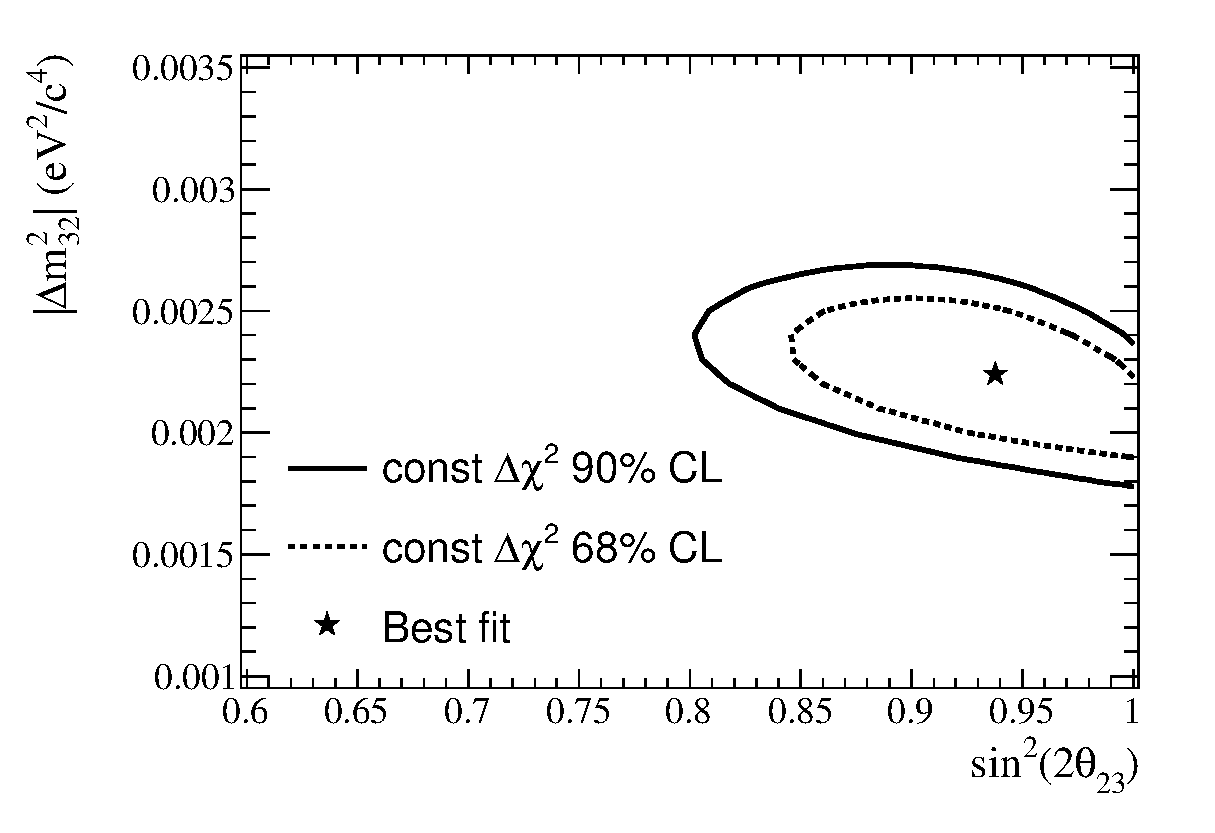
\includegraphics[width=18pc]{./images/fit_toymc/example_fits/contours_1}
\caption { 
  68\% and 90\% confidence regions for the 2+8 fit to fake data set 1
}
\label{fig:fakedata_contours_1}
\end{minipage}
\vfill
\begin{minipage}[t]{0.48\linewidth}
\center
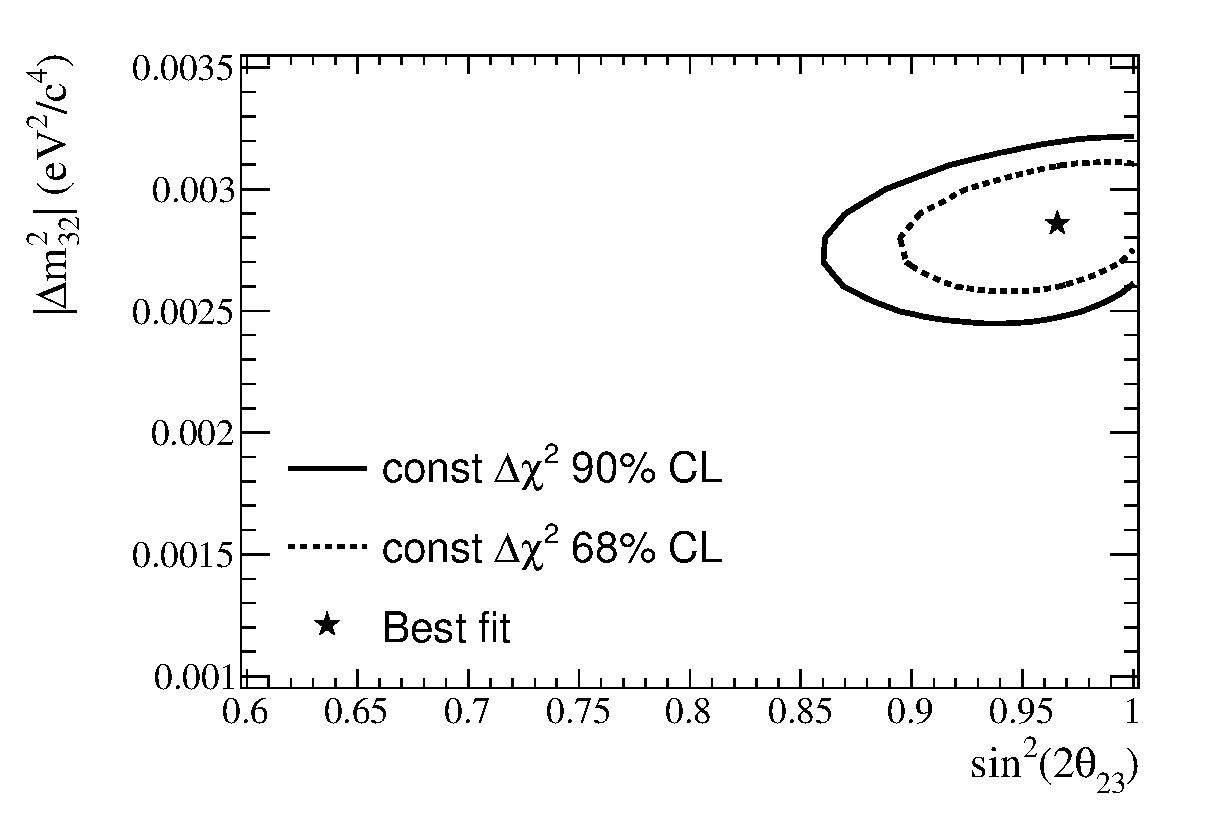
\includegraphics[width=18pc]{./images/fit_toymc/example_fits/contours_2}
\caption {
  68\% and 90\% confidence regions for the 2+8 fit to fake data set 2
}
\label{fig:fakedata_contours_2}
\end{minipage}
\hspace{0.06\linewidth}
\begin{minipage}[t]{0.48\linewidth}
\center
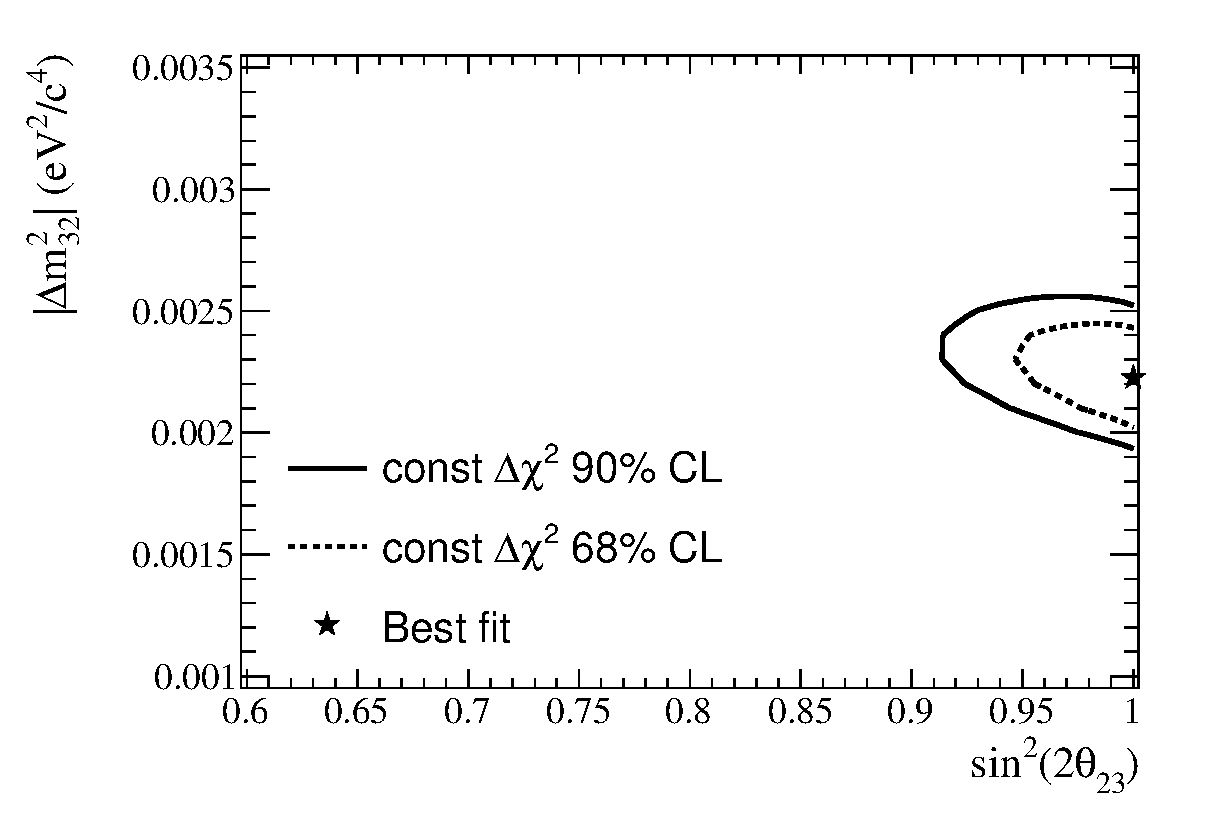
\includegraphics[width=18pc]{./images/fit_toymc/example_fits/contours_3}
\caption { 
  68\% and 90\% confidence regions for the 2+8 fit to fake data set 3
}
\label{fig:fakedata_contours_3}
\end{minipage}
\vfill
\begin{minipage}[t]{0.48\linewidth}
\center
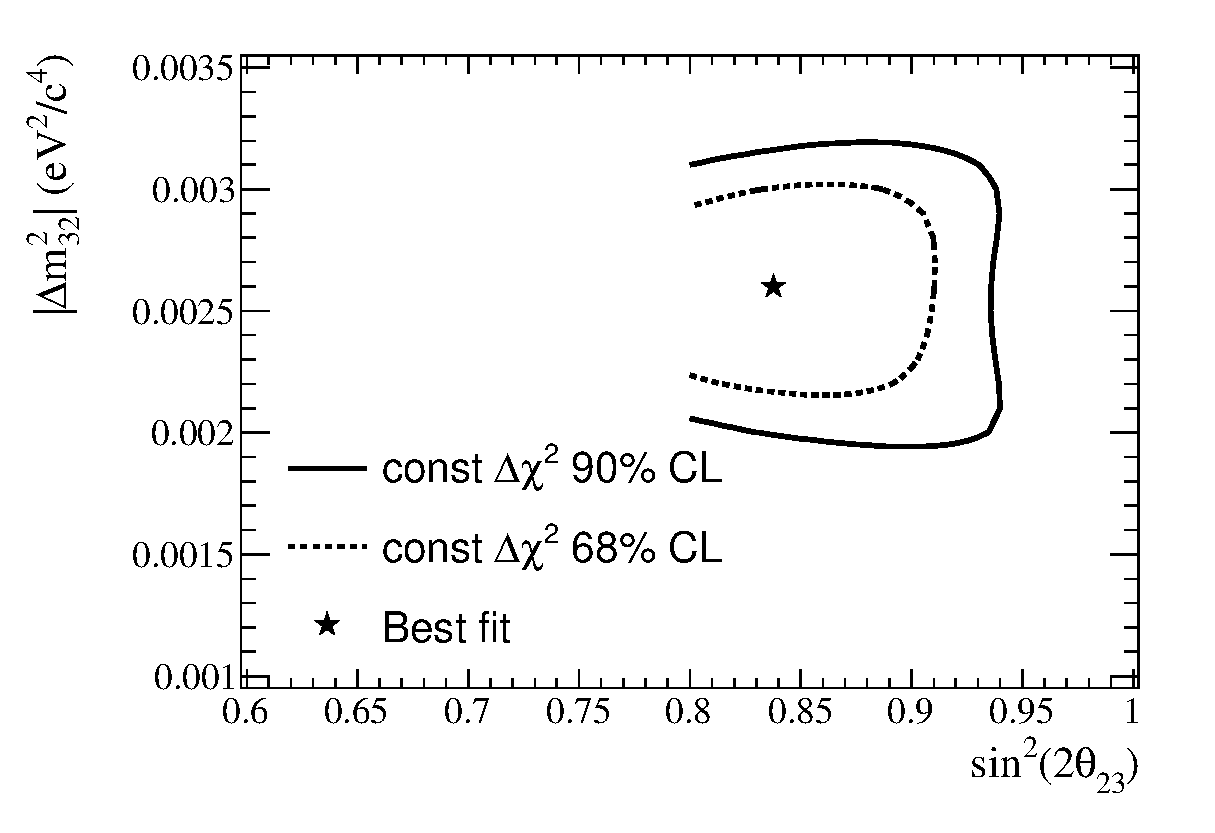
\includegraphics[width=18pc]{./images/fit_toymc/example_fits/contours_4}
\caption {
  68\% and 90\% confidence regions for the 2+8 fit to fake data set 4
}
\label{fig:fakedata_contours_4}
\end{minipage}
\hspace{0.06\linewidth}
\begin{minipage}[t]{0.48\linewidth}
\center
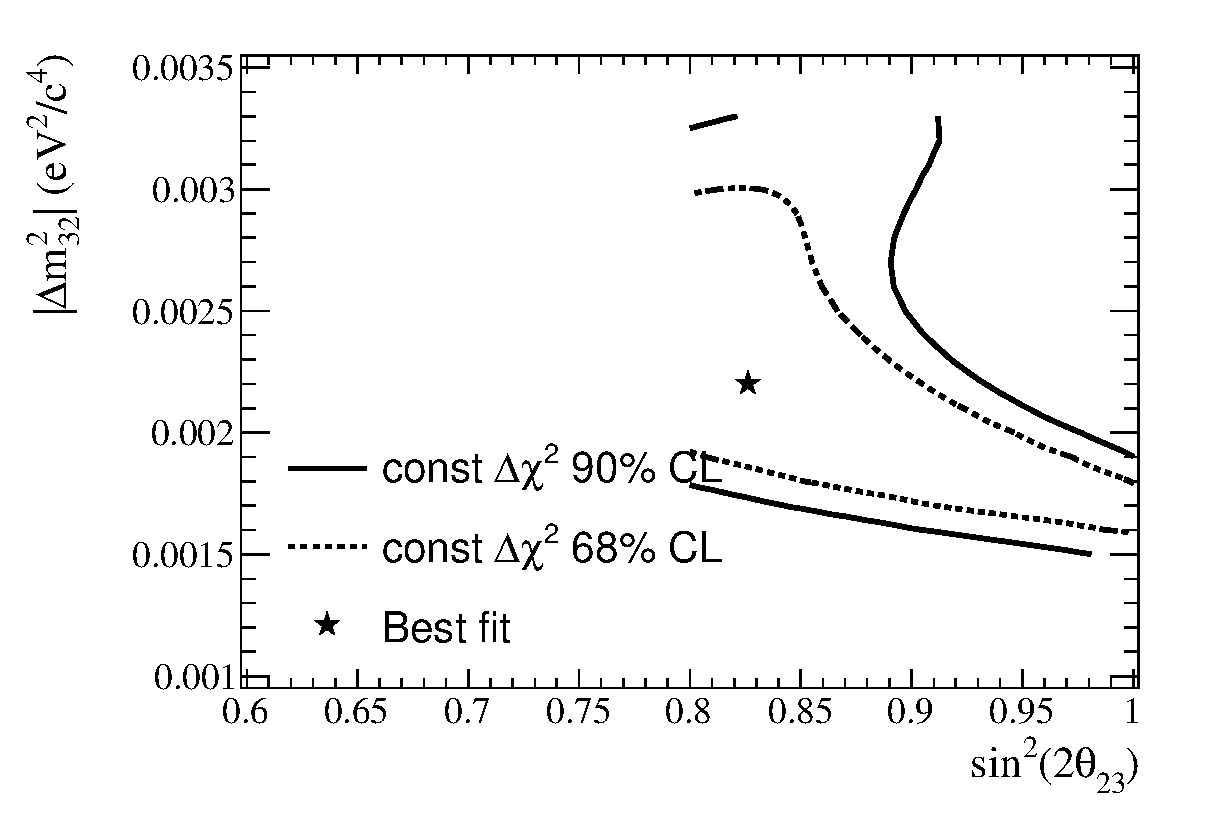
\includegraphics[width=18pc]{./images/fit_toymc/example_fits/contours_5}
\caption { 
  68\% and 90\% confidence regions for the 2+8 fit to fake data set 5
}
\label{fig:fakedata_contours_5}
\end{minipage}
\end{figure*}
